\chapter{Introduction}
\label{cha:Introduction}
Polyketide synthases (PKSs)\nomenclature{PKS}{Polyketide synthases} are large mega-Dalton multi-domain enzyme complexes that synthesize a wide range of natural products of medicinal interest. The structure, dynamics and organization that governs these multi-domain proteins during polyketide biosynthesis is still poorly understood. Developing insight into these systems with the aim of routinely re-engineering them for the biosynthesis of novel compounds, such as anti-cancer drugs and antibiotics, is a long standing goal of many of the PKS research community.

Ever since the inception of the first antimicrobial agent penicillin, observed by Alexander Fleming in the late 1930s, the scientific community has endeavoured to discover new types of antibiotics. From the 1960s to the 1980s the world has seen a boom in the antibiotic industry with the introduction of a diversity of drug variants and classes. However, the introduction of new antibiotics from  the late 1980s till the present date remained stagnant, with very few antibiotics approved by the regulating agencies and also with very few new classes of antibiotics discovered by the scientific community. 

The increasing number of bacterial species acquiring drug resistance and the lack of development in antibiotic discovery has become a threat to humanity. Resistance is now found against almost all classes of antibiotics, even the last line of drugs such as vancomycin \parencite{Alanis2005a, Saga2009}. Drug resistance ranges from single drug resistance to multiple drug resistance \nomenclature{MDR}{Multiple drug resistant}(MDR). Recently bacterial species have been found with extensive drug resistance (XDR) \nomenclature{XDR}{Extensive drug resistant} i.e. resistance to all the available antibiotics except colistin, which is a highly toxic agent and not in regular use. Even worse, the world is facing upcoming issues with pan drug resistant (PDR) \nomenclature{PDR}{Pan drug resistant} organisms, which are resistant to all existing antibiotics including colistin \parencite{Powers2004, Conly2005, Alanis2005a, Saga2009}. 

Although resistant organisms have reached the community and can be found in outpatients the real threat is still to hospitalized patients. Patients in intensive care units, on steroids or with a compromised immune system are readily susceptible to nosocomial infections. Surgical wound infections commonly caused by methicillin-resistant \textit{Staphylococcus aureus} can only be treated with very few antibiotics, e.g. mupirocin. Thus it has become imperative for the scientific community to discover new antibiotics with better efficacy against resistant species. 

Polyketide compounds have shown a variety of medicinal uses, which includes antibiotics. In recent years PKS researchers have shown the capability to re-engineering these pathways in order to produce novel compounds \parencite{Kapur2012, Sugimoto2014}. In the present study I have worked on the biosynthesis pathway of the antibiotic mupirocin. In spite of being potent against skin infections, mupirocin can only be used as a topical drug as it gets systemically metabolised \parencite{Parenti1987}. Furthermore, bacteria such as MRSA, which mupirocin was effective against, are developing resistance. Therefore, remodeling the mupirocin biosynthetic pathway to produce variants is a possible way to increase its usability. Similar methods could also be applied to other PKS systems to enhance features such as the binding affinity, and the metabolic profile of the compounds produced. For example, type I polyketide synthases can introduce \bet-carbon branches into a growing polyketide chain, through tailoring enzyme, allowing introduction of for example a methyl group, halogens or cyclopropane, however it is still not understood what regulates the interaction between the tailoring enzymes and PKSs. Understanding of the underlying mechanism of \bet-branching can be used to instil the \bet-branching capability into non-\bet-branching systems. The dynamic behaviour of the proteins in the pathway, such as acyl carrier proteins (ACPs) that interact with several domains along the pathway, is clearly an important part of these process. 

The present thesis mainly focusses on the \bet-branching mechanism in the mupirocin pathway and on the dynamic behaviour of ACPs. This chapter consists of a general introduction about polyketides, polyketide synthases, challenges and success in polyketide synthase re-engineering, mupirocin biosynthesis and bioinformatics methods available for PKS research. Chapters 3 and 4 presents the results on the computational prediction of the protein-protein interaction involved in the \bet-branching mechanism and the experimental validation respectively. Chapter 5 presents the results on the dynamics of ACPs, and how these might affect recognition process in \bet-branching. Chapter 6 presents the results of two independent projects, first on the ketosynthase specificity towards $ \alpha $-OH substrates in the mupirocin system and the second on molecular dynamics of the loops in ACP-mupA3a + MupH complex assisting the ligand in the MupH active site. Chapter 7 gives the general discussion of the whole thesis. 

	\section{Polyketide}
	\label{sec:Polyketide}
	Polyketides are natural products produced by bacteria, fungi, plants, molluscs, sponges, insects and dinoflagellates; many of these products have medicinal properties,  including antibiotics, antifungal, immunosuppressants, antitumor, antituberculosis and anticholestrol agents (Figure \ref{fig:Polyketides}). As the name suggests polyketides are polymers of simple ketone units synthesized by polyketide synthases (PKSs), which may or may not be further modified by the tailoring enzymes. Due to the diverse nature of modification during the synthesis process, polyketides exist in the form of macrolides, ansamycins, polyenes, polyethers, tetracyclines, acetogenins, and aromatic compounds. Polyketides are produced as secondary metabolites which are non essential for the growth of an organism but may play a crucial role in defence mechanisms, aggression or communication \parencite{Bender1999, Staunton2001, Weissman2005}. 
	
	\setlength\fboxsep{5pt}
	\setlength\fboxrule{1.5pt}
	\begin{figure} [htbp]
	\centering
	\fbox{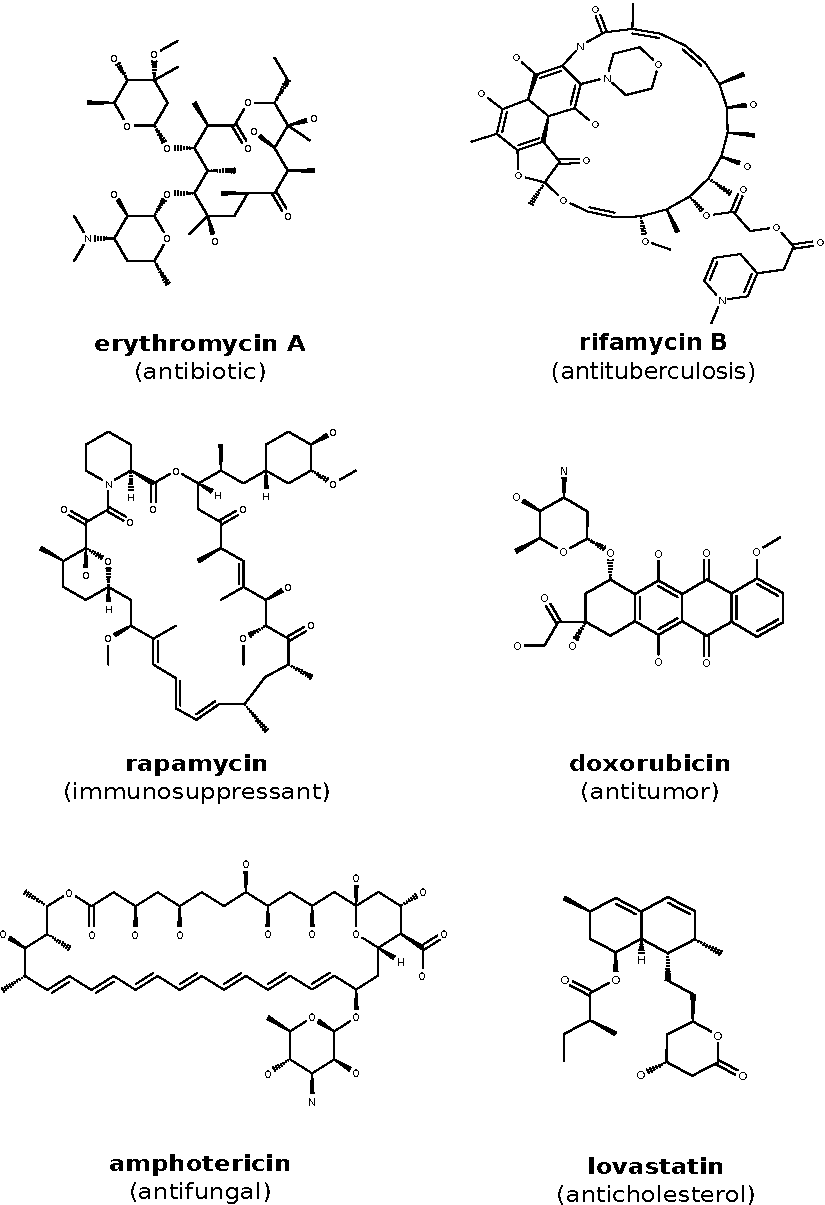
\includegraphics[width=0.9\textwidth, resolution=300, keepaspectratio=true]{graphics/polyketides.pdf}}
	\caption[Example polyketide compounds]{Example polyketide compounds (\url{http://www.drugbank.ca})}
	\label{fig:Polyketides}
	\end{figure}
	
	Polyketide and other natural product based drugs also have a huge market share, which drives pharmaceutical companies to continuously invest in research and manufacturing. Around 10,000 natural products had been identified by the year 1998 and many of these are being used as drugs. Between 1998-2004, 21 natural product based drugs were launched worldwide and around 19 were approved by the FDA between 2005-2010 \Parencite{Mishra2011, Mishra2011A}. Combined sales of erythromycin, FK506 and lovastatin exceeded \textdollar10 billion a year according to a news report in Science magazine published on 1 March, 2001 (\url{http://news.sciencemag.org/2001/03/bugs-making-drugs}).
	
	Polyketide research dates back to 1907 with the John Collie's work at London University on deducing the structure of orcinol \parencite{Collie1907}. However, the main impetus to the field came from Arthur Birch's work on 6-methyl-salicylic acid (6-MSA) produced by \textit{Penicilium patulum} in the 1950s. Arthur Birch explained the mechanism of 6-MSA production based on data from experiments feeding radioactively labelled acetate to the producing strain \parencite{Birch1955}. The labelled product was shown to have the same pattern as was to be expected from Birch's proposed mechanism. These observations of Collie and Birch later on came to be known as the Collie-Birch polyketide hypothesis, which explains that not only these complex natural products were a result of the condensation of simple acetate units, but also that they can be further transformed through enzymatic reactions to produce aromatic or cyclic compounds. 
		
	The detection of these compounds until the 1960s was based on deductive chemistry, where chemists break down the complex molecules into smaller recognizable moieties which were then intuitively assembled on paper \parencite{Powers2004}. Later on the advancement in spectrometric techniques such as mass spectrometry (MS) and nuclear magnetic resonance (NMR) completely transformed the research into easier and more accurate measurements. However, the detailed mechanistic view in the biosynthesis of these compounds and the genes/proteins involved was only possible after 1980s owing to the development of genetic manipulation methods. Genetic methods also enabled the scientific community to realize the potential for \textit{de novo} production of these compounds with altered functional groups. In the present era, with the new concept of synthetic biology, researchers are aiming to design synthetic machineries for the production of novel compounds that can be used for beneficial purposes. 
	
	\section{Polyketide synthases}	
	\label{sec:PKS}
	Polyketides are produced by multi enzyme complexes called polyketide synthases (PKSs). Not surprisingly PKS are equally as complex as polyketide compounds. It was only after the 1980s that researchers were able to characterize the genes and proteins involved in the PKS. The very first genes for a PKS were characterized by David Hopwood's group in 1984, for actinorhodin, an aromatic polyketide compound \parencite{Malpartida}. Later on Peter Leadlay and Leonard Katz independently identified the gene cluster responsible for the antibiotic erythromycin produced by \textit{Saccharopolyspora erythraea} \parencite{Cortes1990, Tuan1990}.
	
		\subsection{FAS and PKS analogous reaction mechanism}
		\label{sec:FAS}
		PKS share sequence and mechanistic similarity with the very well studied fatty acid synthases (FAS) \nomenclature{FAS}{Fatty acid synthase}. FAS synthesizes a relatively small group of saturated compounds as compared to the myriad of polyketides. Fatty acids are produced by a monotonous process of decarboxylative condensation of two ketone units followed by a series of reductive steps till a fully saturated molecule is achieved. The acyl transferase (AT) \nomenclature{AT}{acyltransferase} domain loads the starter (acetyl) and the extender units (malonyl) to the acyl carrier protein (ACP), \nomenclature{ACP}{Acyl carrier protein} which covalently tethers the ligand via a thioester bond to the long phosphopantetheine arm. The ACP transfers the starter or the extender units to the ketosynthase (KS) \nomenclature{KS}{Ketosynthase} for the decarboxylative condensation and also carries the newly synthesized product to be passed on to the other domains for further processing. Acting successively, keto reductase (KR) \nomenclature{KR}{Ketoreductase} reduces the \bet-keto group to a hydroxyl which is further reduced by a dehydratase (DH) \nomenclature{DH}{Dehydratase} to produce an alkene, this double bond is then reduced to a fully saturated chain by an enoyl reductrase (ER). \nomenclature{ER}{Enoyl reductase} The process of decarboxylative condensation and successive reductions continue till the fatty acid chain reaches to a required length, where upon it is then released by the thioesterase (TE) \nomenclature{TE}{Thioesterase} domain.
				
		Both PKS and FAS enzyme systems can be classified into type I, II, with an additional type III for PKS (more detail on PKS types in Section \ref{sec:PKStypes}). Type I FASs as found in mammals and fungi, are large multi domain complexes where the catalytic domains are covalently linked together in a long polypeptide chain. A single set of seven catalytic domains, as mentioned above, are utilized to produce a single molecule of fatty acid of the required length. Whereas, the type II FASs are free standing discrete mono functional catalytic units, used iteratively. Type II FASs are commonly found in bacteria, chloroplasts and mitochondria.
					
		In comparison to FAS machinery, PKS machinery is more complex and dynamic. PKSs vary the reductive steps on the \bet-keto acyl moiety after the condensation has happened, thus producing products with combinations of non modified \bet-keto groups, hydroxyl and enoyl groups. Several type I modular PKS were also found with modules lacking any condensation activity, for example the module 5 in the mmpA subunit of the mupirocin system. PKSs also have a choice of various starter and extender units \parencite{Khosla1999, Staunton2001}, in contrast to FASs which always start with acetyl and malonyl as the starter and extender unit respectively. Among many possible examples, of polyketide antibiotic pathways which utilize non conventional starter and extender units, as compared to the FAS, two examples are aureothin synthesis, which incorporates p-nitrobenzoate as the starter unit, and the erythromycin system which utilizes (2S)-methylmalonyl-CoA as the extender units.  PKS products are usually modified by various types of tailoring enzymes working \textit{in trans} for purposes such as cyclization, beta branching, epoxidation, pyran ring formation etc. Figure \ref{fig:FASandPKS} shows the generic reaction mechanism carried out by the FAS and PKS.
		
		\setlength\fboxsep{5pt}
		\setlength\fboxrule{1.5pt}
		\begin{sidewaysfigure} [htbp]
		\centering
		\fbox{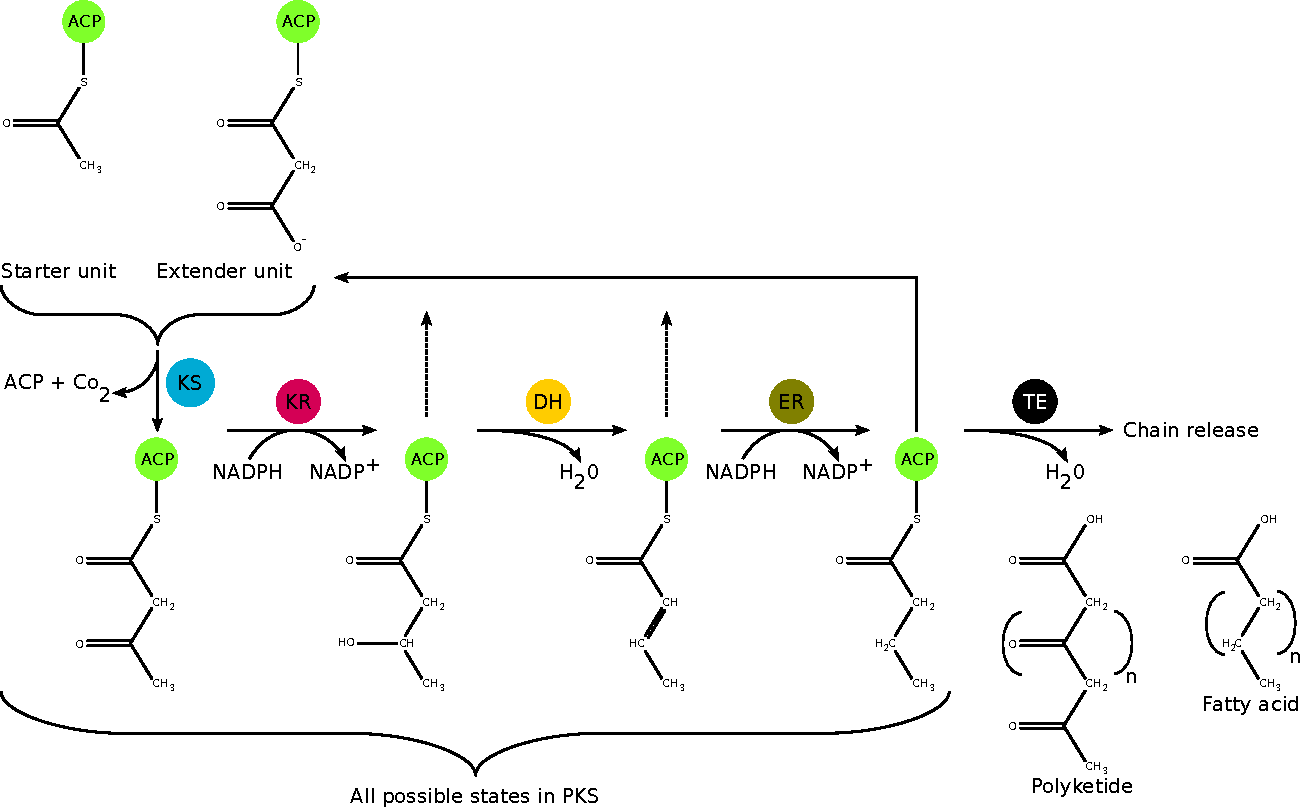
\includegraphics[width=0.9\textwidth, resolution=600, keepaspectratio=true]{graphics/FASandPKS.pdf}}
		\caption[Generic reaction mechanism for FAS and PKS]{Generic reaction mechanism for FAS and PKS. ACP: Acyl carrier protein; KS: Ketosynthase; KR: Ketoreductase; DH: Dehydrates; ER: Enoyl reductrase; TE: Tioesterase. In FAS the \bet-keto moiety in the elongated product is completely reduced to an acyl moiety as compared to the PKS in which it may or may not be partially or completely reduced thus producing keto, hyroxy and enoyl products. }
		\label{fig:FASandPKS}
		\end{sidewaysfigure}
		
		\subsection{FAS and PKS models}
		\label{sec:FASmodels}
		Over the years many research groups have proposed the likely domain organization and structural models for the FAS and PKS systems. The very first model proposed and widely accepted was the head to tail model in the 1970s which was later on overtaken by a newer head to head model for the FAS system and subsequently for the PKS as well. These simple models based on the domain organisation of the gene cluster and a few crosslinking experiments, helped researchers to understand FAS and PKS assembly until augmented by more accurate atomic resolution structures for full length FAS that were determined through X-ray crystallography. Although, researchers managed to successfully determine the structures for the FAS from various organisms we still lack a complete structure of a PKS. Some recent efforts have indeed produced structures of individual or binary domains from different PKS systems but a complete picture of an entire subunit or a module with all the catalytic domains is still missing.
			
			\subsubsection{Head to tail/head models for FAS}
			\label{sec:heatotail}
			Evidence in the 1970s and 1980s seemed to support the existence of a head to tail model for FAS structure and function (Figure \ref{fig:headandtail} A), but this was eventually superseded by a head to head model (Figure \ref{fig:headandtail} B)  In the 1970s many researchers observed that FAS mono functional units fail to catalyse chain elongation. FASs can be reversibly dissociated into functional units on exposure to low ionic strength buffers at cold temperature; the function restores in high ionic media at room temperature \parencite{Kumar1970,Smith1971}. The loss of elongation implied that for condensation to happen the active cite cysteine of the ketosynthase needs to be in close proximity of the phosphopantetheine arm of the ACP. Later on it was discovered that the active site cysteine of one subunit can be cross linked to the phosphopantetheine of the ACP on the other subunit by 1,3-dibromopropanone. This cross linking experiment was interpreted as meaning that the condensation required the interaction of KS and ACP from the opposite subunits \parencite{Stoops1983}. Another experiment on the FAS dimer with blocked thioesterase, showed two hanging fatty acids \parencite{Singh1984}. Additionally sequence analysis revealed that the ACP is located far away from the KS on the FAS cluster. Thus the above observations seemed to support the fully extended head to tail model where there were two reaction sites which were coordinated by the ACPs from the opposite subunit. 
		 	
		 	\setlength\fboxsep{5pt}
		 	\setlength\fboxrule{1.5pt}
		 	\begin{figure} [htbp]
		 	\centering
		 	\fbox{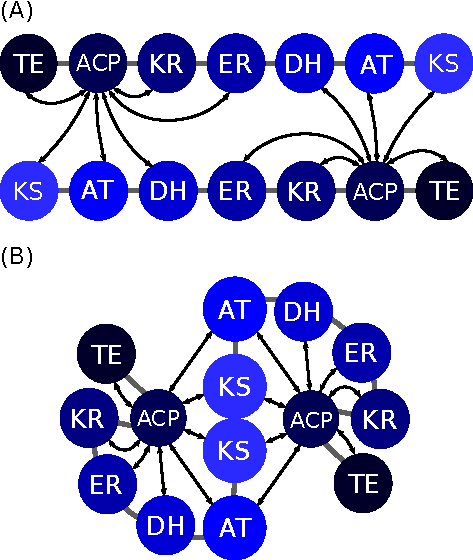
\includegraphics[width=0.8\textwidth, resolution=600, keepaspectratio=true]{graphics/headandtail1.pdf}}
		 	\caption[Head to tail/head models for FAS]{Head to tail/head models for FAS. (A) The fully extended head to tail model (B) The coiled head to head model. Figure adapted from \textcite{Smith2007}. }
		 	\label{fig:headandtail}
		 	\end{figure}
		 				
					
			Thus, the head to tail model gained a wide acceptance till it was challenged on the basis of the mutant complementation experiments. The complementation experiments showed that in the animal FAS the KS and ACPs can function together on either subunit \parencite{Witkowski1996}. Joshi and co-workers from the Smith group created several mutant knockouts in which different domains were inactivated. These mutant subunits were made to re-associate to create a mixed population of hetero and homo dimers. There findings revealed that homodimers formed by the KS, ACP, DH or TE mutant knockouts (at least one point mutation) and the hetero dimers formed by the ACP and TE mutant, ACP and DH mutant and DH and TE mutants were unable to carry out synthesis. However, heterodimers formed by KS and either DH, ACP, or TE mutants were able to carry out the synthesis at a reduced rate. These observations showed that the ACP and DH which are located far on the same subunit were able to interact which suggest that it was not necessary for the FAS to be in fully extended head to tail conformation. On the other hand a coiled state would explain the ability of the far placed ACP and DH to interact \parencite{Joshi1997,Joshi1998}.
		 	
		 	These observations lead to  questioning the interpretation of previously conducted crosslinking experiments, which had showed that 1,3-dibromopropanone can be used to cross link the active cite cysteine of ketosynthase to the phosphopantetheine arm of the ACP. The re-examination of the original cross linking experiment data revealed three bands, which would correspond to the double cross linked inter subunit species, single cross linked inter subunit species and single cross linked intra subunit species. If the interaction of the head to tail model, as in Figure \ref{fig:headandtail} (A), held true then there would have been only two bands for the single and double inter cross linked species. The presence of the third band indicates the possibility of the intra subunit KS - ACP interaction.
		 	
		 	To put the last nail in the coffin of the head to tail model, Joshi and co workers created an engineered mammalian FAS with only one functional subunit, all the domains from the other subunit were inactivated. This engineered FAS was able to catalyse all the biosynthetic steps in the fatty acid synthesis \parencite{Joshi2003}. These observations were enough to refute the requirement of the fully extended state of the head to tail model but would rather support the requirement of a scaffold which allows the domains on the two subunits to be accessible to their companion domain (Figure \ref{fig:headandtail} (B)).
		 	
 			This scaffold would support the newer head to head model in which the KS forms a dimer at the centre and the flanking domains coil around it, instead of KS being at the polar ends as in the head to tail model as  shown in Figure \ref{fig:headandtail} (A). This model also agrees with the KS in the FAS type II in which the KSs are known to exist as homo dimers and the active site is formed by the contribution of both the subunits \parencite{Moche1999, Olsen2001, Price2003}. Experiments carried out by Witkowski and co-worker showed that a truncated N terminal FAS (i.e. with incomplete KS) fails to dimerise. They also showed that the two KS subunits can be  cross linked via an engineered cysteine at the N terminal of the KS at a close proximity of 6 \AA{}. This crosslinking failed if one of the subunits lacks an engineered cysteine. They concluded their observation by performing mass spectrometry on the digested  cross linked product \parencite{Witkowski2004}.
 			
 			\subsubsection{Models for modular PKS}
 			\label{sec:CamPKS}
 			In the 1990s groups from the USA and UK lead by Khosla and Cane, and Staunton and Leadlay respectively, proposed the likely models for modular PKSs. The independent studies carried out by both the groups on the DEBS system using different methods agreed on the presence of two catalytic chambers for the condensation reaction in the modular PKSs. The studies also confirmed the dimeric nature of the PKSs similar to FASs. However, the proposed models by the two groups were strikingly different, details of which are discussed below. 
 			
 			The UK group in a series of experiments carried out limited proteolysis of the DEBS subunits using four proteases. The different sized fragments produced due to proteolysis were identified using N-terminal sequencing. They also determined the oligomeric state of the fragments using gel filtration and analytic ultracentrifugation. All the large fragments carrying the complete module were found to be homodimeric. The loading domain and the AT-ACP domains of the module 1 were found to be monomeric along with all the KR and ER domains in module 1,3,5 and 6 and module 4 respectively. On the basis of the cross linking experiment carried on the FAS (as mentioned in the previous section), the UK group used 1,3-dibromopropanone to cross link the 4'-phosphopantetheine moiety to the cysteine in the KS active site. The cross linking experiment confirmed an interaction between the KS and ACP from the opposite subunits \parencite{Aparicio1994, Staunton1996}.  
 			
 			These observations laid the basis for two models for the modular PKS, which were proposed to be parallel dimers. In the first model they proposed parallel dimers formed by the interaction of the KS and ACP at the interface and the other reductive domains protruding outwards from the axis, keeping all the domains at the reachable distance of the 4'-phosphopantetheine arm. In the second model (which alter came to be known as \textbf{Cambridge model}) the parallel dimers form a helical core utilizing KS, AT and ACP and the reductive domains again protrude away from the axis. Both the models showed the possibility of stacking multiple subunit on top of each other without affecting the functioning of the biosynthesis pathway. However, on the basis of the ultra-centrifugation results, that the protein dimer does not dissociate even at very low concentrations, the helical model was predicted and favoured to be more stable structure. These observations also proposed the inherent ability of the PKS to accommodate additional PKS which can be stacked with the rest of multi enzymes. Since the reductive domains protrude outside the dimeric core there is also a possibility of adding diversity to the reductive steps \parencite{Aparicio1994,Staunton1996}, as represented in Figure 3 A and B of \textcite{Staunton1996}.
 			
 			At the same time Khosla and Cane worked on finding the evidence for the domains participating in polyketide biosynthesis by generating several active site mutant PKSs. The experiments were performed \textit{in vitro} using DEBS 1 + TE, which consist of two modules along with an engineered TE domain. DEBS 1 + TE produces a cyclic triketide by utilizing propionyl-CoA and (2RS)-methylmalonly Co-A as starter and extender units respectively, and NADPH as the hydride donor. These experiments were carried out with the assumption that the modular PKS forms head to tail homodimers similar to the then prevalent idea for  mammalian FASs. In one study they produced three different active site DEBS 1 + TE mutants in which either the KS from module 1 or 2 or the ACP from module 2 was inactivated, refered to as KS1$ ^{0} $, KS2$ ^{0} $ and ACP2$ ^{0} $. These three parental mutant homodimers were utilized to produce three mutant heterodimers in which heterodimer a) consist of KS1$^{0}$ and KS2$^{0}$ , b) consist of KS2$^{0}$ and ACP2$^{0}$ and c) consist of KS1$^{0}$ and ACP2$^{0}$. The first two heterodimers were found to be active and were able to produce the triketide moiety however, the heterodimer c was unable to produce the triketide product. These observations gave substantial evidence that polyketide biosynthesis is based on the participation of two sets of active sites from opposite subunits and the cognate pair of KS and ACP can only be involved in the chain transfer \parencite{Kao1996}. These results were in contrast to FAS biosynthesis which allows chain elongation through either the KS-ACP pair from the opposite subunit or from the same. 
 			
 			In another study, following a similar mutant complementation strategy, Khosla and coworkers created an AT null mutant. This AT mutation was carried out in the module 2 and was paired with either the KS1$^{0}$ or KS2$^{0}$ mutants, thus generating two pairs of heterodimers. The aim of the experiment was to test whether the AT2 domain would be able to load the methylmalonyl extender unit to ACP2 from the same or the opposite subunit. If the loading of the extender unit is similar to the KS-ACP interaction from the opposite subunit then only the heterodimer carrying KS1$^{0}$ and AT2$^{0}$ should be active and not the heterodimer carrying KS2$^{0}$ and AT2$^{0}$. The complementation experiment showed that both the heterodimers were active and the AT domain were able to load the extender unit both inter and intra subunit. Kinetic studies showed no difference in the rate of extender unit loading  between the intra or inter subunit transfer \parencite{Gokhale1998}. 
 			
 			 	
		\subsection{Types of polyketide synthases}
		\label{sec:PKStypes}
		As mentioned in the previous sections, PKSs can be classified into three types, I, II and III where type I and II PKS are similar to FAS type I and II. Apart from the three canonical PKS types various PKS systems exist as hybrid with one or more other types. Hybrids also exists between one of the PKS types and a closely related non PKS system called non ribosomal peptide synthases (NRPS). The following sections describe the different PKS types in detail with relevant examples. 
			
			\subsubsection{Type I PKS}
			\label{sec:typeIPKS}
			Type I PKS are large single polypeptide multi domain protein complexes which can be further sub classified into modular and iterative types. As the name suggests, modular type I PKSs are composed of multiple modules where each module consists of all the necessary domains required for a single round of polyketide chain elongation and associated \bet-carbon processing. Whereas type I  iterative PKSs utilize a single set of covalently bound catalytic domains iteratively until the required length of the polyketide product with correct \bet-carbon processing is reached \parencite{Hertweck2009}. Type I modular PKSs are usually found in bacteria, for example the DEBS system in \textit{Saccharopolyspora erythraea} (Figure \ref{fig:DEBS}), whereas type I iterative PKSs are found in fungi for example the lovastatin system in \textit{Aspergillus terreus} (Figure \ref{fig:lov}). Type I modular PKSs can also be further classified as \textit{cis} and \textit{trans}-AT systems. \textit{Cis}-AT systems (e.g. DEBS) consist of a covalently fused AT domain within each module, which is responsible for loading the extender unit specific for the cognate module. Where as in \textit{trans}-AT systems (e.g. mupirocin) the AT domain is not covalently fused within each module but it exists as a separate discrete domain. \textit{Trans}-ATs are responsible for loading the starter unit at the beginning of the pathway as well as the extender units at each module throughout the pathway. 
			
			In type I modular PKSs since each module is responsible for a single step of chain extension and subsequent \bet-carbon processing, it is possible to deduce the product being produced just by studying the sequence in which the modules are arranged in the biosynthetic cluster. This collinearity rule has enabled the development of various computational methods to predict the probable metabolite being produced directly from the DNA or protein sequence. Section \ref{sec:BioinfoPKS} gives a more detailed account of the computational methods developed till now to predict the polyketide as well as other secondary metabolites from their biosynthetic gene/protein cluster. Although this collinearity rule in type I modular PKSs is effective in predicting metabolite production straight from the sequence, it does not hold true in \textit{trans} AT systems and in systems where a certain module is used iteratively or skipped altogether. 
			
			\setlength\fboxsep{5pt}
			\setlength\fboxrule{1.5pt}
			\begin{sidewaysfigure} [htbp]
			\centering
			\fbox{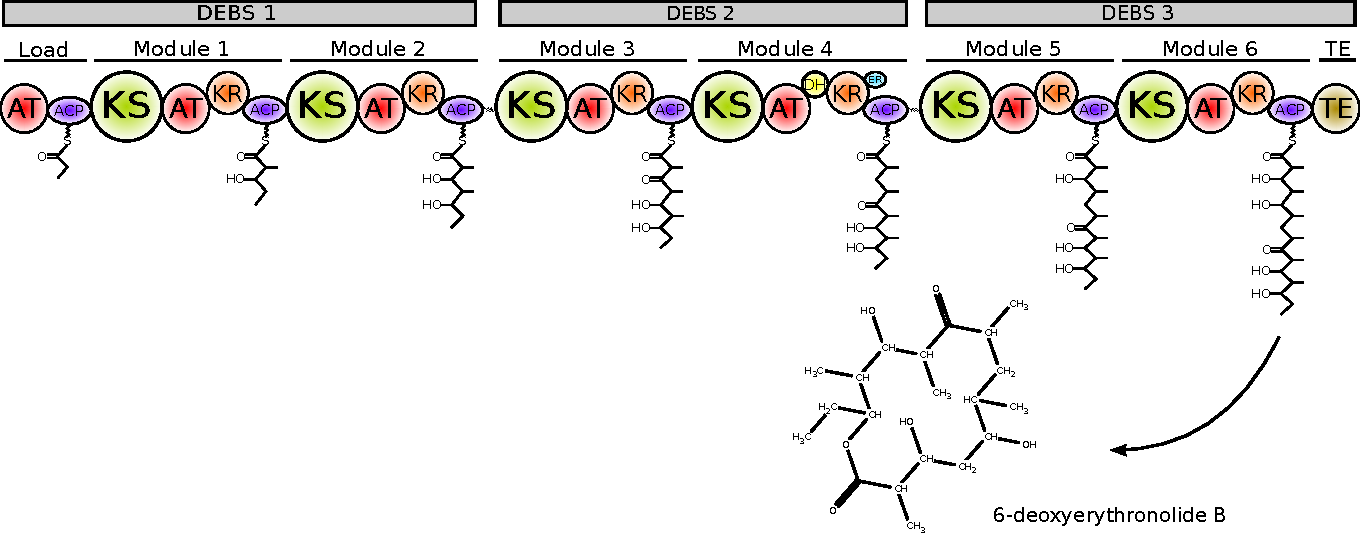
\includegraphics[width=\textwidth, resolution=600, keepaspectratio=true]{graphics/debs.pdf}}
			\caption[Type I polyketide synthases (modular and cis AT) from 6-deoxyerythronolide B synthase
			(DEBS) system.]{Type I polyketide synthases (modular and cis AT) from 6-deoxyerythronolide B synthase
			(DEBS) system.  The DEBS system consist of 28 domains spread across 3 polypeptides (DEBS 1, 2 and 3) of ~350 kDa each, with each polypeptide containing two modules. Abbreviatiosn: KS, ketosynthase; AT, acyltransferase; ACP, acyl carrier protein; KR, ketoreductase; KR 0, inactive ketoreductase; DH,
			dehydratase; ER, enoylreductase. Figure adapted from \parencite{Khosla2007}
			}
			\label{fig:DEBS}
			\end{sidewaysfigure}
			
			For many years DEBS served as the model system for studying type I modular PKS. DEBS is responsible for the production of 6-deoxyerythronolide B which acts as a precursor in the production of the  antibiotic erythromycin. The DEBS system consists of 28 domains spread across 3 polypeptides (DEBS 1, 2 and 3) of ~350 kDa each, with each polypeptide containing two modules (Figure \ref{fig:DEBS}). DEBS 1 contains an extra module which consists of an AT and ACP domain prior to the condensing module 1. This extra module is responsible for priming the KS in module 1 with a propionate unit. DEBS 3 contains a TE domain after module 6, for polyketide release. Each module in the DEBS system is responsible for a single round of Claisen condensation utilizing methyl malonate as the extender unit. Every module in the DEBS system also performs \bet-keto reduction of the condensed product and only module 4 further reduces the \bet-carbon with a dehydratase and an enoyl reductase (Figure \ref{fig:DEBS}) \parencite{Khosla2007}. Due to the modular nature of the DEBS system and ease of cloning the DEBS genes into an appropriate host like \textit{S. coelicolor} and \textit{E. coli}, many research groups exploited the DEBS machinery to understand and elaborate the re-engineering capability of modular type I PKSs. Section \ref{sec: reengineer} explains an example of successes and challenges in re-engineering PKSs.  
			
			\setlength\fboxsep{5pt}
			\setlength\fboxrule{1.5pt}
			\begin{figure} [htbp]
			\centering
			\fbox{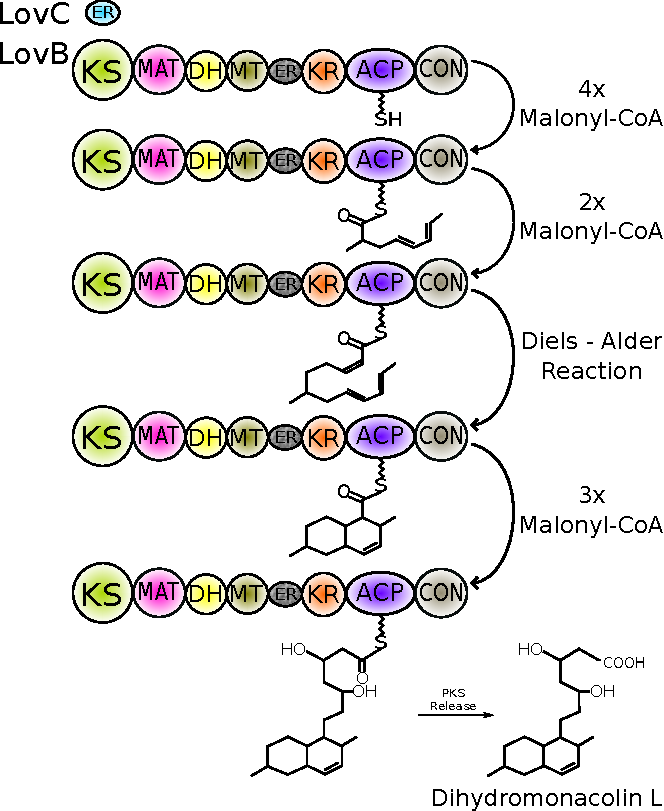
\includegraphics[width=0.7\textwidth, resolution=600, keepaspectratio=true]{graphics/lov.pdf}}
			\caption[A Type I polyketide synthase (iterative), the lovastatin system.]{ A Type I polyketide synthase (iterative), the lovastatin system. The figure here only shows the PKS LovB out of the two PKSs LovB and LovF utilized in the production of lovastatin. LovB is responsible for the production of dihydromonacolin L moiety which is produced by the iterative condensation of 9 malonyl-CoA extender unit. LovB carries a non functioning ER domain for which the function is substituted by LovC. The other domains in LovB consist of a ketosynthase, a malonyl transferase (MAT), a methyl transferase (MT), a dehydratases (DH), an enoyl reductases (ER), a ketoreductases (KR), an acyl carrier protein (ACP) and a condensation domain (CON).
			}
			\label{fig:lov}
			\end{figure}
			
			Another popular and well studied example is the type I iterative PKS that produces lovastatin, which is produced by the fungi \textit{Aspergillus terreus}. Lovastatin is a cholesterol lowering agent which acts as a precursor for the popular drug simvastatin. The lovastatin biosynthesis pathway consist of two PKSs LovB and LovF. LovB, which is responsible for the nonaketide moiety dihydromonacolin L, consists of a ketosynthase, a malonyl transferase (MAT), a methyl transferase (MT), a dehydratases (DH), an enoyl reductases (ER), a ketoreductases (KR), an acyl carrier protein (ACP) and a condensation domain (CON) (Figure \ref{fig:lov}). The ER domain in LovB is non functional therefore LovB utilizes a free standing ER LovC. LovB utilizes 9 malonyl-CoA extender units, a methyl donated from a S-adenosyl-L-methionine (SAM) molecule and an NADPH to produce dihydromonacolin L. LovF consists of all the above mentioned domains but it has a functional ER. LovF catalyses the formation of the 2-methylbutyrate moiety by the condensation of two acetyl units. Other enzymes encoded within the same gene cluster includes LovA and LovD. LovA encodes a cytochrome P450 oxygenase which oxidises the dihydormonacolin L produced by the LovB, which is covalently joined to the 2-methylbutyrate moiety by the trans esterase activity of the LovD. Figure \ref{fig:lov} shows the production of dihydromonacolin L by LovB and LovC in the lovastatin biosynthesis pathway, and includes  the proposed stage of a Diels-Alder reaction for ring formation in the growing polyketide \parencite{Kennedy1999,Ma2007, Campbell2010, Ames2012}. 
			
			Apart from the minimal PKS domains and one or more required \bet-keto processing domains, several type I PKS gene clusters contain a number of tailoring enzymes which perform further different functions at different stages of polyketide synthases. These tailoring enzymes may act on the ACP bound polyketide intermediate or on the released product post production. One such tailoring enzyme is 3-hydroxy-3-methyl glutryl-CoA synthase cassette (HCS) which is responsible for the \bet-branching in many type I PKS systems for example mupirocin, thiomarinol and kalimantacin \parencite{Haines2013}. The HCS cassette adds a methyl branch at the \bet-position of the growing polyketide chain by the coordinated action of five enzymes which include an ACP, an HMG-CoA synthase, two enzymes from the crotonase family and a decarboxylase. This \bet-methylation step is considered to be rate limiting and more complex as compared to the methylation of an $\alpha$ carbon by a methyl transferase. At the onset of \bet-methylation an ACP delivers a polyketide intermediate to the HMG-CoA domain in the HCS cassette. This delivery requires the ACP and the HMG-CoA from the HCS to interact and recognize each other at the appropriate stage of polyketide synthesis. At the time of starting my thesis, it was not very well understood what enables the HCS cassette to recognize the correct ACP for the \bet-branching. One of the projects in the present study was to explore the specificity mechanism of ACP-HCS interaction in the mupriocin pathway, which is described in Chapter \ref{cha:ACP-HCS}.
			
			Another recently discovered tailoring enzyme of interest is halogenase. In the curacin system this halogenase domain works in conjunction with the HCS proteins and is responsible for the addition of a chloride on the $\gamma$ carbon in the growing polyketide chain. In a study published by \textcite{Busche2012}, they found the recognition specificity between this halogenase domain and the ACP. Advances in PKS research are slowly unfolding the details of several different pathways, with a diversity of enzymes functioning in conjunction core PKS function. It is becoming increasingly interesting to understand structure function relationship of these auxiliary enzymes and to exploit them for synthetic biology purposes.
			
			\subsubsection{Type II PKS}
			\label{sec: typeIIPKS}
			Type II polyketide synthases produce aromatic compounds (polyphenols) in Gram-positive bacteria of the class actinomycetes, found in soil and marine environments. Some of the famous examples of type II polyketides are tetracyclines, which is a class of broad spectrum antibiotics, and doxorubicin, which is an anti cancer agent. In contrast to the type I PKSs, where all the catalytic domains are covalently bonded in a single polypeptide chain, the domains forming the type II PKS are encoded on separate genes. However, the genes encoding the type II domains are usually found to be clustered together. Type II PKSs utilize an acyl starter unit and a malonyl extender unit for Claisen condensation, using a single set of mono functional enzymes iteratively. A minimal set of a type II PKS domains comprises of two KSs, a KS$_{\alpha}$ and a KS$_{\beta}$ domain, and an ACP domain. Other catalytic domains such as ketoreductases and aromatases amongst others perform \bet-keto processing. It is much more difficult to study type II PKS as compared to type I PKS due to the very short span of stability of the intermediates produced. With type II PKS it is also not possible to predict the metabolites produced straight from the sequence of the biosynthetic domains involved, which is much simpler in type I modular PKS \parencite{Hertweck2007}. 

			\setlength\fboxsep{5pt}
			\setlength\fboxrule{1.5pt}
			\begin{sidewaysfigure} []
			\centering
			\fbox{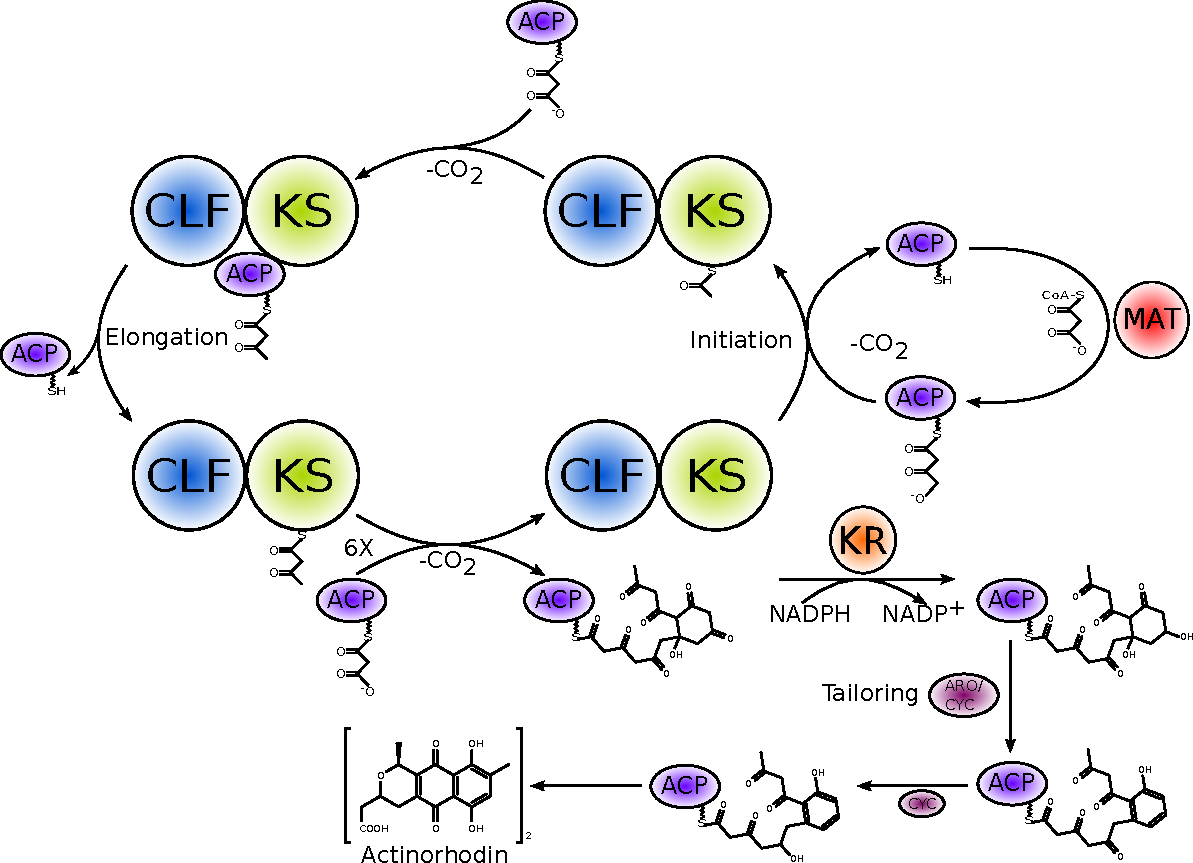
\includegraphics[width=0.7\textwidth, resolution=600, keepaspectratio=true]{graphics/actpathway.pdf}}
			\caption[Type II polyketide synthases from actinorhodin biosynthesis pathway]{Type II polyketide synthases from actinorhodin biosynthesis pathway. The chain length factor (CLF) and ketosynthase (KS) form a heterodimer. The malonyl-CoA:ACP transacylase (MAT) primes the ACP with the malonate unit. The biosynthesis begins with the decarboxylation of a malonyl unit on to the KS followed by the Claisen condensation with an activated malonyl unit. Overall 7 rounds of Claisen condensation takes place to reach the required length. Upon release the product undergoes post synthesis processing with aromatase and cyclase enzymes to produce actinorhodin molecule. Figure adapted from \parencite{Das2009}.}
			\label{fig:ACT}
			\end{sidewaysfigure}
						
			The KS$_{\alpha}$ and KS$_{\beta}$ domains form heterodimers, where KS$_{\alpha}$ is responsible for Claisen condensation and KS$_{\beta}$ keeps a check on the synthesized chain length, also known as \textquoteleft chain length factor\textquoteright (CLF). \nomenclature{CLF}{Chain length factor} KS$_{\beta}$ lacks a catalytic cysteine and therefore it can not perform Claisen condensation but upon mutating the position where a catalytic cysteine would be expected to a glutamine (KS$_Q $) it is capable of decarboxylating the malonyl unit into an acetate \parencite{Keatinge-Clay2004a}. This KS$_Q$ functionality is similar to the KS$_Q$s found in the modular type I PKS where they are utilized to convert a malonyl unit into an acetate starter unit \parencite{Bisang1999}. Swapping CLF from different type II PKS can result in the production of metabolites of different chain lengths.
			
			It is still not very well understood what catalyses the loading of a malonyl unit to the ACP of a type II PKS. Two alternative hypothesis were proposed both with similar possibility and experimental evidence. One hypothesis favours the self malonylation of the ACP, which was experimentally verified \textit{in vitro} in a purified sample of type II PKS \parencite{Arthur2005}. The other hypothesis argues a potential involvement of a malonyl-CoA:ACP transacylase  (MAT) but most of the type II PKS cluster lacks an MAT therefore it was hypothesized that this MAT is borrowed from a FAS in the cell \parencite{Dreier1999,Keatinge-Clay2003}. Type II PKS are also found to utilize domains such as KR, DH and ER from the host FAS \parencite{Tang2006a}. 
						
			Figure \ref{fig:ACT} summarizes the biosynthetic pathway of the type II antibiotic actinorhodin produced by \textit{Streptomyces coelicolor} as an example of a type II PKS. Actinorhodin biosynthesis initiates by the priming of the malonate unit onto an ACP by the malonyl-CoA transacylase. The malonyl-CoA unit is decarboxylated and transferred to the cysteine thiol of the KS$_{\alpha}$ which acts as the starter unit. This step is followed by seven iterative Claisen condensation cycles. At the end of the condensation cycles the intermediate product undergoes keto reduction and successive aromatization and cyclization to produce the polycyclic end product actinorhodin. Actinorhodin biosynthesis is carried out purely by  a minimal set of type II  PKS followed by downstream processing with tailoring enzymes however, other secondary metabolites like R1128 and doxurubicin require an initiation module to produce a diketide starter unit prior to the minimal type II PKS activity. This initiation module consists of a KS homodimer and an ACP, the absence of the CLF suggests the non requirement of chain length control in this module. Further details, including a cartoon representation of an initiation module, are given elsewhere \parencite{Das2009}.
			
			\subsubsection{Type III PKS}
			\label{sec: typeIIIPKS}

			\setlength\fboxsep{5pt}
			\setlength\fboxrule{1.5pt}
			\begin{sidewaysfigure} []
			\centering
			\fbox{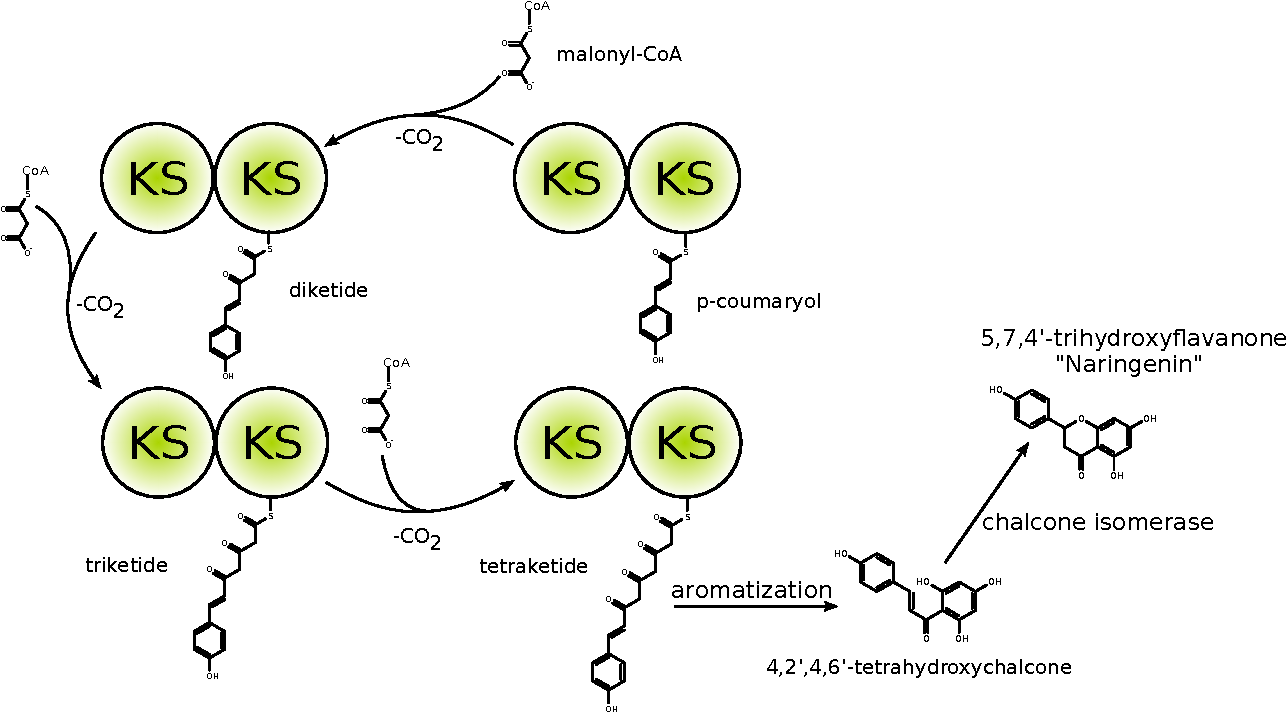
\includegraphics[width=\textwidth, resolution=600, keepaspectratio=true]{graphics/chs.pdf}}
			\caption[Proposed reaction mechanism of Type III polyketide synthases/Chalcone synthase]{Proposed reaction mechanism of Type III polyketide synthases/Chalcone synthase. The growing metabolite is shown attached to one of the KS of the homodimer. The p-coumarocyl-CoA starter unit is condensed iteratively with three acetate units derived from malonyl-CoA, followed by aromatization and chalcone isomerization to produce Naringenin. Figure adapted from \parencite{Ferrer1999}.}
			\label{fig:CHS}
			\end{sidewaysfigure}
						
			Type III PKS commonly found in plants, but with recent discoveries in bacterial systems as well, belong to the superfamily of chalcone synthases (CHS) \nomenclature{CHS}{Chalcone synthases} / stilbene synthases (STS) \nomenclature{STS}{Stilbene synthases}. CHS is the first step in the plant flavanoid biosynthesis and is responsible for a variety of plant metabolites, with functions including defence, pigmentation and fertility.  CHSs utilizes a single homodimeric ketosynthase iteratively, catalyses Claisen condensation of a p-coumaroyl-CoA, as a starter unit, to the three acetate units derived from malonyl-CoA. The same catalytic centre is also further utilized for successive aromatization and cyclization to produce chalcone. Figure \ref{fig:CHS} explains the chalcone biosynthetic pathway proposed by \textcite{Ferrer1999}. PKS type III represents a divergent class of this CHS functionality with the diversity in the choice of starter units, extender units, number of chain extensions and subsequent cyclization. There were differences found in the bacterial and plant type III PKSs, for example bacterial type III PKS can utilize an acyl-ACP starter unit by involving an ACP from an FAS, whereas plants use acyl-CoA as the starter unit. Based on structural analysis of the type III PKS ketosynthase \textcite{Qiu2001a} have suggested the emergence of these enzymes from the fatty acid KAS III. FAS KAS III are responsible for the initiation of type II FAS biosynthesis. The type III PKS utilizes CoA thioesters instead of a phosphopantetheinylated ACP to tether the growing polyketide product \parencite{Austin2003}. 
			
		\subsection{PKS domains}
			\subsubsection{Acyl carrier protein (ACP)}
			\label{sec: ACP}
			Acyl carrier proteins (ACP) belong to a class of carrier proteins which are involved in channelling the substrates via a phosphopantetheine prosthetic group. These carrier proteins are known to be involved in fatty acid synthesis (FAS), polyketide synthesis (PKS) and non-ribosomal peptide synthesis (NRPS) \nomenclature{NRPS}{Non Ribosomal Peptide Synthase}. The carrier proteins involved in FAS and PKSs are called ACPs, but peptidyl carrier proteins (PCP) \nomenclature{PCP}{Peptidyl Carrier Proteins} in NRPSs. In FAS the same ACP domain is utilized iteratively to pass the substrate to the different domains of the module multiple times whereas in PKSs, especially in type I modular PKS, each module has its cognate ACP to perform the substrate channelling for that module. Although the carrier proteins share a wide range of sequence identity among various organisms, they still share a common structural fold. A sequence identity of \textgreater80\% is reported between ACPs from \textit{E. coli} and \textit{V. harveyi}, whereas 21\%-27\% sequence identity between \textit{E. coli} and rat ACPs \parencite{Byers2007}.  A common carrier protein fold consists of a 4 helical bundle which ranges from 70 to 100 amino acids long. Among the three major $\alpha$ helices, helix I runs antiparallel to helix II and IV with a small helix III which runs almost perpendicular to the axis of the three major helices. Inspite of their small structure carrier proteins are found to exhibit great degree of plasticity in their backbone movement. FAS ACPs are found to sequester the growing fatty acid chain within the hydrophobic pocket in the centre of ACP \parencite{Chan2008}. On the other hand NRPS PCPs have been shown to be involved in backbone rearrangement and helical movement during substrate chanelling \parencite{Koglin2006}. However, no such intrinsic conformational motion has yet been reported in PKS ACPs, which is discussed in more detail in Chapter \ref{cha:chap5}. These carrier proteins are translated as inactive apo proteins that are activated by addition of the 4\textquoteright-phosphopantetheine moiety of a coenzyme A, through the action of 4\textquoteright-phosphopanthetheine transferase \parencite{Mootz2001}. This 4\textquoteright-phosphopantetheine moiety is attached to a conserved serine at the end of the helix II via a phosphodiester bond (see Figure \ref{fig:acp}). Carrier proteins have also been found to be abundant in various organisms, with 80 reported in \textit{Streptomyces avermitillis}.
					
			In a typical PKS pathway an ACP has to interact with a large number of proteins which include 
			\begin{inparaenum}[\itshape 1\upshape)]
			\item an AT domain, either \textit{cis} or \textit{trans} 
			\item an upstream KS domain 
			\item a downstream KS domain 
			\item other catalytic domains for example KR, DH, ER, and
			\item several other tailoring enzymes. 
			\end{inparaenum}
			Until recently it was not known how the relatively small structure of the carrier proteins interact with such a diverse set of interacting partners. There were several unanswered questions such as, how much of the carrier protein\textquoteright s surface interacts with the partner protein? Does each interaction occur at a different face of the protein? What drives the phosphopantetheine arm to the different catalytic domains? Some of these questions have been answered lately however, there is still a lot to be discovered. 

			
			\setlength\fboxsep{5pt}
			\setlength\fboxrule{1.5pt}
			\begin{figure} []
			\centering
			\fbox{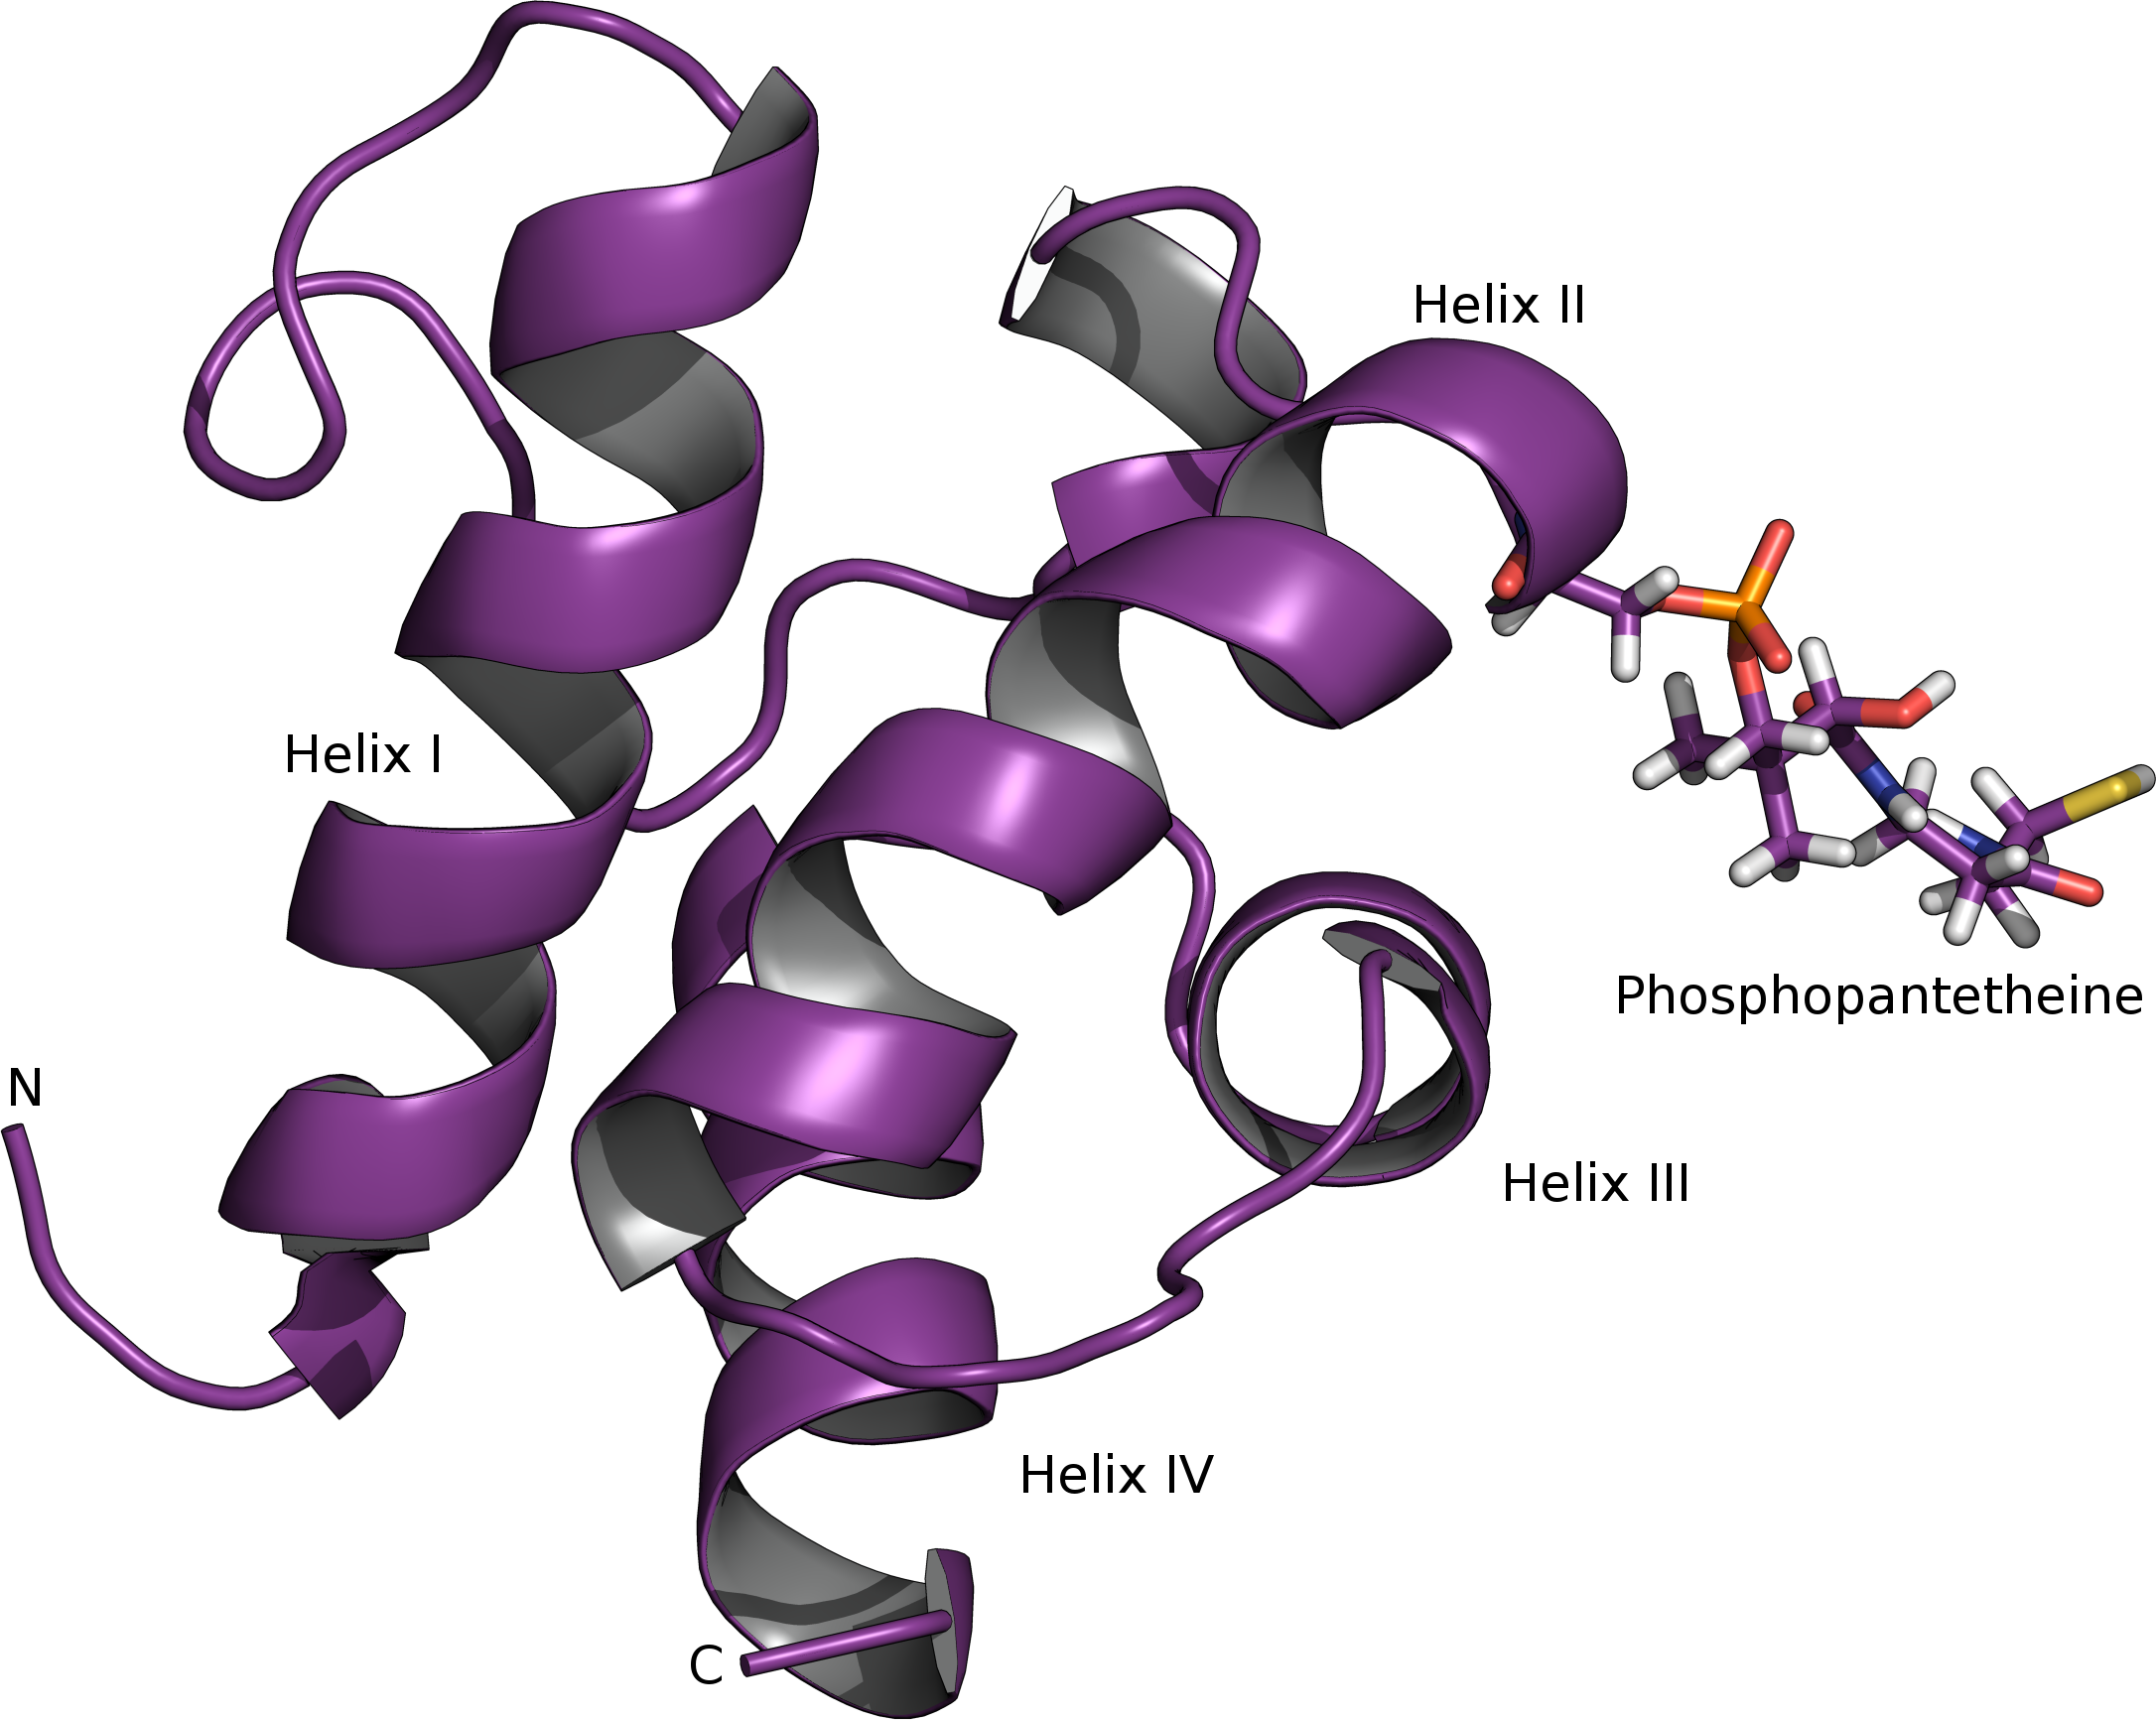
\includegraphics[width=\textwidth, resolution=600, keepaspectratio=true]{graphics/acp.png}}
			\caption[Cartoon representation of an acyl carrier protein from mupirocin pathway]{Cartoon representation of an acyl carrier protein (ACP-A3a) from the mupirocin biosynthesis pathway (PDB ID 2L22). A phosphopantetheine arm is modelled attached to the catalytic serine, represented as sticks \parencite{Haines2013}. }
			\label{fig:acp}
			\end{figure}
			
			
			In a study of FAS ACPs by \textcite{Zhang2003} helix II was shown to interact with various interacting partners as the \textquotedblleft recognition helix\textquotedblright. Helix II being conserved and negatively charged interacts with the positively charged channels of various ACP dependent proteins \parencite{Zhang2001}. However, studies by Khosla's group of PKSs have shown by structural modelling and mutagenesis work that loop I and helix I are the interacting interface for the chain elongation and translocation steps respectively. In another study on curacin biosynthesis helix III on the ACP was found to be interacting with and the halogenase enzyme \parencite{Busche2012}. In the present work as well, helix III is shown to be one of the anchors that interacts with  MupH, as described in Chapter \ref{cha:ACP-HCS}. Thus, it can be said that helix II, which was considered to be the \textquotedblleft recognition helix\textquotedblright, is not the only surface with which ACPs interact with other proteins. Further exploration may lead to finding some other novel features not yet discovered.
			
			Till now there are only 6 entries in the PDB representing 4 different structures solved for the ACPs from PKS systems, 2 for each \textit{cis} and \textit{trans} AT systems. The first set of structures for the \textit{cis} AT PKS were published in 2007 from module 2 of the DEBS system (PDB ID 2JU1, 2JU2) \parencite{Alekseyev2007}, followed by the structure of ACP1 from the CurA module of curacin system (PDB ID 2LIU, 2LIQ) in 2012 \parencite{Busche2012}. Structures from the trans AT systems came out very recently in 2013 for the didomain ACP in the MmpA subunit of the mupriocin system which are involved in \bet-branching mechanism (PDB ID 2L22) \parencite{Haines2013} followed by the solution structure of ACP 5 from the virginiamycin cluster (PDB ID 4CA3) in early 2014 \parencite{Davison2014}.
			
			\subsubsection{Acyl transferases (AT)}
			\label{sec:AT}
			In PKS and FAS systems acyl transferase domains are responsible for loading the starter and extender units onto the ACPs. In the type I modular PKS systems the AT domains can either be covalently bound in the same polypeptide chain, which are called \textit{cis} AT e.g. as in erythromycin synthesis, or can exist in \textit{trans} as discrete domains e.g as in mupirocin synthesis. In FAS systems, the acetyl starter and malonyl extender moiety are transferred on to the same AT domain, at different times, via acetyl/malonyl transferase from an acetyl-CoA/malonyl-CoA molecule. Thus, an FAS AT domain has dual specificity for the starter and extender units and there is a competition between the two substrates for the AT active site. This phenomenon also holds in many \textit{trans} AT PKS systems, for example mupirocin, where a single set of AT domains is responsible for loading both the starter and the extender units. On the other hand, \textit{cis} AT PKS systems have a separate module for loading the starter unit and the AT domain that is covalently bound to a particular module allows loading its cognate extender unit. Thus in principle AT domains can have specificity towards their own extender units allowing different extender units to be utilized at each elongation step \parencite{Khosla1999}. 
			
			The AT domain catalyses the starter and extender unit's transfer from a  CoA on to the phosphopantetheine of an ACP. This transfer is achieved by a ping-pong bi-bi reaction mechanism utilizing a conserved SER-HIS diad (e.g. S642 and H745 in DEBS AT5). The malonyl or methyl malonyl moiety was found to interact with the conserved active site ARG (e.g. R667 in DEBS AT5) at the beginning of the reaction \parencite{Tang2006}. The catalytic SER resides in  a highly conserved motif, GHSXG, and is responsible for the nucleophilic attack on the carbonyl of the acyl moiety offered by the CoA. This nucleophilic attack leads to the formation of a SER-acyl tetrahedral geometry, which is hypothesized to be stabilized by an oxyanion hole formed by the backbone amides (e.g. Q9 and V98 in S. coelicolor MAT structure), and to the release of CoA \parencite{Keatinge-Clay2003}. HIS in the diad helps to enhance the nucleophilicity of the SER. In the second step of the reaction the thiol of the incoming phosphopantetheine initiates a nucliophilic attack on the SER bound acyl carbonyl forming SER-acyl-ACP tetrahedral intermediate which is released by the protonation of the active site SER by the active site HIS (Figure \ref{fig:ATreact}) \parencite{Tsai2009, Dunn2013}. 
			
			Figure \ref{fig:AT} shows the cartoon structure of an AT domain from the module 5 of the DEBS system and the proposed reaction mechanism is shown in Figure \ref{fig:ATreact}. AT domains follow  an $\alpha$/$\beta$-hydrolase fold as the core catalytic domain of approx 240 residues attached to a smaller ferredoxin like  domain of approx 60 residues. The N-terminus of the AT domains in the \textit{cis}-AT systems are found to contribute to the KS-AT linker (approx 140 residues) which is termed equivalent to the docking domain in the \textit{trans}-AT systems \parencite{Tang2006, Gay2014}. However, the docking domain in the \textit{trans}-AT systems does not carry any portion of the AT domain but is formed by the linker sequence in between the KS and the subsequence domain \parencite{Gay2014}. This linker region in the \textit{cis} system (DEBS) is found to be important for the interaction of the ACP during chain transfer and elongation \parencite{Kapur2010, Kapur2012}. Although the crystal structure of a docking domain attached to the KS in the trans AT system was recently published the role of the docking domains are still not understood \parencite{Gay2014}. 
			
			\setlength\fboxsep{5pt}
			\setlength\fboxrule{1.5pt}
			\begin{sidewaysfigure} []
			\centering
			\fbox{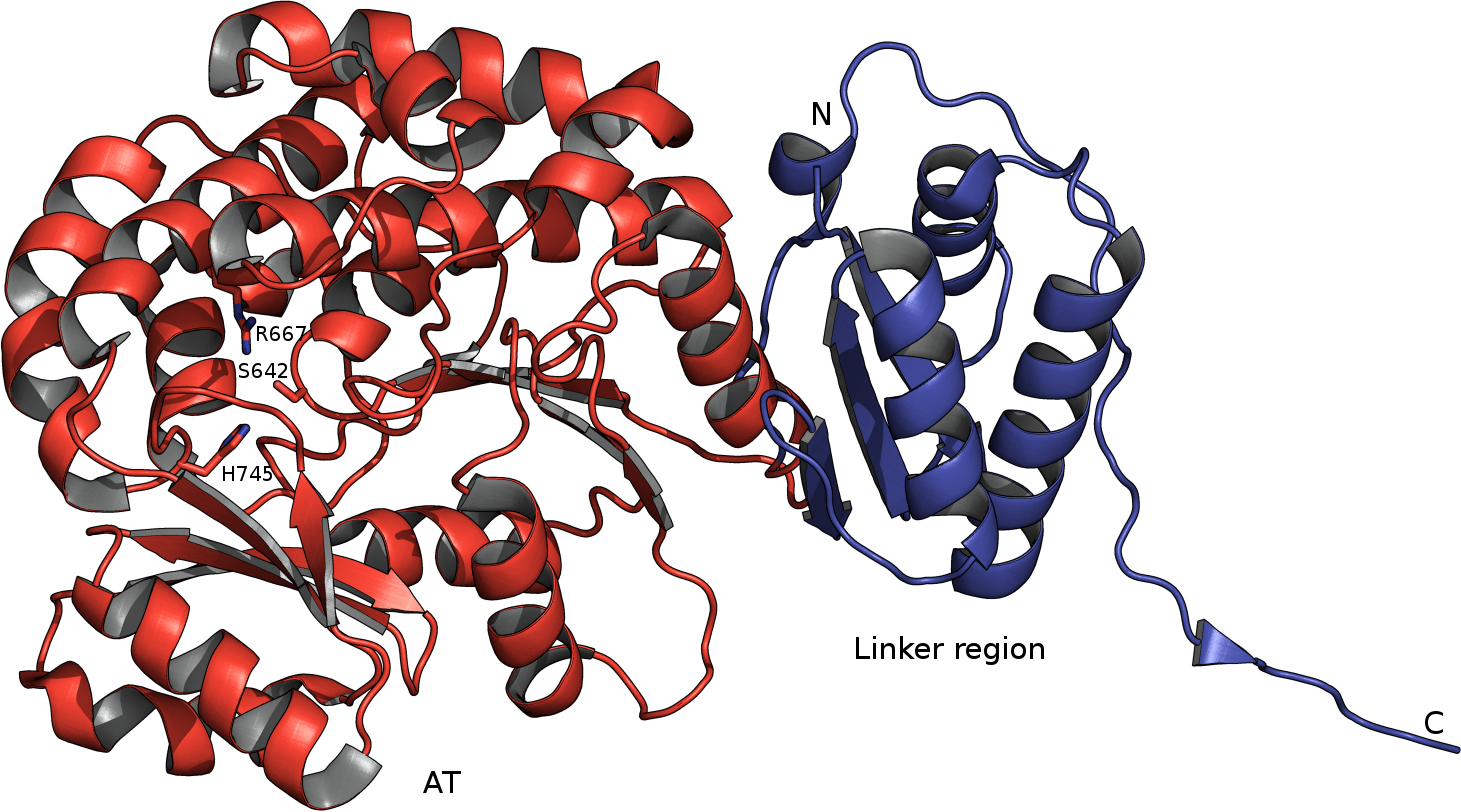
\includegraphics[width=\textwidth, keepaspectratio=true]{graphics/at.png}}
			\caption[Cartoon representation of an acyl transferase domain from the module 5 of DEBS system]{Cartoon representation of an acyl transferase domain (red) from the module 5 of DEBS system along with the linker region (blue) between the KS and the AT domains (PDB ID 2HG4). The catalytic diad S642 and H745 are drawn as sticks along with the conserved active site R667 \parencite{Tang2006}. }
			\label{fig:AT}
			\end{sidewaysfigure}			
			
			\setlength\fboxsep{5pt}
			\setlength\fboxrule{1.5pt}
			\begin{figure} []
			\centering
			\fbox{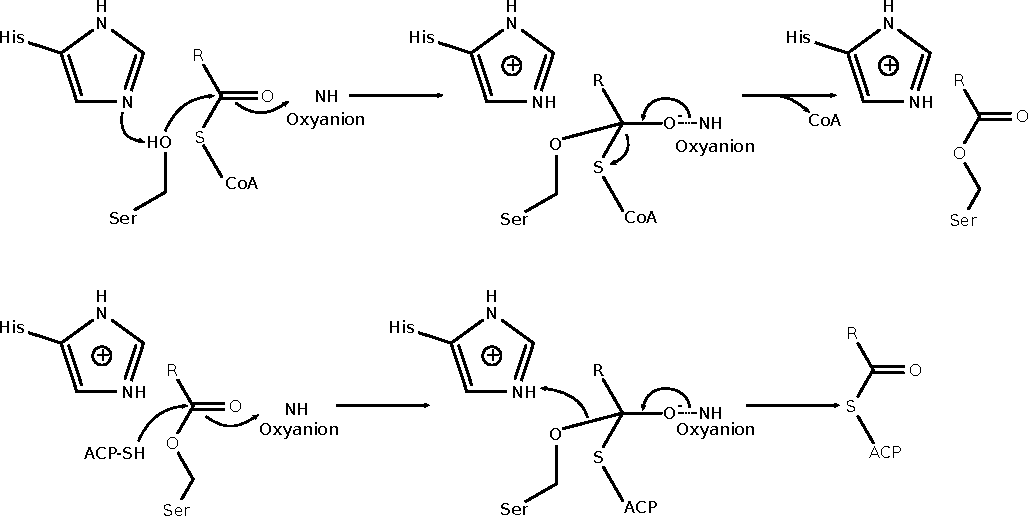
\includegraphics[width=0.95\textwidth, resolution=600, keepaspectratio=true]{graphics/ATreact.pdf}}
			\caption[Proposed reaction mechanism of AT domain]{Proposed reaction mechanism of AT domain. Figure adapted from \parencite{Smith2007}.}
			\label{fig:ATreact}
			\end{figure}
			
			Although the ATs from type I and II PKS and FAS share the same catalytic reaction mechanism and protein fold exhibit a wide range of tolerance and specificity towards the starter and extender units they transfer on the ACP. \textit{In silico} and mutagenesis experiments have identified conserved motifs within the vicinity of active site serine which determines the specificity towards the different substrates. The loading domains in the \textit{cis}-AT systems were found to have more tolerance for a greater variety of starter units such as acetyl, propionyl, isopropionyl than the AT domains responsible for loading the extender units such as malonyl and methyl manlonyl \parencite{Lau1999a,Liou2003}. 
			
			The X in the GHSXG motif, which is usually a branched amino acid such as valine or isoleucine in the malonyl specific ATs, is either a glutamine or methionine in the methyl malonyl specific ATs \parencite{Haydock1995}. On comparing AT structures from DEBS AT5 with a mammalian FAS AT, DEBS AT5 has a glutamine at the X position which makes it specific for methyl malonyl extender unit, whereas mammalian FAS AT has a valine or leucine at the X position which makes it specific for malonyl extender unit \parencite{Tang2006}. 
			
			In another study, \textcite{Yadav2003} studied 187 AT sequences from 19 type I modular PKS clusters and predicted motif QQ\textbf{GHS[QMI]G}RSHT[NS]V was responsible to confer specificity towards methyl malonyl substrate and QQ\textbf{GHS[LVIFAM]G}R[FP]H[ANTGEDS][NHQ]V motif was associated with malonyl specificity. They have also identified a position R117 in \textit{E. coli} malonyl-CoA:acyl carrier protein transacylase crystal structure (PDB ID 1MLA) which was conserved in all the malonyl and methyl malonyl specific ATs but changes to a non polar amino acid for the ATs specific for monocarboxylic substrates such as propionate. These motifs are embedded in their PKS domain detection program SEARCHPKS \parencite{Yadav2003a}. Another motif is the YASH motif which contains the catalytic histidine 100 residues downstream of the catalytic serine. YASH motif was found to be specific in the methyl malonyl specific ATs whereas HAFH at the same position was specific for the malonyl substrates \parencite{Haydock1995}.  
			
			\subsubsection{Ketosynthases (KS)}
			\label{sec:KS}			
			Ketosynthases are responsible for catalysing Claisen condensation in PKS, FAS and NRPS systems. KSs belong to the thiolase family of proteins and in type I FAS and type I and III PKS they form homodimers \parencite{Austin2003, Tang2006}. KSs in type II PKS also forms the dimer but only one subunit performs the Claisen condensation and the second subunit which is also known as chain length factor is a non functional KS considered to be responsible for keeping a check on the growing polyketide chain length \parencite{Tang2003, Szu2011}. The homodimeric state in type I PKS and FAS is considered to be the primary factor for the dimerization of the two subunits. Although ER and DH domains are also found to form dimers, experiments have shown that upon KS deletion the FAS subunits fails to dimerize \parencite{Smith2007}. The thiolase fold of the two dimer forming KSs follow the same  alternating $\alpha /\beta/ \alpha/ \beta/ \alpha$ architecture. The active site is formed at the dimer interface by the contribution of the residues from both the subunits. The active site can be viewed as two segments, one at the most buried segment is next to the dimer interface and bind the acyl intermediate, and an outer tunnel starts from the enzyme surface and binds the phosphopantetheine arm. Sequence analysis has shown diversity and lesser sequence similarity in the residues lining the acyl intermediate binding pocket as compared to the phosphopantetheine binding tunnel \parencite{Olsen2001}. This is due to the ability of the KS across different systems to accept a variety of substrates which are however, attached to the same phosphopantetheine arm. 
			
			There are two main classes of Claisen condensations for carbon-carbon bond formation; the decarboxylating and the non-decarboxylating. The structures of the KSs used for both the classes are low in sequence similarity but still have the same three dimensional thiolase fold \parencite{Heath2002}. The decarboxylating condensing enzymes can be further divided into two sub classes based on the primary sequence analysis 1) Initiation ketosynthase such as type I FAS, FabH  and 2) Elongation ketosynthases such as type I FAS, FabB and FabF \parencite{Davies2000}. The initiation enzymes utilize CoA substrate as the primer whereas the elongation enzymes utilize ACP thioesters however, the reaction mechanism followed by both the enzymes is same. The initiation ketosynthases as the name suggests are found at the beginning of the type I FAS and PKS usually in the loading module for example the niddamycin pathway \parencite{Kakavas1997}.
			
			After years of disagreement and research and with the availability of the high resolution crystal structures of KSs from both FAS and PKS systems researchers have come to the consensus that the Claisen condensation is a three step process involving a CYS-HIS-HIS catalytic triad (Figure \ref{fig:KSreact}). In the \textit{E. coli} FAS (FabB/FabF) KS (PDB ID 1DD8) C163, H298 and, H333 forms the catalytic triad (Figure \ref{fig:KS}). The Claisen condensation initiates with the acyl chain transfer from an ACP on to the catalytic cysteine forming an ACP-acyl-KS thioester tetrahedral intermediate. In FAS (FabB/FabF) this tetrahedral geometry is stabilized by the backbone amides contributed by the catalytic cysteine and a glycine (G391). The pKa of a free cysteine (8.0 to 8.8) is not sufficient for the deprotonation and the nucleophilic attack on the acyl carbonyl. A pKa of about 7.0 or lower is required for the cysteine to act as a nucleophile under physiological conditions. \textcite{Qiu1999} suggested H244 may be involved in assisting the deprotonation of the cysteine thiol. However the distance between the N $\epsilon$ ans S $\gamma$ of the H244 and catalytic cysteine respectively were too far for this to happen. Furthermore replacement of H244 with an alanine resulted in a protein that was unable to catalyse the complete condensation reaction, but was 6 times faster in transacylation than the wild type. However, mutagenesis studies on H244 do show that it assists in the deprotonation of the thiol at low pH \parencite{Davies2000}. The probable explanation for the deprotonation of the catalytic cysteine thiol under physiological conditions was given on the basis that the cysteine is present at the N-terminus of the alpha helix, the positive end of the dipole moment of the helix could stabilize the negative charge, allowing transfer to the acyl chain to the cysteine \parencite{Davies2000}.

			\setlength\fboxsep{5pt}
			\setlength\fboxrule{1.5pt}
			\begin{figure} []
			\centering
			\fbox{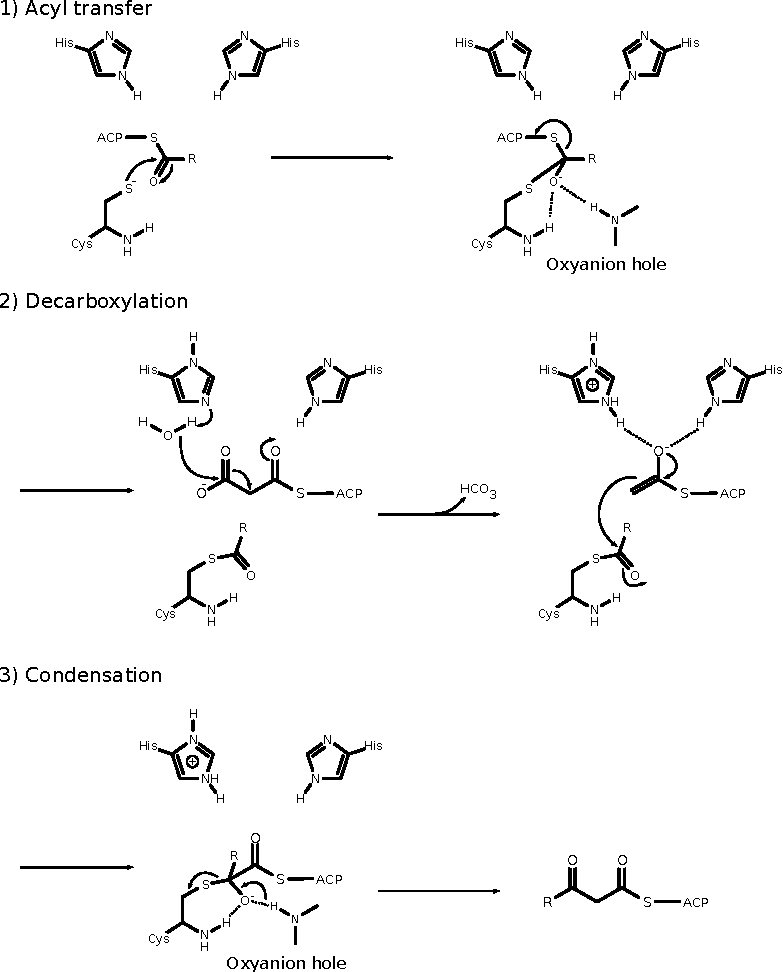
\includegraphics[width=0.95\textwidth, resolution=600, keepaspectratio=true]{graphics/KSreact.pdf}}
			\caption[Proposed reaction mechanism for Claisen condensation]{Proposed reaction mechanism for Claisen condensation. Figure adapted from \parencite{Smith2007}.}
			\label{fig:KSreact}
			\end{figure}			
						
			\setlength\fboxsep{5pt}
			\setlength\fboxrule{1.5pt}
			\begin{sidewaysfigure} []
			\centering
			\fbox{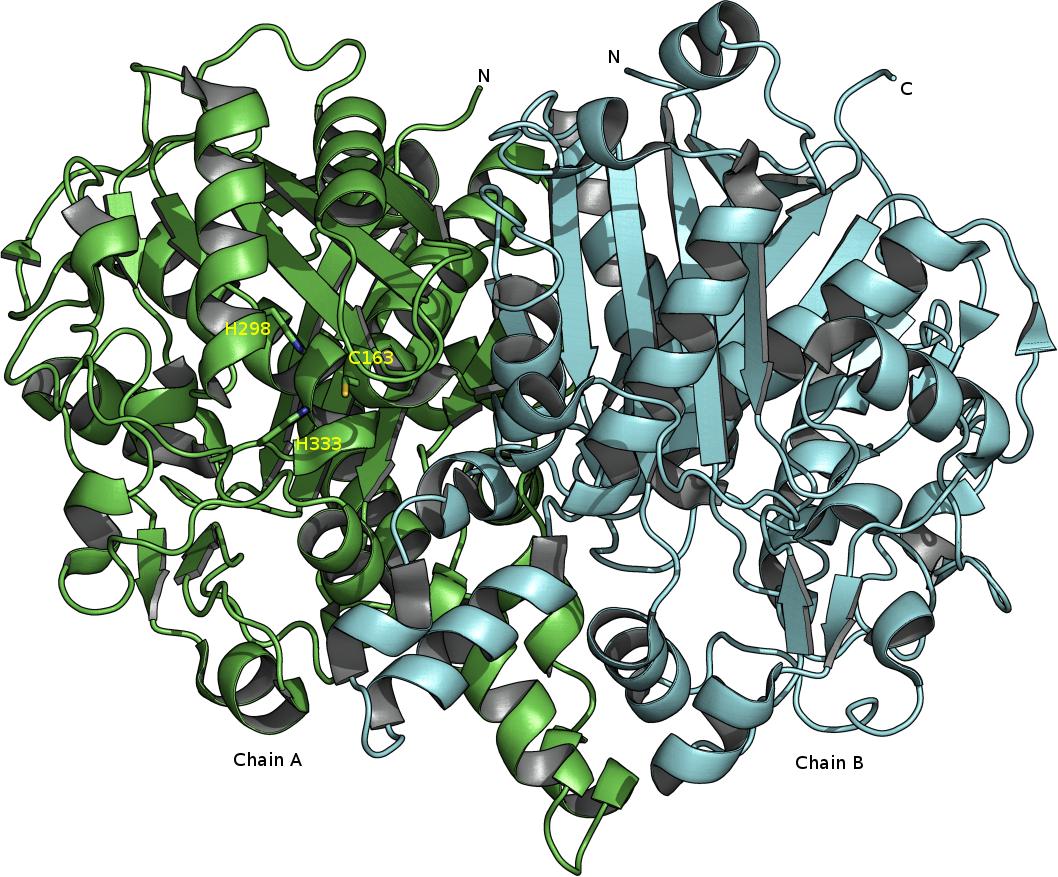
\includegraphics[width=0.7\textwidth, keepaspectratio=true]{graphics/ks.png}}
			\caption[Cartoon representation of a ketosynthase homo dimer from FAS in \textit{E. coli}]{Cartoon representation of a ketosynthase homo dimer from FAS in \textit{E. coli} (PDB ID 1DD8). The catalytic triad C163, H298 and H333 are drawn as sticks \parencite{Olsen1999}.}
			\label{fig:KS}
			\end{sidewaysfigure}
			
			The second step involves the decarboxylation of the malonyl extender unit attached to the ACP. The two histidines are considered to be involved in the decarboxylation of the malonyl unit. A water molecule in the active site is thought to be activated by one of the histidines which in turn attacks the C3 carbonyl of the malonyl resulting in the formation of an enol intermediate, stabilized by the histidines. This decarboxylation step also happens in the absence of the acyl-cysteine thio ester and that is why the above mentioned initiation keosynthases that lacks catalytic cysteine are able to decarboxylate a malonyl or methylmalonyl units into an acetyl or propionyl units respectively. Such initiation ketosynthases carry a glutamine in place of a cysteine (also known as $ KS^{Q} $). In the final step the enol intermediate forms a carbanion which in turn attacks the acyl-cysteine thio ester resulting in a tetrahedral intermediate which is again stabilized by the oxyanion hole followed by the release of the acyl-ACP \parencite{Heath2002}. 
			
			In modular \textit{cis}-AT PKS, Ketosynthases have shown to be tolerant in terms of substrate specificity and can readily accept non native substrates. Studying the structure of the type I and type II KS, type I KSs have a loop at the interface in the homodimers which is replaced by a helix in the type II KSs. This loop region is hypothesized to be responsible for providing additional space to accommodate non native substrate which otherwise is restricted by the helix in the type II KSs \parencite{Pan2002}. KSs were able to catalyse chain elongation with inactivated KR5 or ER4 domain in the DEBS system. KS2 in the DEBS system was also found to be tolerant towards several substrates \parencite{Khosla1999}. Using a KS1 knockout strain  \textcite{Khosla1999} showed that (2S,3R)-diketide  and analogous substrates attached to a NAC molecule tolerated and processed by the KS2 domain. Not only different variants of diketide moeities they also tested an anhydro-triketide moiety which was able to be processed by the KS2, these substrate variants produced analogues of 6-DEB molecule. As well as KS2 being tolerant towards (2S,3R)-diketide moiety KS3, KS5 and KS6 were also able to accept and produce triketide products \parencite{Khosla1999}. 
			
			Recent phylogenetic studies have shown that the \textit{cis} and \textit{trans} PKS evolved independently through different routes. The KS from the \textit{trans}-AT systems were likely to be incorporated via horizontal gene transfer as opposed to gene duplication events in the \textit{cis}-AT systems. This difference may explain how \textit{trans} AT systems came to be more specific towards their substrates as compared to their \textit{cis}-AT counterparts \parencite{Nguyen2008}. These hypothesis were also experimentally supported by the two recent collaborative papers by Piel and Oldham group. In the first paper by \textcite{Jenner2013} utilizing a newly developed mass spectrometry (MS) based method to study ketosynthases specificity analysed substrate specificity of KS5 from bacillaene and KS1, KS2 and KS3$^{0}$  from psymberin biosynthesis pathways. KS5 in the BaeL subunit resides right before the key \bet-branching step which naturally makes it tolerant for non branched substrates. Similarly KS1 and KS2 from PsyA processes non branched substrate and KS3$^{0}$ from PsyD is a non condensing keto synthase but is capable of acyl transfer. \textcite{Jenner2013} incubated these ketosynthases with different SNAC analogues containing branched and unbranched substrates and tested their ability to produce product with MS. They found that the KS5 from BaeL and KS3$^{0}$ from PsyD do not tolerate branched substrate however were able to successfully process unbranched substrates. On the other hand KS1 and KS2 from PsyA were able to process branched substrate with lowered specificity. Upon sequence analysis, homology modelling and substrate docking of KS5 of BaeL, they found that the residue right before the catalytic cysteine (X-cys) seems to interact with the \bet-carbon. This position X is usually a bulky residue like methionine in the non branch accepting ketosynthases and a smaller residue like glycine or alanine in the branched chain accepting ketosynthases. KS5 from BaeL and KS3$^{0}$ from PsyD  have methionine on that position whereas KS1 and KS2 form PsyA have an alanine, which explains the more tolerant behaviour of the branched substrate by KS1 and KS2. To test this prediction from the computational analysis \textcite{Jenner2013} created a KS5 M237A mutant and incubated it with branched and unbranched SNAC analogues. The unbranched analogues were successfully transferred onto the catalytic cysteine of the KS5 mutant as the more space created inside the active site would have not affected the binding of the unbranched substrate. However, the KS3 mutant also showed increased levels of branched substrate specificity which suggests the necessity of the space created by replacing a bulky residue with a small residue immediately preceding the catalytic cysteine. These experiments laid down the new rules for predicting the specificity of KS domains towards branched and unbranched substrates. Although this rule is only restricted to the \bet- position in the substrates authors do not deny the possibility of discrimination based on the interactions at other parts of the substrate. 
			
			In the second paper, \textcite{Kohlhaas2013} tested the specificity of the bacillaene system KS1 domain from BaeJ for amino acid derived intermediates using the same protocols as mentioned above. KS1 in BaeJ accepts a glycine derived substrate from an upstream NPRS module, to test the tolerance of KS1 for different amino acid based substrates \textcite{Kohlhaas2013} created several different full length acyl-SNAC analogues utilizing glycine, alanine and valine to generate 2-amido variants. Upon incubating KS1 with the three 2-amido variants, the glycine derived substrate was able to readily transfer to the KS1 whereas the alanine based substrate did so with lower efficiency. The substrate based on valine failed to acylate KS1. In order to accommodate the bulkier valine derived substrate \textcite{Kohlhaas2013} identified M268 and L450 as the likely residues that offer steric hindrance in the entry of the substrate. They created two mutants M268A and L450A and tested all the three amino acid derived substrates. Glycine and alanine variants were still able to acylate however, the valine variant couldn't. These differences in the acylation efficiency suggested the intrinsic incompatibility of the groups at the $ \alpha $ position. They also created SNAC analogues to test any long range interaction beyond the \bet-position in the intermediates and the affect of not incorporating amide from an $ \alpha $ amino acid. There were no acylation observed in the substrate created to test the long range interaction as well as for the amide from the non $ \alpha $ amino acid. Two other acyl-SNAC analogues featuring 2-amino and 4-keto groups were also incubated to test for acylation efficiency. 2-amino SNAC  was able to acylate efficiently however, no observable acylation occurred with a 4-keto SNAC substrate. These observations suggested the need for an NH at the 2nd position, which would act as an efficient hydrogen bond donor, and that there is no requirement of the 4th carbonyl for the successful acylation. 
			
			\textcite{Kohlhaas2013} also tested KS1 for the effect of different residue type N-terminal to the catalytic cysteine on KS1's ability to accept different substrates. Through sequence analysis they found that most of the amino acid accepting KSs posses an asparagine residue at the position before the catalytic cysteine along with a few occurrence of alanine. On comparing with other ketosynthases in either \textit{cis} or \textit{trans}-AT systems they could never find an asparagine at that position. The dominating presence of an asparagine residue suggested its likely involvement in the acylation of the 2-amidoacetly substrate to KS1. To test this hypothesis they created an N206A mutant and incubated with 2-amidoacetly-SNAC. The mutant strain showed much lowered acylation efficiency. 
			
			\subsubsection{Ketoreductases (KR)}
			\label{sec:KR} 
			Ketoreductases are enzymes responsible for reducing the \bet-keto group to hydroxyl in FAS and PKS systems with the involvement of NADPH as the reducing agent. Unlike KSs which need to exist as a homodimers to function, KRs exist as functional monomers in the PKS dimer. KRs are thought to be responsible for the formation of most of the chiral centres in Polyketide products. 
			
			The stereo specificity of the products of KR domains was verified through domain swapping experiments with the KR2 from the DEBS system and the KR2 from the rapamycin system. The KR2 in the DEBS system produces an L-\bet-hydroxyl group whereas the KR2 from the rapamycin system is responsible for a D-\bet-hydroxyl group. In a model system using DEBS1 (Figure \ref{fig:DEBS}) and the DEBS thioesterase, domain swaps from rapamycin KR2 to DEBS KR2 produced a triketide with a D-\bet-hydroxyl group, confirming the stereo specificity of the KS product \parencite{Cortes1995}. It should also be noted that the mammalian FAS are known to produce D-\bet-hydroxyl groups whereas DEBS KRs produce an L-\bet-hydroxyl group, this observation also suggests that the KRs are not only responsible for the \bet-keto reduction but also for assigning the correct stereo chemistry to the resultant hydroxyl group \parencite{Kao1998}. KRs from the DEBS systems were also found to be tolerant of different substrates. In a domain swap experiment, a system with KR5 from the DEBS system replacing KR2 successfully produced the DEBS1 triketide product, suggesting a wide tolerance for KR substrate specificity \parencite{Khosla1999}.
			
			\setlength\fboxsep{5pt}
			\setlength\fboxrule{1.5pt}
			\begin{sidewaysfigure} []
			\centering
			\fbox{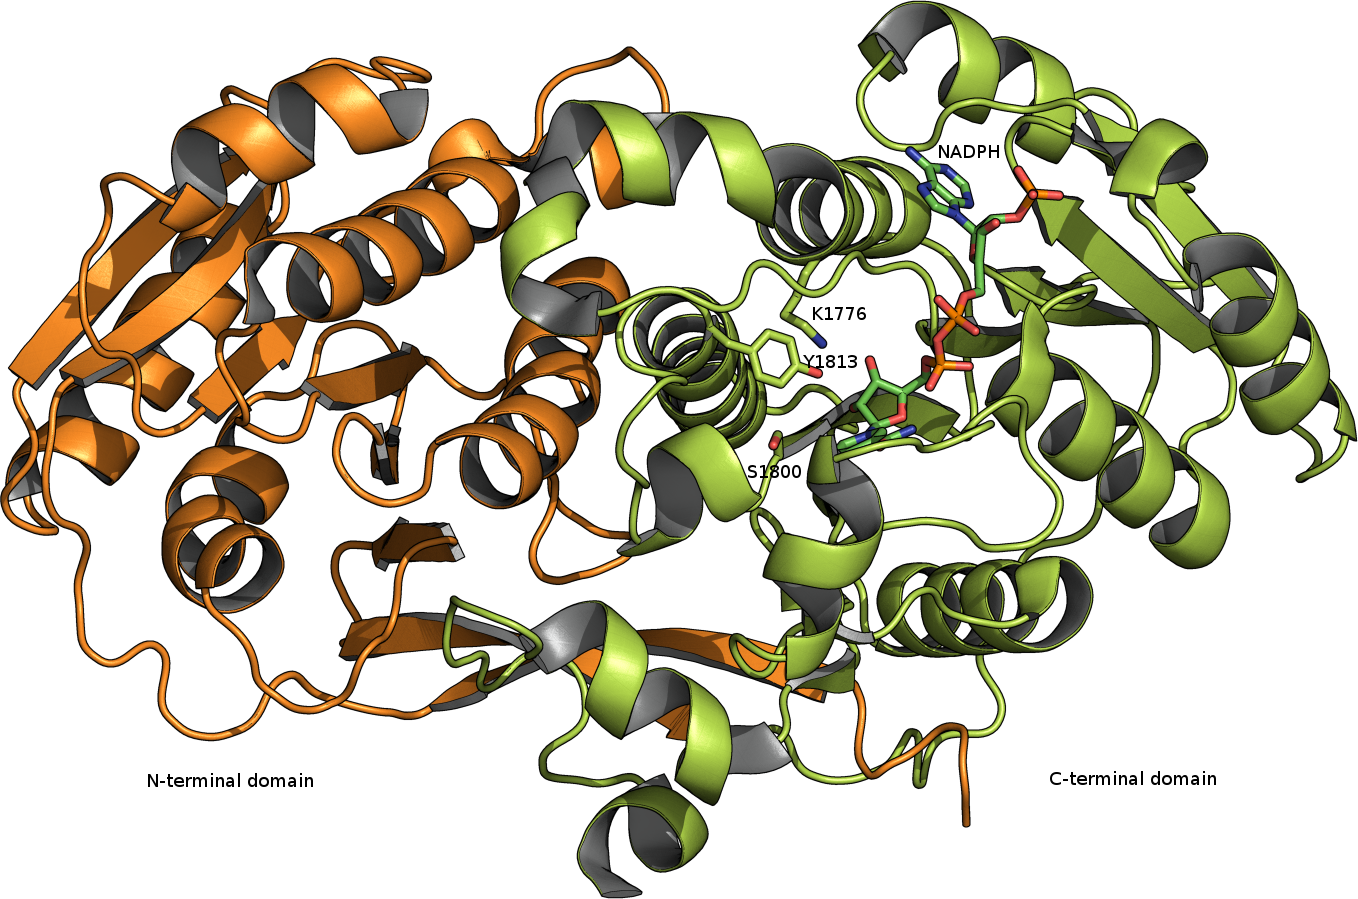
\includegraphics[width=0.8\textwidth, keepaspectratio=true]{graphics/KR.png}}
			\caption[Cartoon representation of a keto reductases domain]{Cartoon representation of a keto reductases domain from the first module of DEBS biosynthesis pathway (PDB ID 2Fr0). The N-terminal structural domain (orange) and the C-terminal catalytic domain (lime) are highlighted along with the catalytic triad Y1813, S1800 and K1776 drawn as sticks. The bound NADPH molecule is shown as sticks \parencite{Keatinge-Clay2006}.}
			\label{fig:KR}
			\end{sidewaysfigure}
			
			Ketoreductases can be classified into three types, type A which is responsible for L-$ \beta $-hydroxyl group, type B for D-$ \beta $-hydroxyl group and type C which are incapable of \bet-keto reduction. Type A and B can be further sub classified as 0, and 1 and 2 depending upon whether they reduce an un-$\alpha$-substituted substrate or an $\alpha$-substituted substrate. A0 and B0 will be type A and B which cater an un-$\alpha$-substituted substrate whereas A1, B1 accepts D-$\alpha$-substituted substrates and A2, B2 accepts L-$\alpha$-substituted substrates  (i.e. [LD]-$ \alpha $-alkyl-[LD]-$ \beta $-hydroxyl). The type C KRs can also be sub classified as C1, which are non functional, and C2, which do not perform \bet-keto reduction but are capable of epimerase activity for the $\alpha$-substituted substrates \parencite{Keatinge-Clay2007}. These classifications were made on the basis of the conserved motifs found through sequence analysis and subsequent mutagenesis and domain swap experiments \parencite{Caffrey2003, Zheng2011}. 
			
			Ketoreductases belong to the superfamily of short chain dehydrogenases/reductases (SDR) and their structures is made up of two Rossmann like fold domains for $\approx$480 residues. The N-terminal structural domain (KR$ _{s} $) does not catalyse the reduction but is thought to be important for providing correct orientation to the C-terminal catalytic domain (KR$_{ c} $). The junction of the  (KR$ _{s} $) and (KR$_{ c} $) is marked by the N-terminal $ \beta $ ($ \beta1 $) strand of (KR$ _{s} $) which is also thought to mark the boundary of the KR, forms a continuous $ \beta $ sheet with the C-terminal $ \beta $ ($ \beta7 $) strand leading to the (KR$_{ c} $) domain. Similar to the SDRs, KRs in modular polyketide synthases were hypothesized to involve the conserved catalytic triad of tyrosine, serine and lysine to carry out \bet-keto reduction \parencite{Keatinge-Clay2006, Zheng2011}. Homology modelling of KR6 from the DEBS3 and subsequent mutagenesis study on the catalytic residues proved the importance of these residues in the \bet-keto processing. \textcite{Reid2003} found that in the complete DEBS system a KR6 Y2699F mutation completely abolishes the pathway whereas KR6 K2664Q and KR6 S2686A significantly reduce polyketide production. However, in a truncated DEBS Module6+TE system all the three KR6 mutations completely abolish the triketide production. Figure \ref{fig:KR} shows the equivalent positions of the catalytic residues in the KR crystal structure from the first module of the DEBS biosynthesis pathway. In the proposed reaction mechanism for the PKS KR, similar to SDRs the catalytic tyrosine was responsible for donating the proton to the carbonyl oxygen of the substrate. Serine provided stability to the ligand through hydrogen bonds and lysine was hypothesized to lower the P$ _{k} $a of the catalytic tyrosine to assist proton transfer. All the KRs from the DEBS system were also shown to utilize pro-S hydride of NADPH. For the L and D configuration of the resultant \bet-hydroxyl group it was proposed that keeping the position of the catalytic residues and the bound cofactor (NADPH) fixed there could be two ways in which the substrate presents the \bet-carbonyl to the active sites (Figure \ref{fig:KRreact}). 

			\setlength\fboxsep{5pt}
			\setlength\fboxrule{1.5pt}
			\begin{figure} []
			\centering
			\fbox{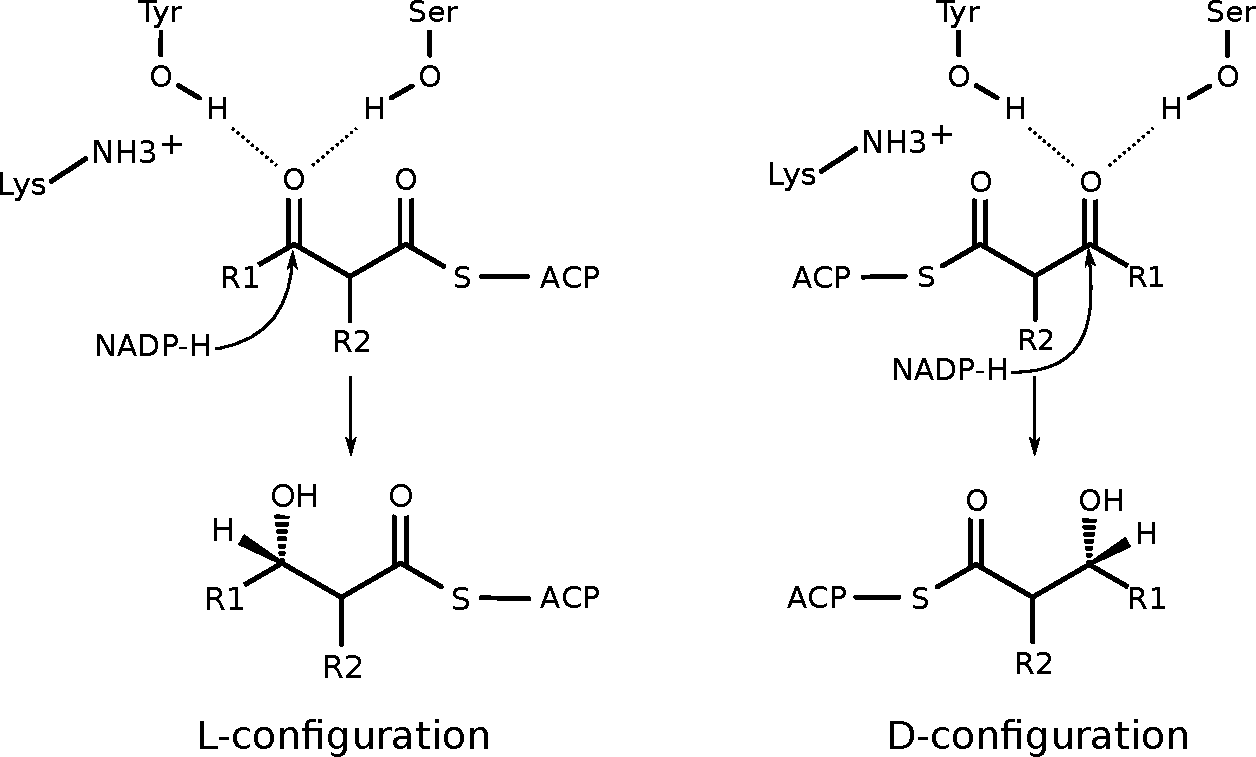
\includegraphics[width=0.95\textwidth, resolution=600, keepaspectratio=true]{graphics/KRreact.pdf}}
			\caption[Proposed reaction mechanism for \bet-keto reduction]{Proposed reaction mechanism for \bet-keto reduction. Figure adapted from \parencite{Reid2003}.}
			\label{fig:KRreact}
			\end{figure}
						
			

			\subsubsection{Dehydratases (DH)}
			\label{sec:DH} 
			DH domains catalyse the reversible dehydration of \bet-hydroxy acyl-ACP to $\alpha,\beta$-unsaturated acyl-ACPs in \textit{cis} or \textit{trans} configuration. The dehydratase domains in the bacterial FAS forms a dimer in a structural fold called a \textquotedblleft hot dog\textquotedblright (Figure \ref{fig:DH}). This hot dog fold comprises a central helix enveloped by the seven \bet-strands. In this hot dog dimeric structure there were two active sites formed at the interface in which an active site dyad histidine is contributed from one subunit and an aspartate from the other subunit. On the contrary the DHs in both the mammalian FAS and dimeric PKS (for example curacin DHs)  are formed of dimers of double hotdog folds in which the histidine and aspartate are provided by the N and C-terminal hotdog respectively (Figure \ref{fig:DH}). The orientation of the dimers in the mammalian FAS and dimeric PKS were different with respect to each other \parencite{Akey2010}. In the proposed reaction mechanism the catalytic histidine which acts as a general base helps in the removal of the proton from the $\alpha $ position and aspartate helps in the removal of \bet-hydroxyl (Figure \ref{fig:DHreact}). The stereochemistry of the dehydrated product is thought to be dependent on the configuration of the \bet-hydroxyl group \parencite{Keatinge-Clay2006, Maier2008, Akey2010}. 
			
			\setlength\fboxsep{5pt}
 			\setlength\fboxrule{1.5pt}
			\begin{figure} []
			\centering
			\fbox{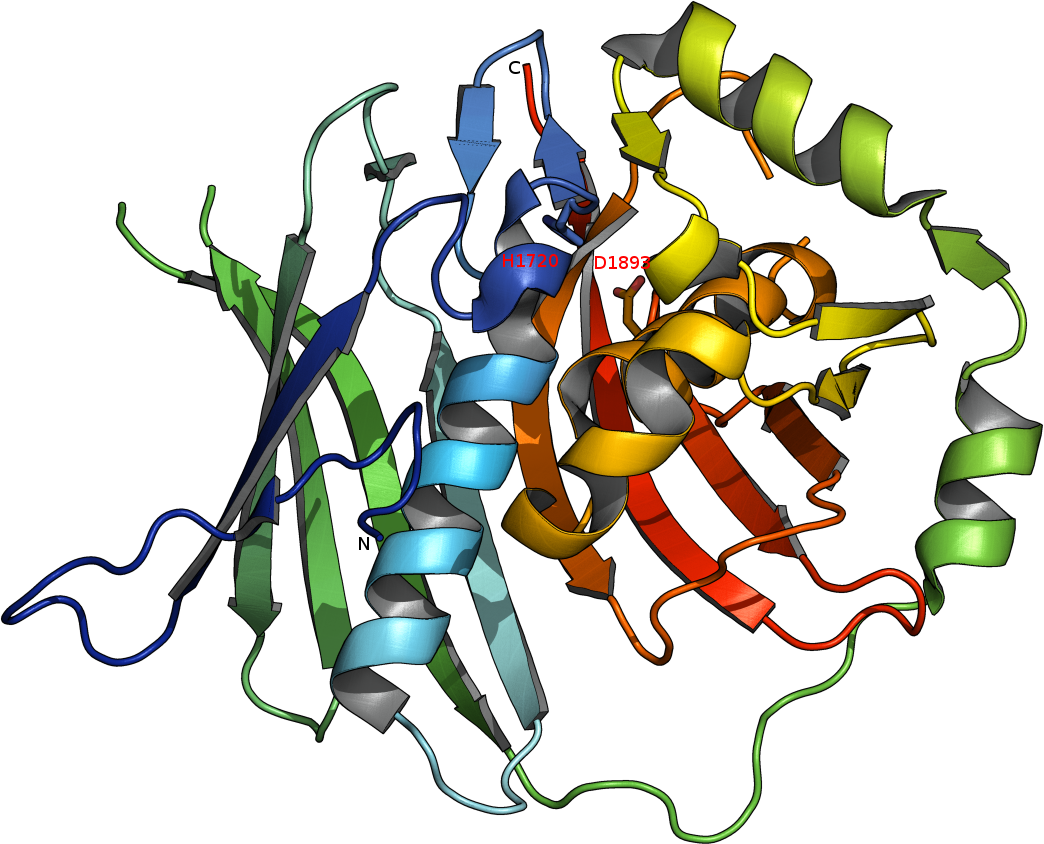
\includegraphics[width=0.95\textwidth, keepaspectratio=true]{graphics/dh.png}}
			\caption[Cartoon representation of the dehydratases domain from curacin biosynthesis pathway]{Cartoon representation of the dehydratases monomer domain (CurF PDB ID 3KG6 chain A) from curacin biosynthesis pathway. The double hot dog structure is coloured in rainbow colours with blue at the N-terminal and red at the C-terminal. The catalytic diad H1720 and D1893 are drawn in sticks and labelled \parencite{Akey2010}.  }
			\label{fig:DH}
			\end{figure}
			
			\setlength\fboxsep{5pt}
 			\setlength\fboxrule{1.5pt}
			\begin{figure} []
			\centering
			\fbox{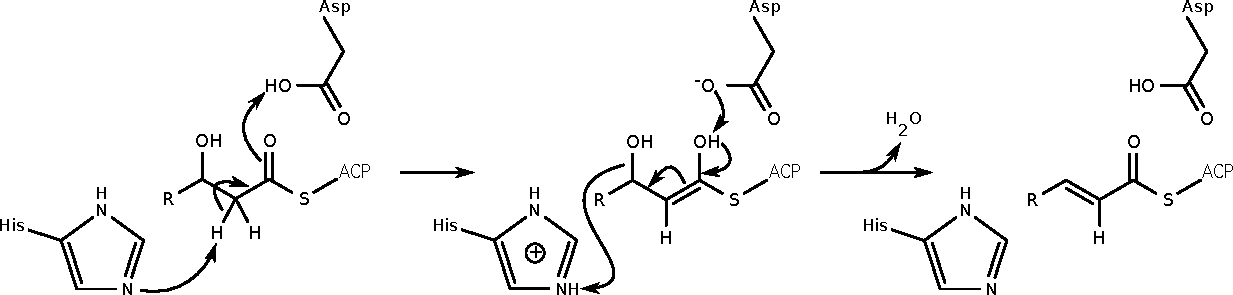
\includegraphics[width=0.95\textwidth, resolution=600, keepaspectratio=true]{graphics/DHreact.pdf}}
			\caption[Proposed reaction mechanism for \bet-hydroxy dehydration]{Proposed reaction mechanism for \bet-hydroxy dehydration.}
			\label{fig:DHreact}
			\end{figure}
			
			\subsubsection{Enoyl reductases (ER)}
			\label{sec:ER}
			The enoyl reductases (ER) in the PKS systems belong to the superfamily of MDR (medium chain dehydrogenase reductases) proteins and are responsible for the reduction of the enoyl-ACP to a fully saturated acyl-ACP on the growing polyketide molecule. These domains usually serve as the last domain in fatty acid and polyketide chain extension and modification cycle before the next round of extension begins. Most of the members of MDR superfamily including ERs exist as homo dimers or tetrameters in FASs and PKSs with the exception of the type I iterative PKS, lovastatin, which contains a free standing monomeric ER (Figure \ref{fig:ER}). 

			\setlength\fboxsep{5pt}
 			\setlength\fboxrule{1.5pt}
			\begin{figure} []
			\centering
			\fbox{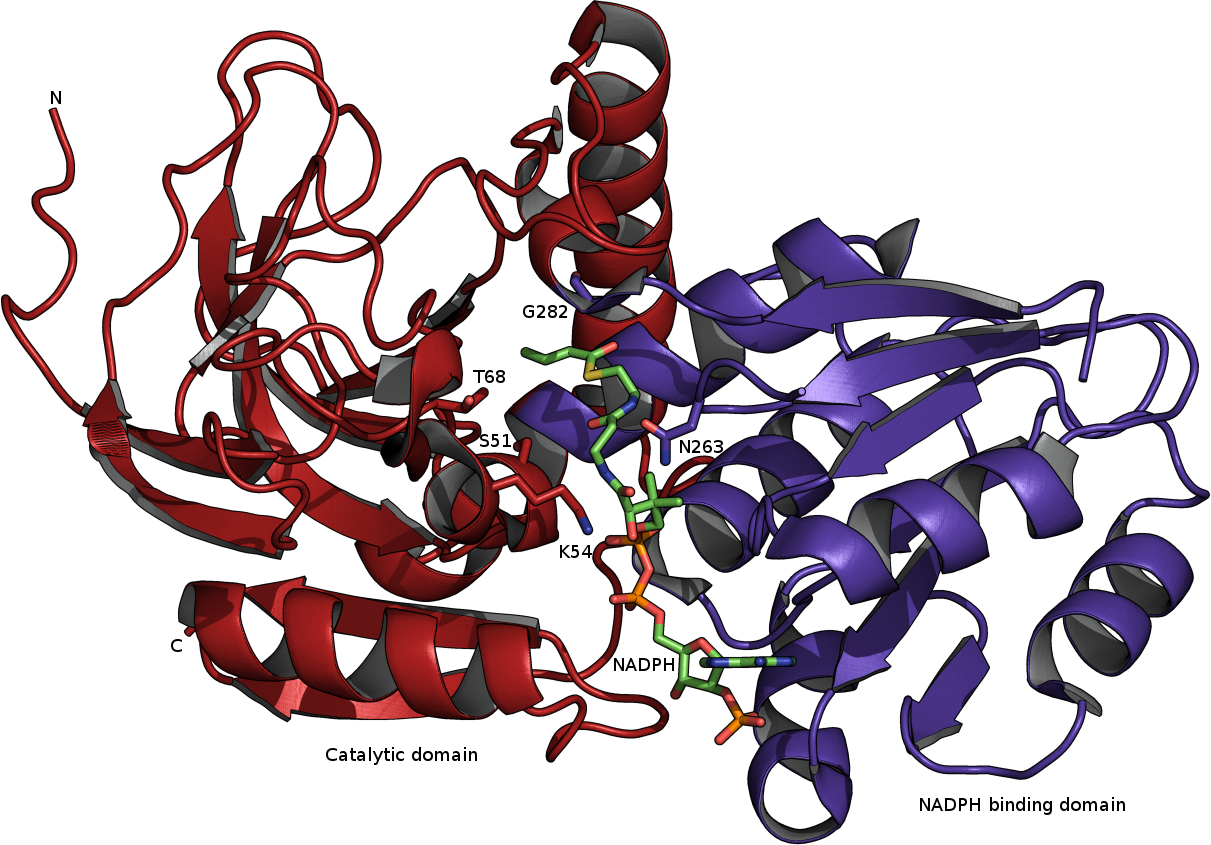
\includegraphics[width=0.95\textwidth, keepaspectratio=true]{graphics/er.png}}
			\caption[Cartoon representation of the enoyl reductase domain from the lovastatin biosynthesis pathway]{Cartoon representation of the enoyl reductase domain from the lovastatin biosynthesis pathway (LovC PDB ID 3B6Z). The catalytic domain (fire brick red) and the NADPH binding domain (purple blue) are separately highlighted. The key active site  resides  S51, K54, T68, N263 and G282 and NADPH are drawn as sticks and labelled \parencite{Ames2012}. }
			\label{fig:ER}
			\end{figure}
						
			The lovastatin ER lovC is composed of two domains the catalytic domain and the cofactor binding domain (Rossmann fold), these structural domains were also found in the other members of the MDR superfamily. The crystal structure solved by \textcite{Ames2012} and subsequent mutagenesis studies have shown key residues which are responsible for LovC catalysis. Figure \ref{fig:ER} highlights the active site residues S51, K54, T68, N263 and G282 in the LovC crystal structure responsible for the oxyanion hole formation and catalysis. In the proposed reaction mechanism (Figure \ref{fig:ERreact} ) K54 and G282 (backbone amide) participate in the oxyanion hole formation to stabilize the enolate oxide formed due to the pro-R hydride transfer from an NADPH. In the next step the enolate oxide accepts a proton most likely from a water molecule and produces a fully saturated $\alpha,\beta$-acyl-ACP. However, the ER in the type I fungal FAS is an exception to this commonly followed reaction mechanism in which the proton is not transferred by an NADPH but instead it utilizes flavin mononucleotide \parencite{Ha2006}. 
			
			The co-factor (NADPH) binding domain  can be characterised by the presence of GXGXXG / AXXXG / A motif and in the DEBS ER4, mutating the NADPH binding motif HAAAGGVGMA to HAAASPVGMA completely abolishes the ER activity. Experiments have shown that ERs have broad substrate specificity and can easily be swapped across different pathways in both FAS and PKS systems \parencite{Khosla1999, Witkowski2004a, Khosla2007}.

			\setlength\fboxsep{5pt}
 			\setlength\fboxrule{1.5pt}
			\begin{figure} []
			\centering
			\fbox{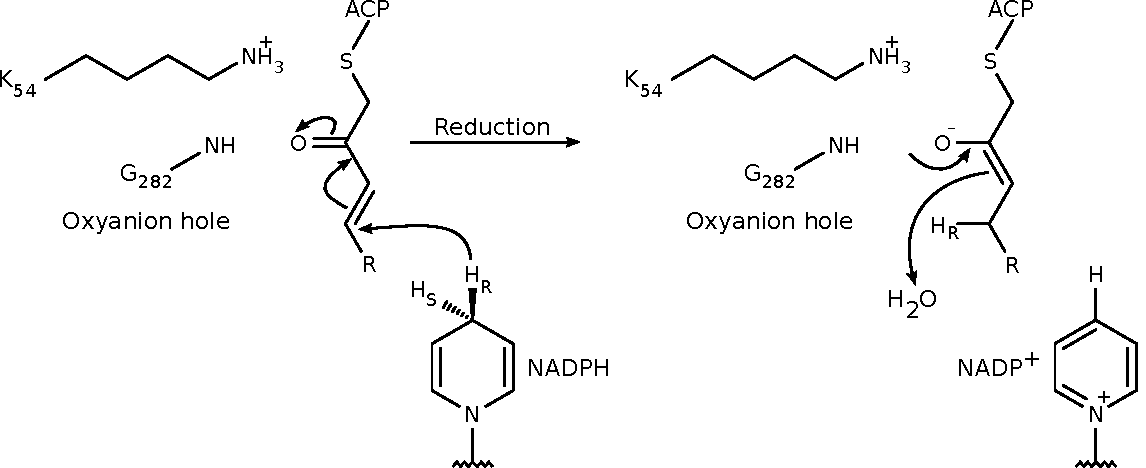
\includegraphics[width=0.95\textwidth, resolution=600, keepaspectratio=true]{graphics/ERreact.pdf}}
			\caption[Proposed reaction mechanism for enoyl reduction]{Proposed reaction mechanism for enoyl reduction in lovastatin biosynthesis pathway (LovC). Figure adapted from \parencite{Ames2012}.}
			\label{fig:ERreact}
			\end{figure}			
						
			\subsubsection{Thioesterases (TE)}
			\label{sec:TE}
			Thioesterases (TE) are the domains responsible for the hydrolytic release and sometimes macro-cyclization  of the polyketide chain attached to an ACP. In modular PKSs, TEs are usually the terminal domains however, experiments from Khosla's group have shown that TE domains are also capable of performing well when attached to a bi modular DEBS1 subunit \parencite{Gokhale1999a}. Thus, TE domains are capable of exhibiting a broad range of substrate tolerance. TE domains have a typical $ \alpha/\beta $ hydrolase fold and a S, H and A catalytic triad, both in the type I modular PKSs and type II fungal iterative PKSs. In the DEBS system the hydrolytic release of the polyketide chain has been proposed as a two step process, in the first step the catalytic S142 initiates a nucleophilic attack on the incoming polyketide intermediate resulting in the transacylation of the acyl chain to the catalytic S142 forming an acyl-enzyme complex. In the second step H259 helps to deprotonate the C-13 hydroxyl on the TE bound polyketide intermediate which results in the release and macro cyclization of the 6-deoxyerythronolide B. In the DEBS TE the 14 membered ring is also supported by seven hydrogen bonds inside the active site, which ensures the correct orientation of the C-13 hydroxyl group close to the Ser-O-acyl linkage  \parencite{Gokhale1999a, Sharma2007, Khosla2007}. Figure \ref{fig:TE} and \ref{fig:TEreact} show the crystal structure of the TE monomer from the DEBS system with the highlighted active site triad and the proposed reaction mechanism respectively \parencite{Tsai2001}. 

			\setlength\fboxsep{5pt}
 			\setlength\fboxrule{1.5pt}
			\begin{figure} []
			\centering
			\fbox{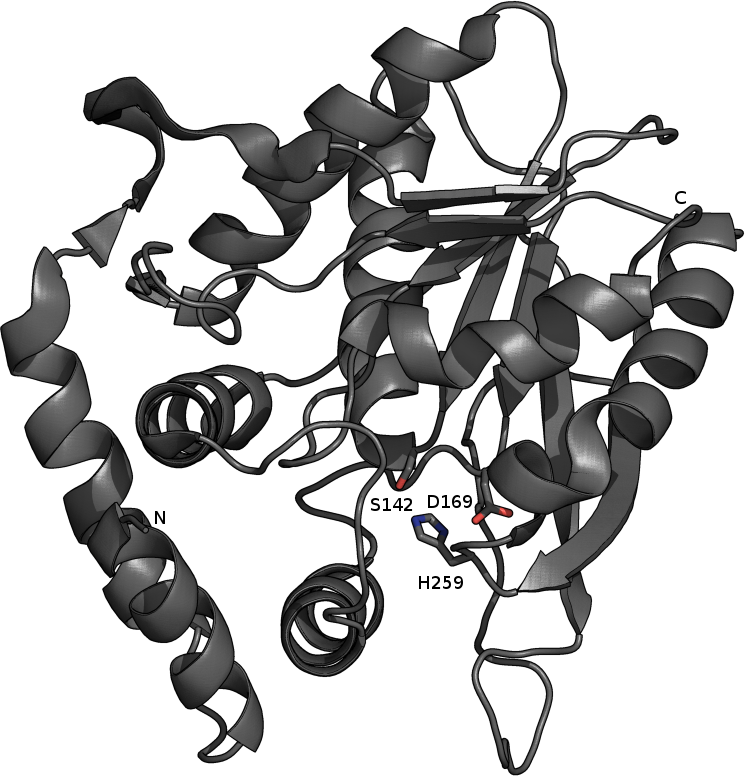
\includegraphics[width=0.7\textwidth, keepaspectratio=true]{graphics/te.png}}
			\caption[Cartoon representation of the thioesterases domain from DEBS biosynthesis pathway]{Cartoon representation of the thioesterases domain monomer from DEBS biosynthesis pathway (PDB ID 1KEZ). The catalytic triad S142, H259 and D169 are drawn as sticks and labelled \parencite{Tsai2001}. }
			\label{fig:TE}
			\end{figure}
			
			\setlength\fboxsep{5pt}
 			\setlength\fboxrule{1.5pt}
			\begin{figure} []
			\centering
			\fbox{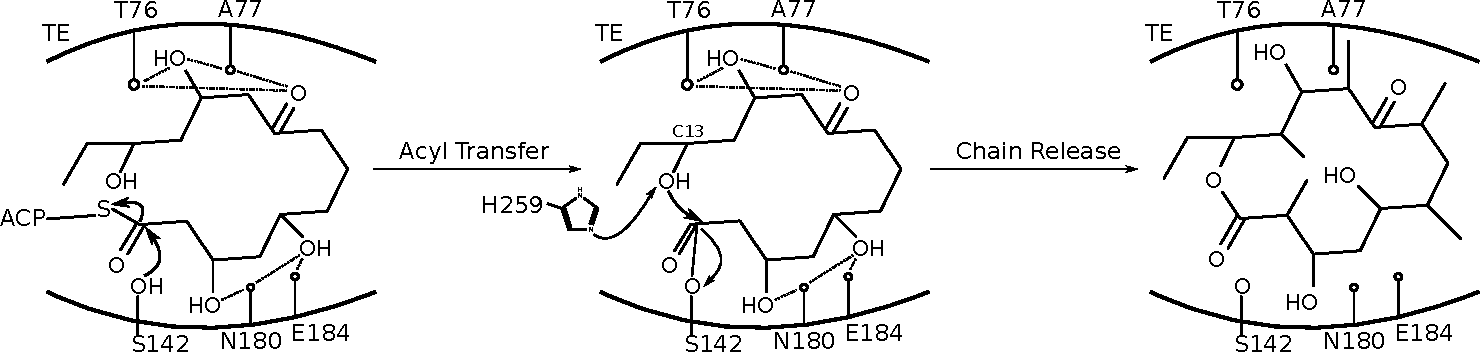
\includegraphics[width=0.95\textwidth, resolution=600, keepaspectratio=true]{graphics/TEreact.pdf}}
			\caption[Proposed reaction mechanism for thioesterase]{Proposed reaction mechanism for thioesterase in DEBS biosynthesis pathway. Hydrogen bonds are drawn as dotted lines. Figure adapted from \parencite{Tsai2001}.}
			\label{fig:TEreact}
			\end{figure}			
\newpage						
		\subsection{Complete modular structures of FAS/PKS}
		\label{sec:PKSstructure}
		The earliest attempts made to experimentally determine the complete modular structure of an FAS  were carried out in the late 1980s using small angle neutron scattering and electron microscopy using samples from chicken, pig and human FAS \parencite{Stoops1987, Kitamoto1988, Brink2002}. Owing to the poor quality of the electron density measured those models were only used to support the feasibility of the previously proposed head-to-head model over the fully extended head-to-tail model. Those models were also not good enough to correctly determine whether the two chains of the FAS were arranged in a back to back manner or were crossed over. 
		
		In the mid 2000s Nenad Ban and his colleagues were able to successfully determine the structure of a complete FAS module from mammalian and fungal species through X-ray crystallography at various resolutions \parencite{Maier2006, Jenni2007, Maier2008}. And later on in 2013 they produced a cryo-EM structure of the Mycobacterial FAS \parencite{Boehringer2013}. Similar to the previous attempts Ban's group also struggled in correctly determining the structure of the highly flexible regions such as the terminal ACP and the TE domains and it was only the yeast FAS in which they could successfully locate the position of the ACP. All the other structures were determined without the ACP and the TE domain.
		
		\subsubsection{Mammalian FAS}
		\label{sec:mFAS}
		The first crystal structure determined by the Ban group was the 4.5 \AA{} resolution mammalian FAS an  $ \alpha_{2}$-homodimeric protein with all the seven FAS domains on each of the two subunits. In spite of being successful in obtaining crystals of the porcine FAS the resolution was not good enough to correctly determine the position of the side chains in the molecule however, the secondary structural elements were clearly detectable. Therefore, they utilized the electron density map to fit the previously determined crystal structures of individual domains from type II FAS to obtain a domain architecture of the mammalian FAS (PDB ID 2CF2) \parencite{Maier2006}. 
		
		The overall shape of the mammalian FAS was like an X, imagining this as a person, the KS homodimers form the lower and DH domain pseudo dimers form the upper portion of the torso of the body, the MAT domains forming the legs attached to the KS, the ER domain homo dimer the head and the KR domains forming the arms (Figure \ref{fig:mammalianFasStructure}). This arrangement of the domains in the quaternary structure was in contrast to the linear arrangement of the domains in the primary structure and has dimensions of 210 \AA{} x 180 \AA{} x 90 \AA{}. The architecture also revealed two main dimerization interfaces, one at the KS and the other at the ER domains covering an area of $\approx$5000 $ \AA{}^{2} $. The KS dimer was found to be similar to bacterial KS I from FabB and was in agreement with cross linking experiments conducted in the mammalian FAS to cross link the N-terminus of a KS domain with the engineered active site cysteine of the other \parencite{Witkowski2004}. The ER domain homodimers form a continuous 12 stranded beta sheet at the interface joining the two nucleotide binding domains, six strands coming from each monomer. Apart from the dimer interfaces between the KS and the ER domains a small portion of the lower end of the DH domains also contribute to the overall dimer formation. The DH domains sit on top of the KS domains with the lower portion of the DH domains making a contact with the upper portion of the KS, domains which forms the waist like region. Linker regions were found in between the KS and the MAT domain and also between the MAT and DH domain. The KR domains are separate single domains hanging out as arms with no contacts between the two which was contrary to observation of tetrameric bacterial KRs \parencite{Maier2006, Boehringer2013}. 
		
		\textcite{Maier2006} made an interesting observation that the X shape of the mammalian FAS is asymmetrical. The conformation in which the X-ray structure was obtained had different sized reaction centres in the KS domain. The distance between the KRs and the MAT domains on the same sides were not similar and they were measured to be 72 \AA{} on one side and 87 \AA{} on the other. It was speculated that this difference in the size of the reaction centres may be caused by the mechanism of substrate binding to the KS and the product release after elongation, mediated by a hinge in the \textquotedblleft waist\textquotedblright \ region. In support of this hypothesis, the bacterial KSs in FabB have shown non symmetrical mode of substrate binding. They also proposed that the KS/MAT linker region might also allow the MAT domains to  move in the \textquotedblleft up and down\textquotedblright \ direction. The proposed cumulative effect of these motions were to accommodate the ACPs close to the enzymatic domains. As the observed length of the phosphopantetheine arm was only long enough for the bound substrate to reach to the centre of the active sites, implies if the ACPs were in close contact with the individual catalytic domains then there should be enough space in the quaternary arrangement of the FAS domains to accommodate the ACP next to the active site entrance of each domain.  This hypothesis also strengthened by work by \textcite{Zhang2003}, which identified the key residues responsible for the interaction between the ACPs and the KR domains in the bacterial type II FAS, thus proving the existence of domain-domain interaction between the ACPs and the FAS catalytic domains.

			\setlength\fboxsep{5pt}
 			\setlength\fboxrule{1.5pt}
			\begin{figure} []
			\centering
			\fbox{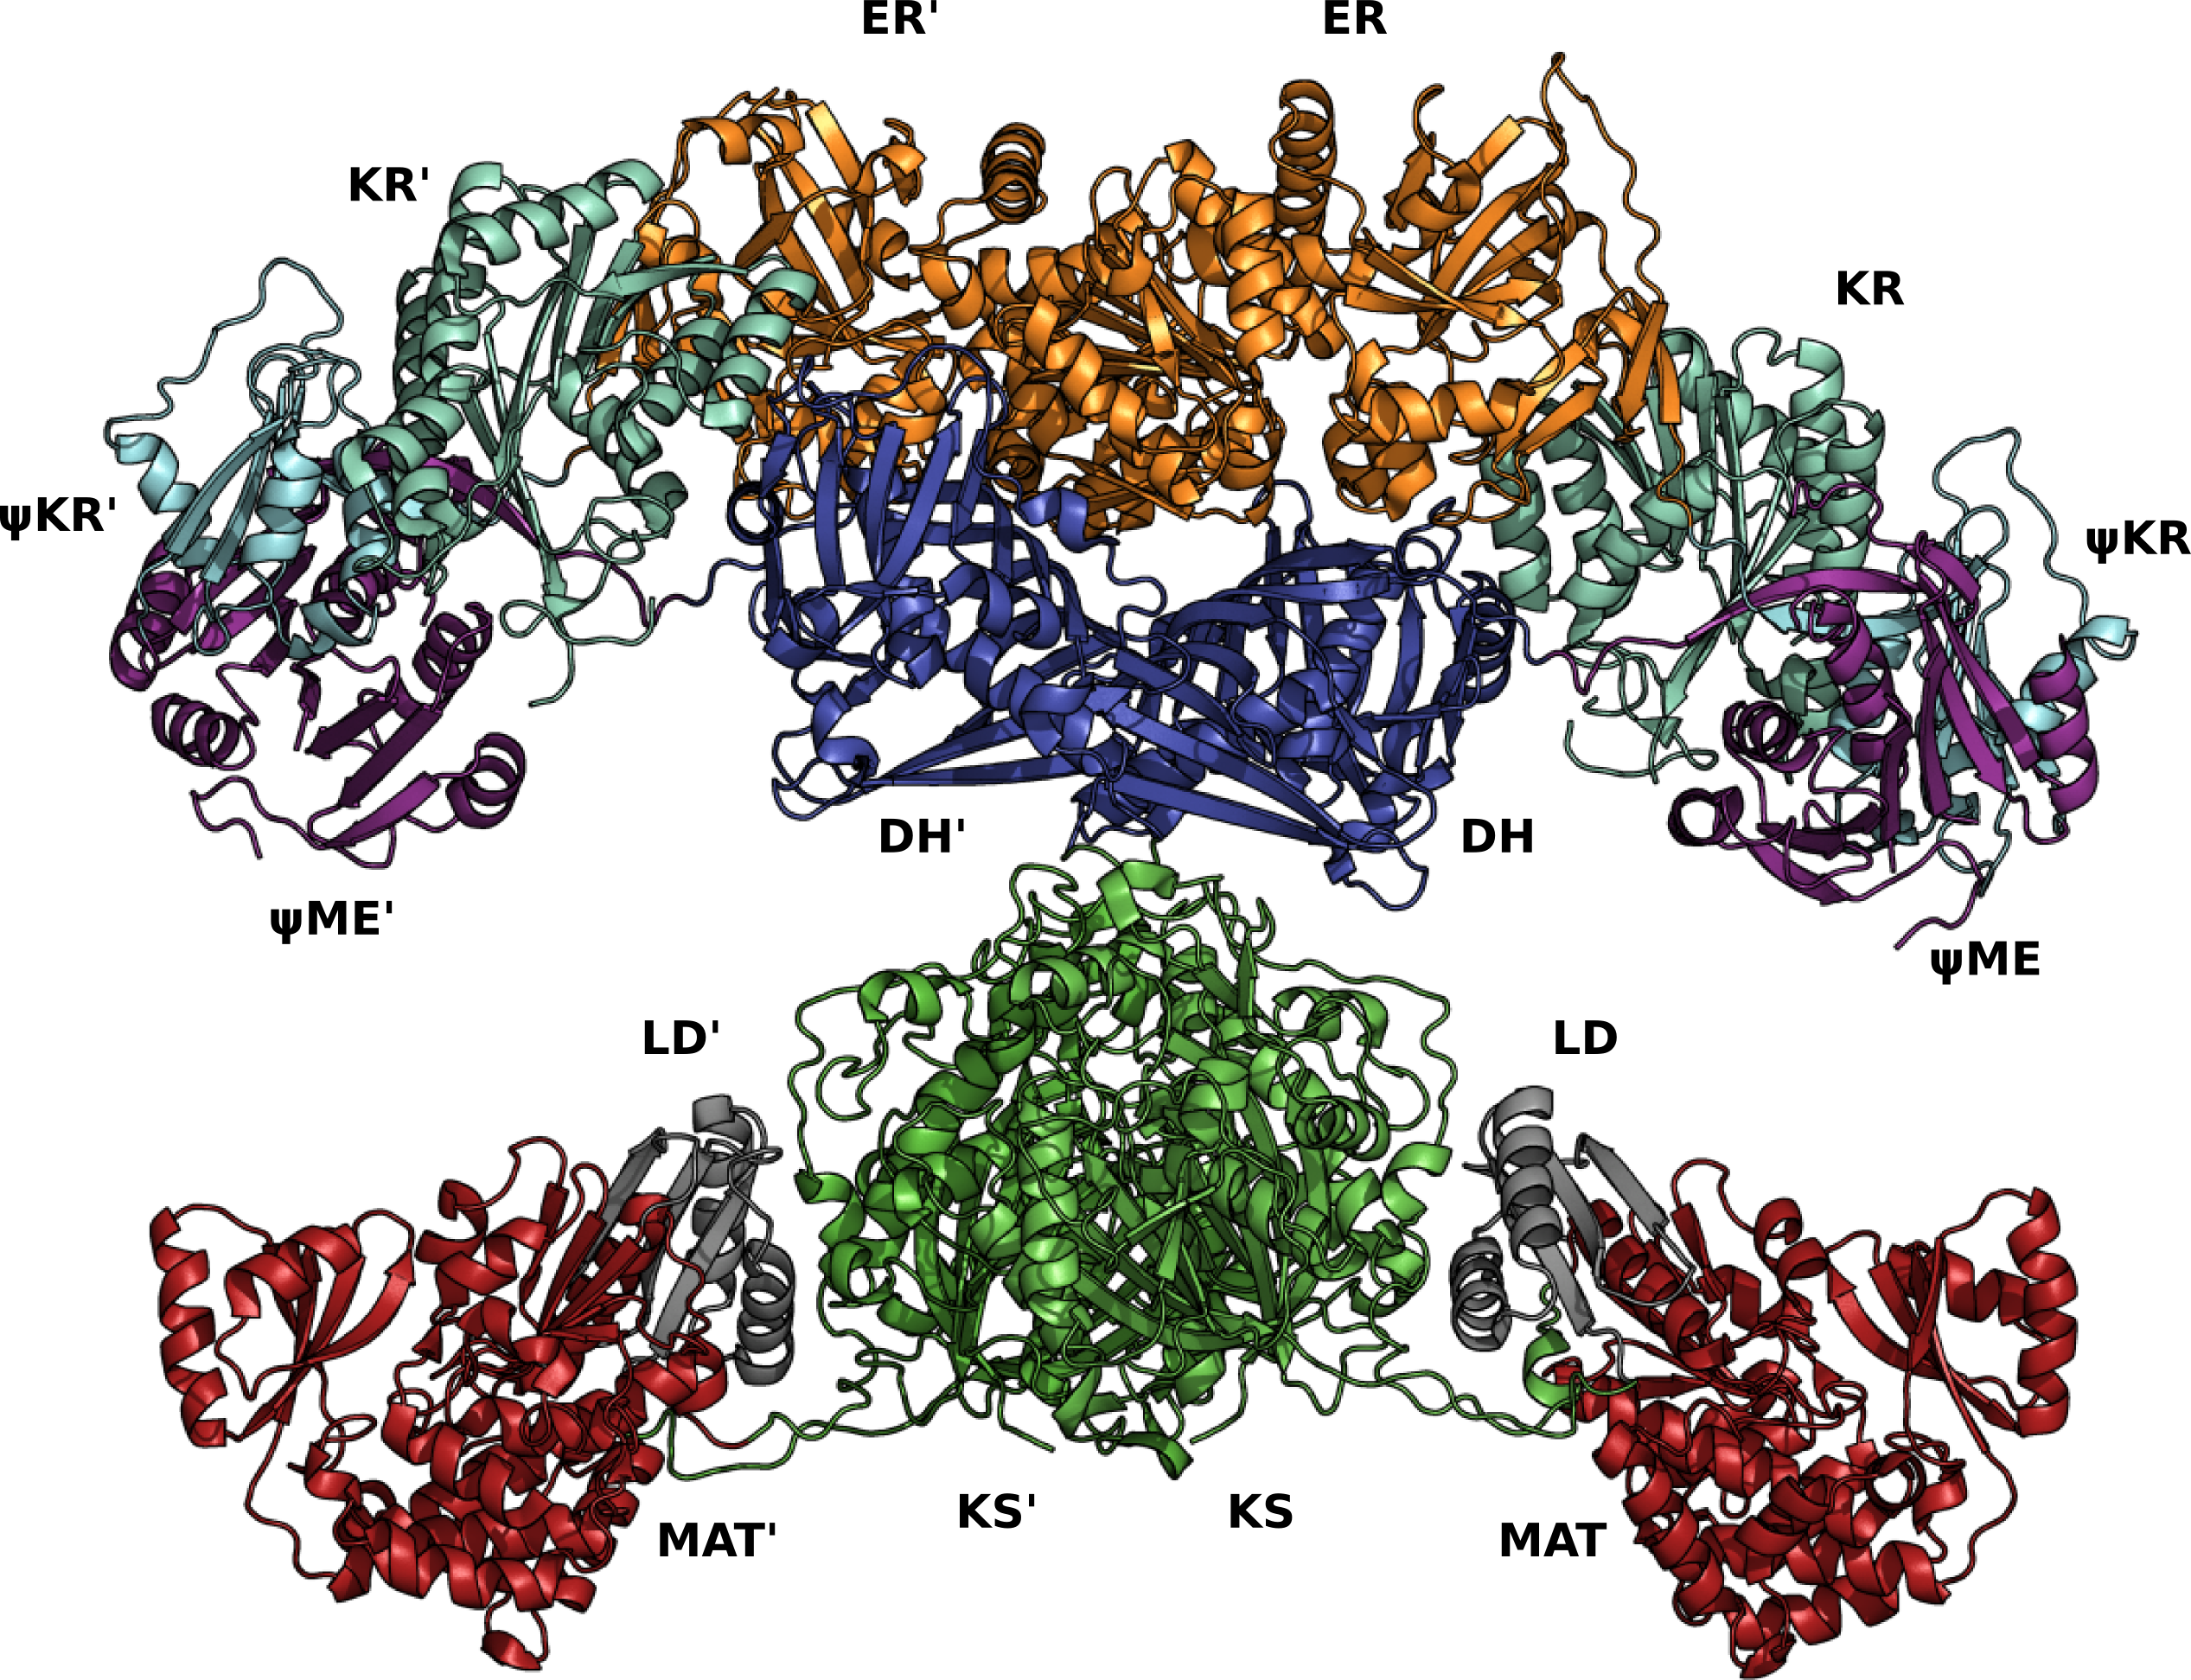
\includegraphics[width=0.95\textwidth, resolution=600, keepaspectratio=true]{graphics/mammalianFasStructure.png}}
			\caption[X-ray structure of the mammalian FAS (PDB ID 2VZ8) rendered as cartoon.]{X-ray structure of the mammalian FAS (PDB ID 2VZ8) rendered as cartoon. The catalytic (KS and MAT) and the modifying domains (KR, DH and ER) are coloured and labelled as indicated. The linker domains (LD) are coloured as grey and the pseudo domains (ME and KR) are labelled with the symbol $ \psi $.}
			\label{fig:mammalianFasStructure}
			\end{figure}			
					
		Following the determination of the mammalian FAS domain architecture based on the 4.5 \AA{} resolution X-ray crystallographic map, Ban's group successfully determined the 3.2 \AA{} resolution crystal structure of FAS in its NADP$ ^{+} $ free and bound states (PDB ID 2VZ8). The resolution for this crystal structure was good enough to correctly determine the side chains along with the secondary structure (Figure \ref{fig:mammalianFasStructure}). However, even in this attempt they couldn't determine the structure for the ACP and the TE domains. The 3.2 \AA{} resolution structure also agreed with the previously observed X shaped domain organization of the mammalian FAS. However, they identified two additional structural domains. One of the additional domains resembled a methyl transferase but is apparently catalytically inactive, and thus referred to as pseudo methyl transferase, and the other domain was similar to a ketoreductase which was thought to provide structural scaffold for the correct orientation of the catalytically active KR. This structure had similar dimerisation interfaces between the KS and the ER domains to those observed in the 4.5 \AA{} resolution model. However, the size measured was according to the electron density observed for the mammalian FAS side chains rather than the fit from the type II FAS discrete domains. The overall contact area in the dimerisation interface of the 3.2 \AA{} was measured to be 5400 $ \AA{}^{2} $ which included 150 amino acids with the contributions of $\approx$2600 and 1600 $ \AA{}^{2} $ from KS and ER domains respectively. The two DH domains also contributed 800 $ \AA{}^{2} $ to the dimerization interface along with the linker region between MAT, DH and the KS domains. This crystal structure also revealed the linker regions between the KS and the MAT domains, consisting of two helices and three \bet-strands forming an anti parallel \bet-sheet. This linker, which was thought to prevent any direct linkage between the KS and MAT domains, was also observed in the KS-AT crystal structure in the type I modular DEBS PKS determined at the same time by Khosla's group \parencite{Tang2006, Tang2007}. On the basis of the sequence context this region was also speculated to be present in the trans AT systems and a very recent crystal structure of the KS homodimers from a trans AT system showed the presence of a similar linker region attached to the C-terminal of the KS domains \parencite{Gay2014}. The precise role of this linker region is still unknown however experiments from Khosla's group have shown that they might be necessary for the ACP docking during the elongation and acyl-transfer stages \parencite{Kapur2010}. 
		
		\subsubsection{Fungal FAS}
		\label{sec:fFAS}
		In 2007 Ban group solved the crystal structure of 2.6 mDa $ \alpha_{6}\beta_{6} $ -dodecameric fungal FAS from \textit{Thermomyces lanuginosus} (PDB ID 4V58)  and that of \textit{Saccharomyces cerevisiae} (PDB ID 2UV8), both at 3.1 \AA{} resolution \parencite{Jenni2007}. The structure determined from \textit{S. cerevisiae} also revealed the position of the ACP attached to the KS active site. Although both the mammalian and fungal FAS are type I FAS where the domains are covalently attached in a single polypeptide their quaternary structures are very different from each other. The fungal FAS structure comprised of a central wheel sandwiched between two dome like structures (Figure \ref{fig:fungalFasStructure}) providing two distinct reaction centres with five entrances through the walls and top of the domes. The two reaction centres were connected by six passages through the central wheel. The central wheel was composed of 6 $ \alpha $ subunits  whereas the domes were composed of 3 $ \beta $ subunits each. One $ \alpha $ and one $ \beta $ subunit join to form a single non-redundant FAS unit. Thus in a fungal FAS complex there are six functional units of FAS formed by 12 polypeptide chains. The $ \alpha $ chains consists of KS and the KR domains and the $\beta$ chains consist of AT, MPT (malonyl/palmitoyl transferase) \nomenclature{MPT}{Malonyl/palmitoyl transferase}, DH and ER domains with numerous inter-chain contacts between the domains. All the active sites were found to point towards the inner side of the catalytic centres in the two domes. The fungal FAS also had phosphopantetheinyl transferase (PPT) domains attached to the C-terminal hanging outside the reaction centres. PPT are responsible for attaching the phosphopantetheine arm to the ACP. 
		
			\setlength\fboxsep{5pt}
 			\setlength\fboxrule{1.5pt}
			\begin{figure} []
			\centering
			\fbox{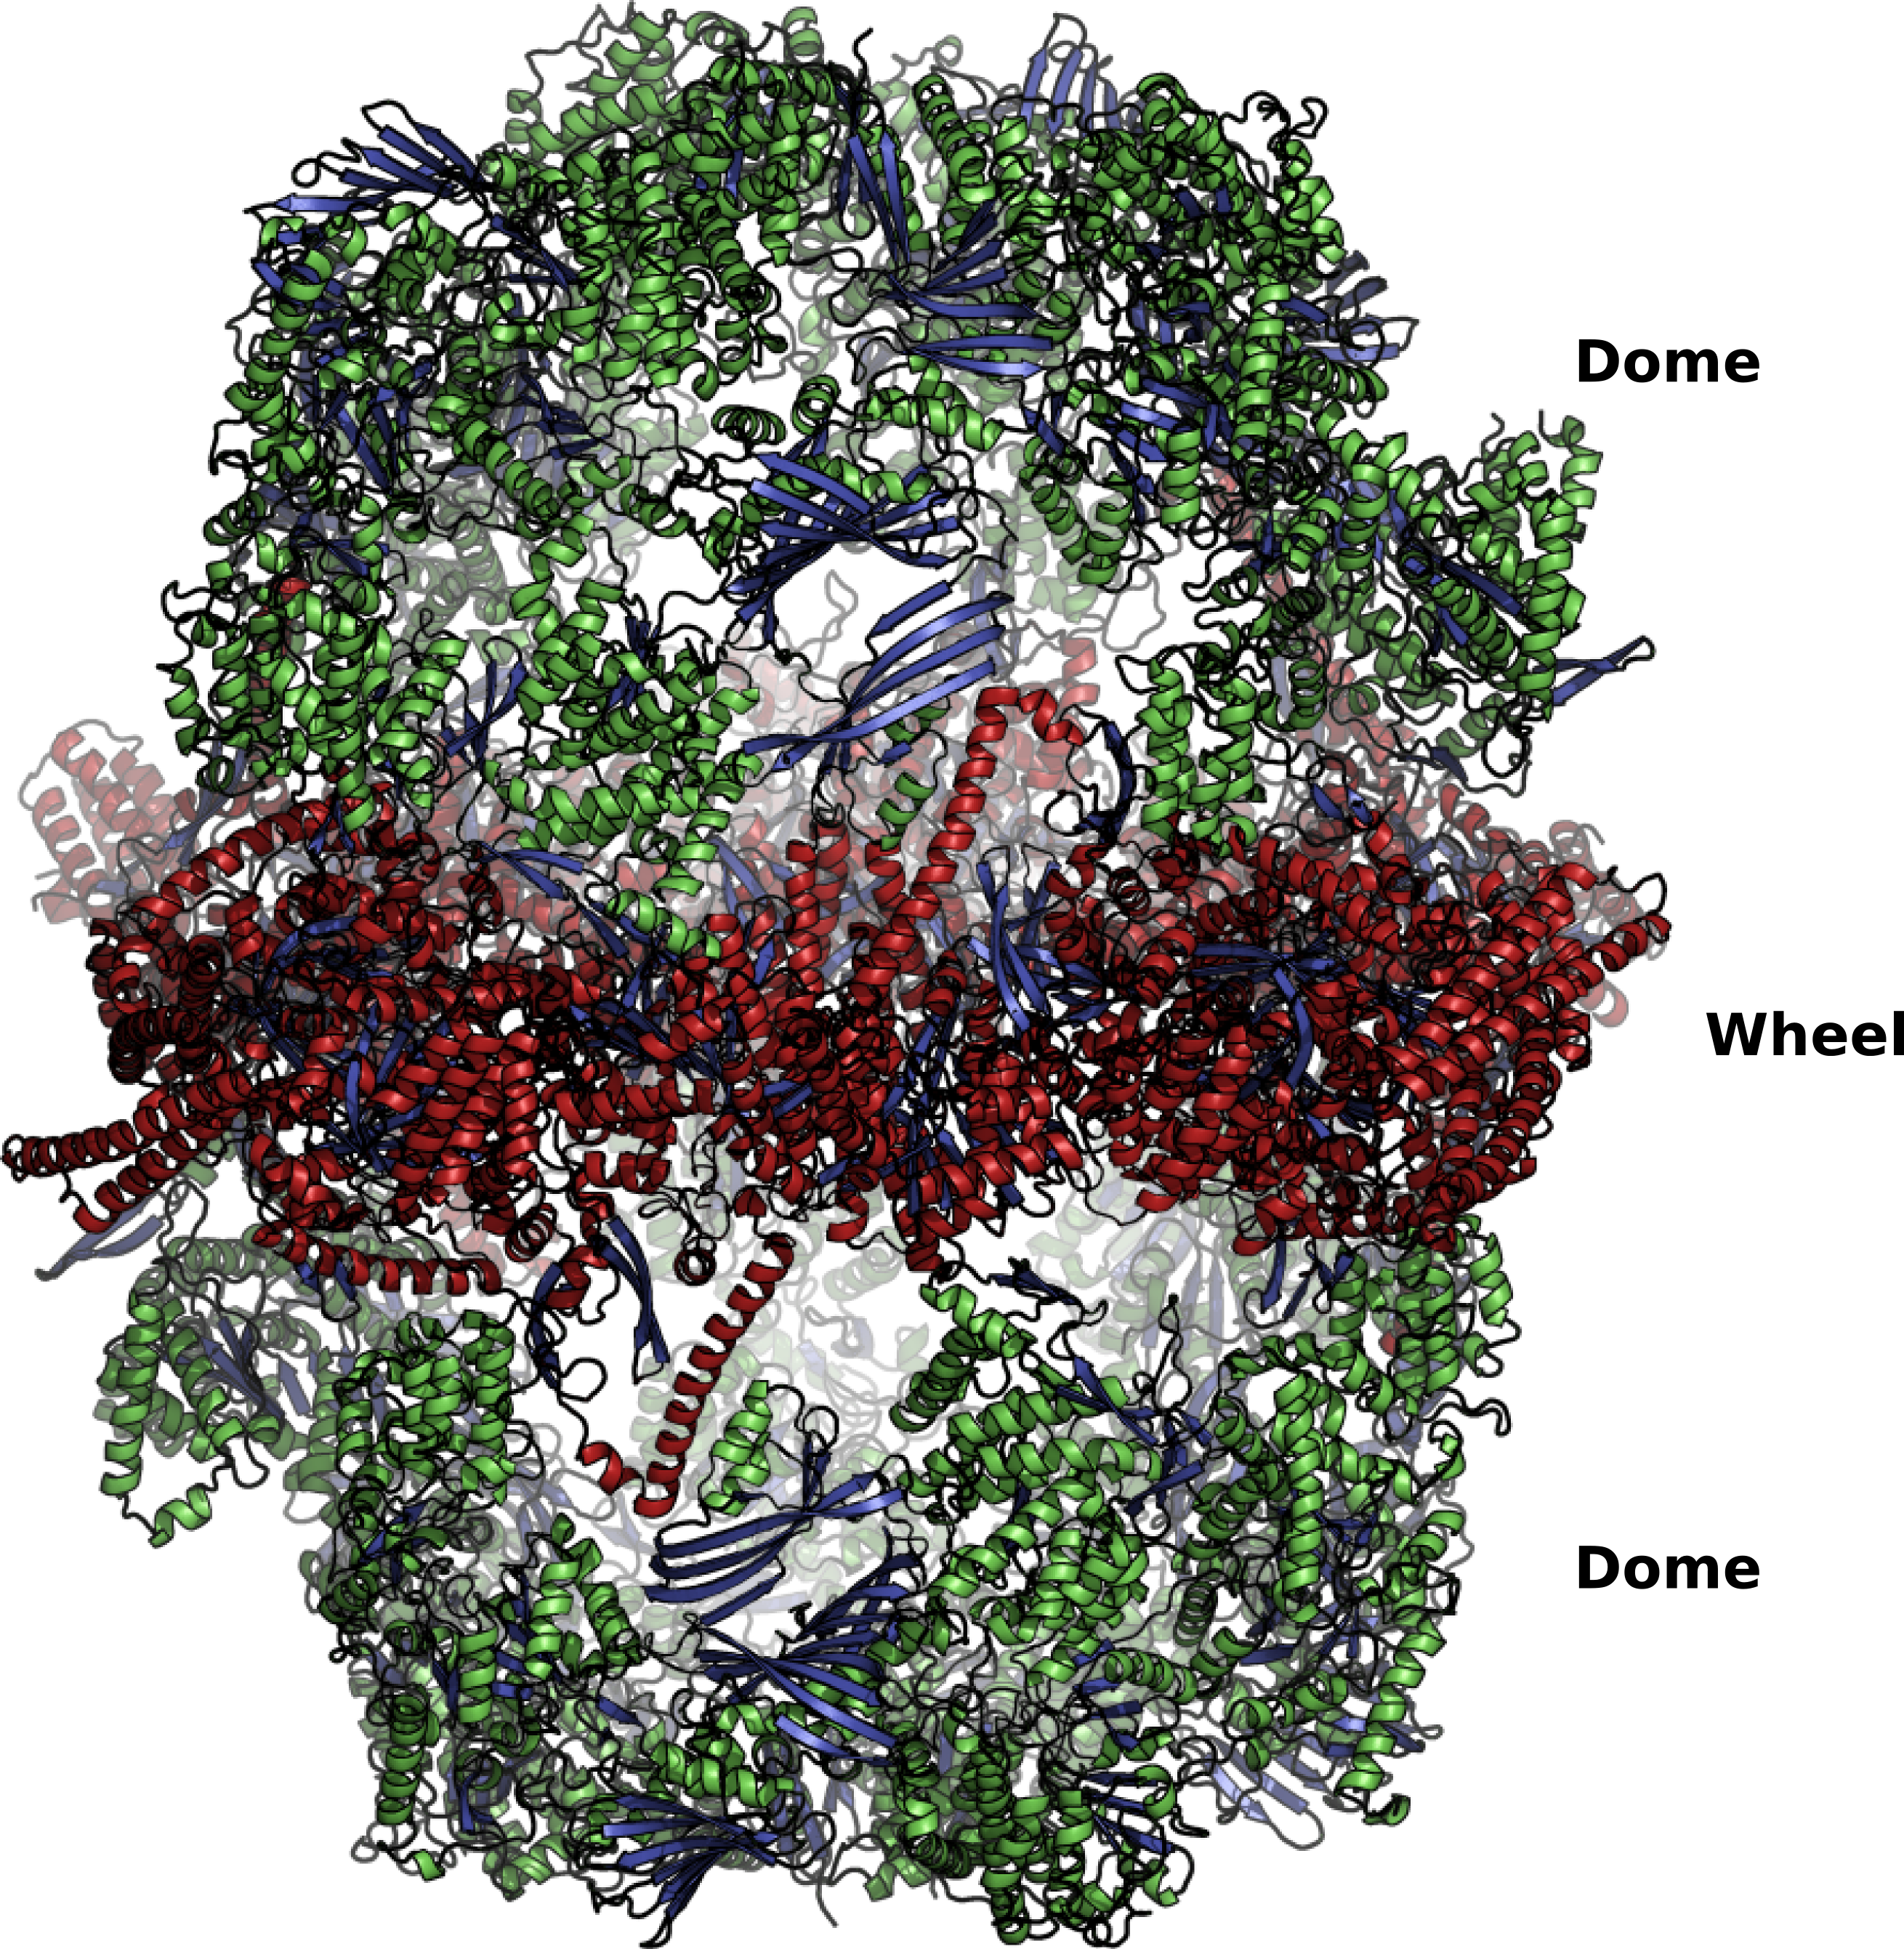
\includegraphics[width=0.95\textwidth, resolution=600, keepaspectratio=true]{graphics/fungalFasStructure.png}}
			\caption[X-ray structure of the fungal FAS (PDB ID 4V58) rendered as cartoon.]{X-ray structure of the fungal FAS (PDB ID 4V58) rendered as cartoon. Helices in the domes and the middle wheel are coloured in green and red respectively. Beta sheets are coloured in blue.}
			\label{fig:fungalFasStructure}
			\end{figure}			
		
		The all helical acyl carrier proteins in the fungal FAS were twice the size of their bacterial counterpart  with the first four helices overlapping very well with their homologues. The catalytic Serine was found to be on a loop between helices 7 and 8 whereas helix 8 was considered to be the recognition helix when making a contact with the KS. There were three ACPs each in both the reaction centres and these are doubly tethered, to the reaction centre wall at the N-terminus and to the central wheel at the C-terminus. The AT and the MPT domains had similar folds and were thought to be involved in charging ACPs with the acetyl or malonyl, and palmitoyl moieties respectively. The fungal FAS KS domains exhibit broad substrate specificity as compared to their bacterial homologues. A single FAS KS is capable of iteratively catalyse fatty acid chain elongation from $ C_{2} $ to $ C_{16} $ whereas three different KS domains are required in the bacterial FAS. All the KS domains were found to be tightly embedded in the central wheel of the fungal FAS with the active sites pointing towards opposite reaction centres. The ketoreductases found in fungal FAS followed the classical Rossmann fold however they were dimeric as compared to the monomeric mammalian and tetrameteric bacterial KRs. The DH domains in the fungal FAS formed a triple hot dog fold as compared to the mammalian double hot dog fold. The ER domains in the fungal FAS were also different from their mammalian and bacterial counterparts since the fungal ER utilizes flavin mononucleotide (FMN) \nomenclature{FMN}{Flavin mononucleotide} instead of an NADPH and forms a TIM barrel as opposed to Rossmann fold \parencite{Jenni2007, Leibundgut2007}.
		
		\subsubsection{Bacterial type I FAS}
		\label{sec:bFAS}
		In the year 2013 Ban's group published the cryo-EM reconstruction of a Mycobacterial FAS structure at 7.5 \AA{} resolution from the \textit{Mycobacterium smegmatis} species (PDB ID 4V8L, \textcite{Boehringer2013}). The Mycobacterial FAS showed a barrel shaped domain architecture similar to the fungal FAS (Figure \ref{fig:mycoFasStructure}). However, the structure was more compact with wider openings for the external entrance into the structures. \textcite{Boehringer2013} used the yeast FAS crystal structure to fit the Mycobacterial EM density map. The 7.5 \AA{} resolution was good enough to detect the individual helices however, the $ \beta $ strands were not clearly visible. Although the flattened shape of the $\beta$ sheets were detectable. 
		
			\setlength\fboxsep{5pt}
 			\setlength\fboxrule{1.5pt}
			\begin{figure} []
			\centering
			\fbox{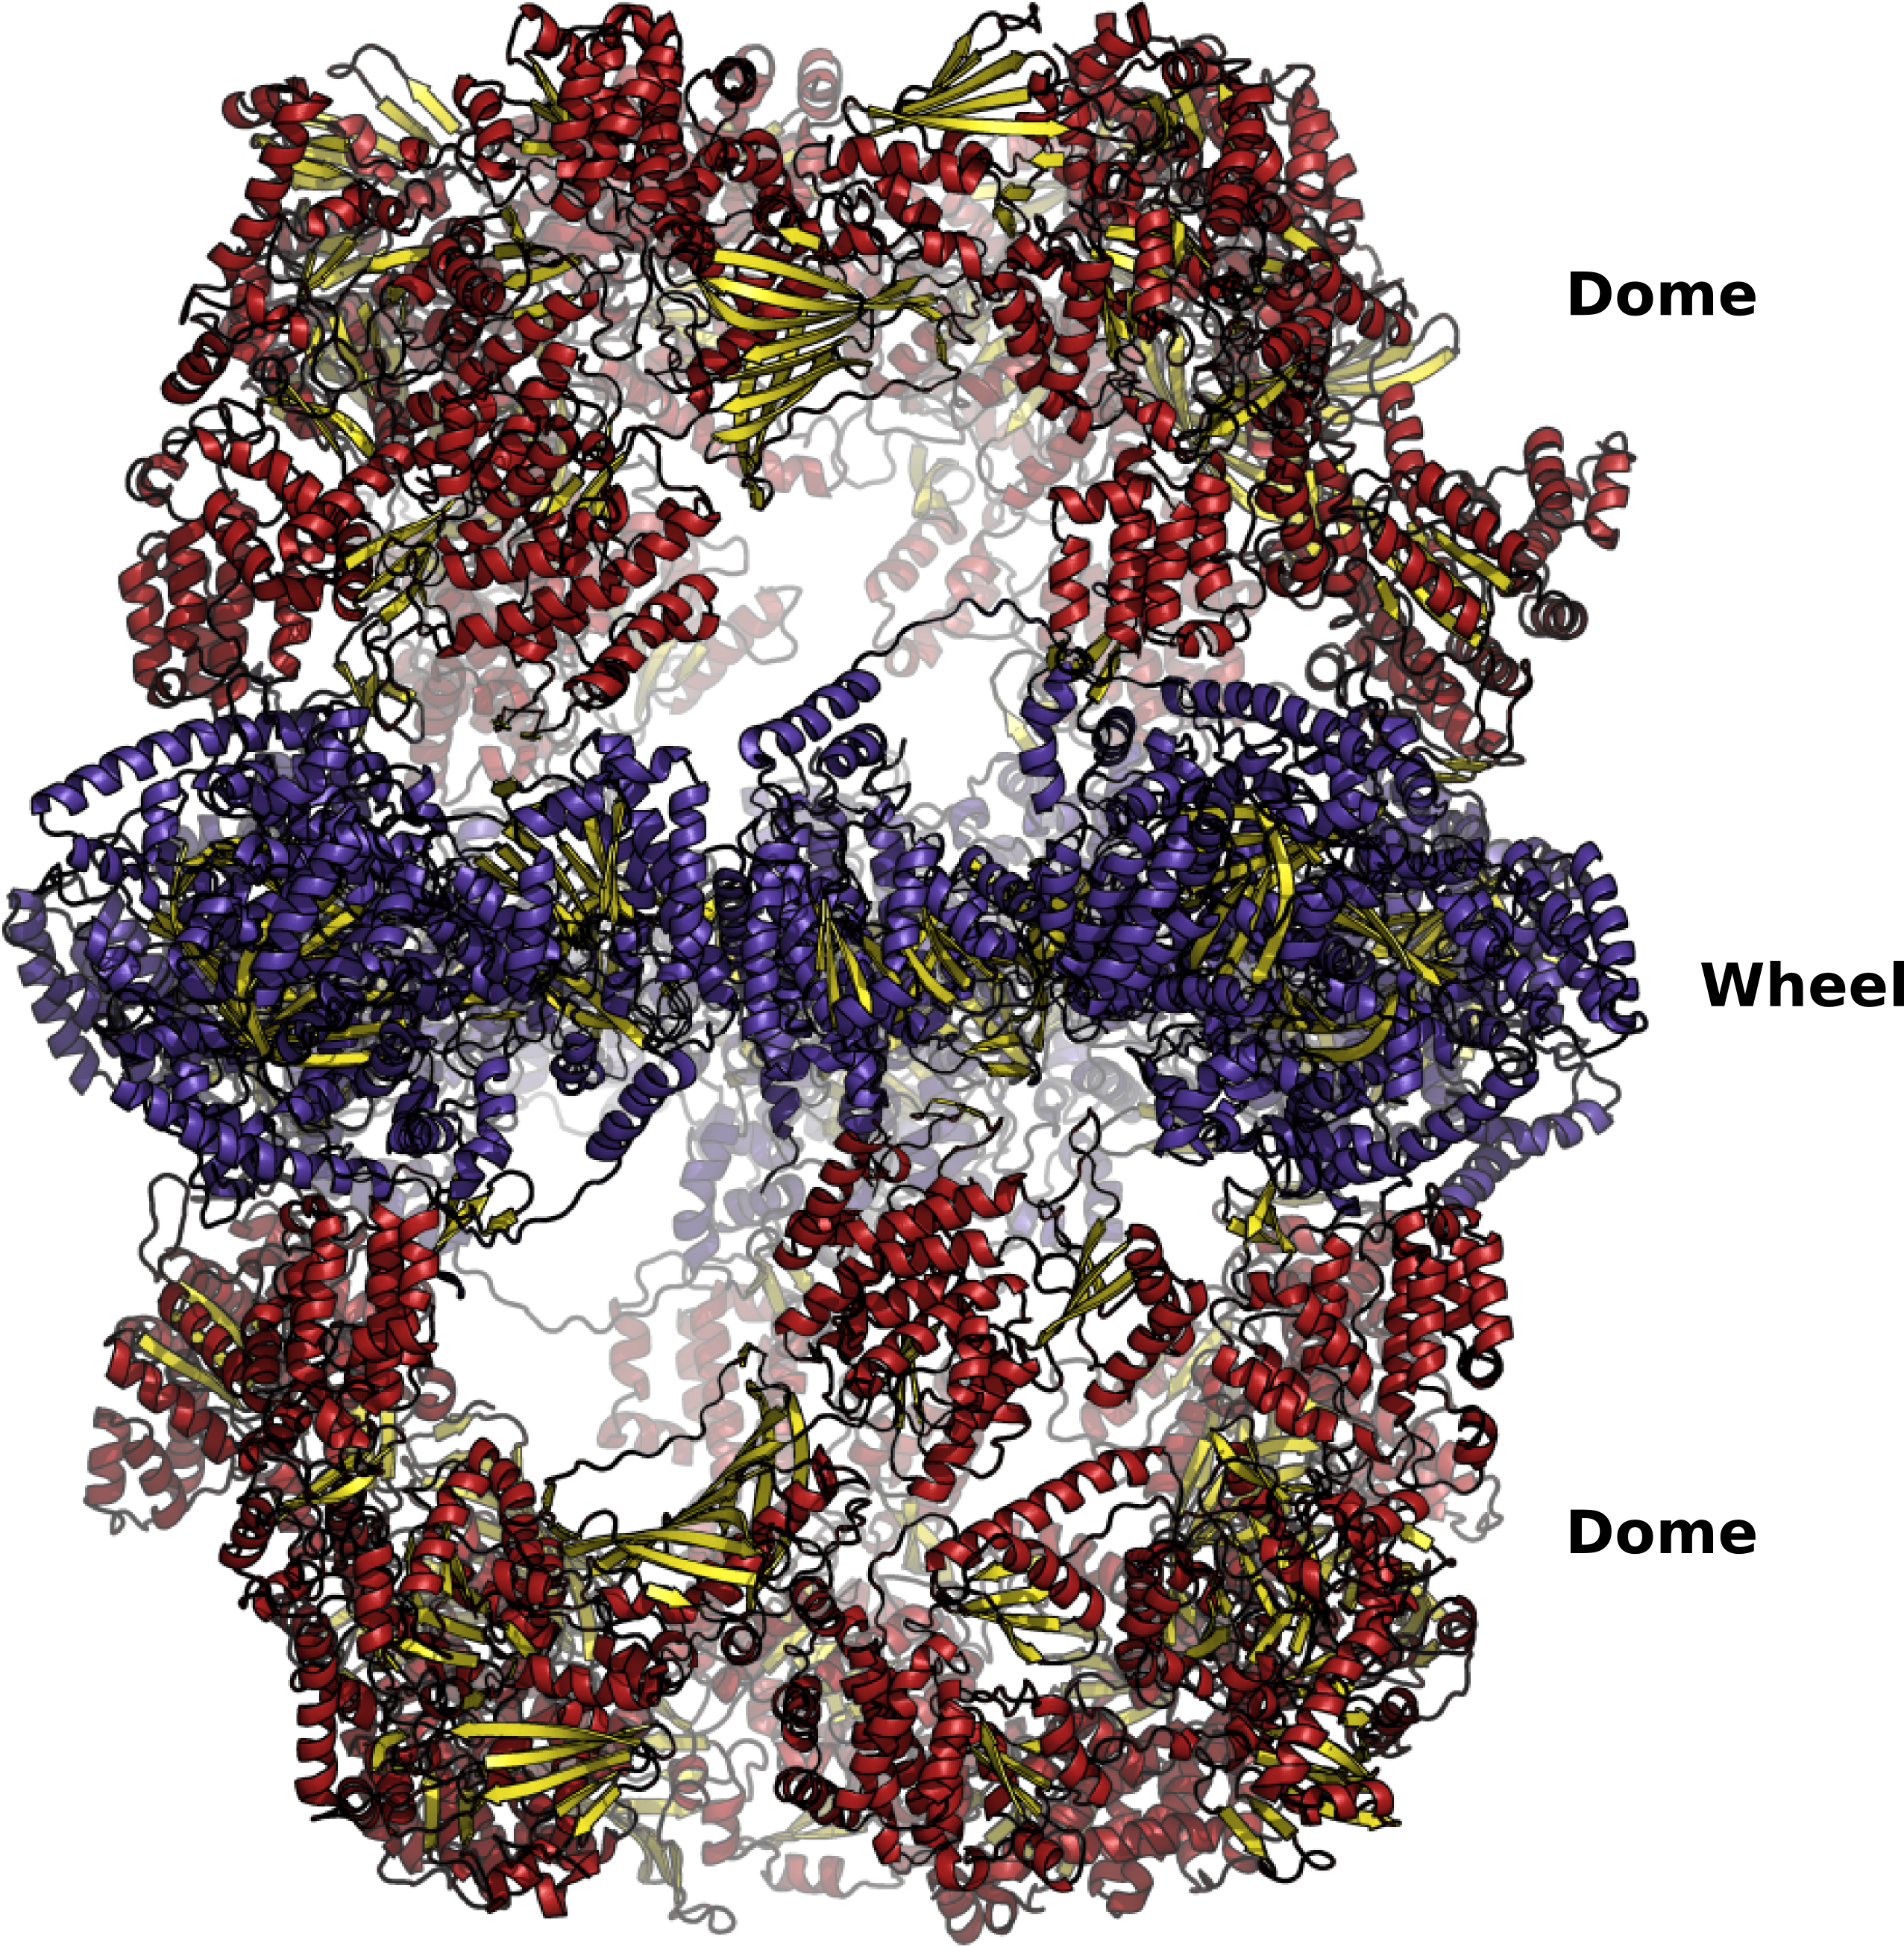
\includegraphics[width=0.95\textwidth, resolution=600, keepaspectratio=true]{graphics/mycoFasStructure.png}}
			\caption[X-ray structure of the mycobacterial FAS (PDB ID 4V8L) rendered as cartoon.]{X-ray structure of the mycobacterial FAS (PDB ID 4V8L) rendered as cartoon. Helices in the domes and the middle wheel are coloured in red and blue respectively. Beta sheets are coloured in yellow.}
			\label{fig:mycoFasStructure}
			\end{figure}			
					
		The \textit{Mycobacteium smegmatis} FAS is a 2.0 mDa $\alpha_{6}$ homohexameric structure coded as a single polypeptide containing all the catalytic domains as compared to the domains spread across two polypeptides in the fungal FAS. However, it lacked the phosphopantetheinyl transferase domain attached to the C-terminus. PPTs, called ACP synthases in \textit{Mycobacteria}, are standalone homotrimers encoded by a separate gene.This explains the presence of wider openings in the dome walls to let the ACP synthases reach the ACPs inside the reaction centres within the domes. %The AT domains in the \textit{Mycobacteria} have a conserved active site isoleucine which prevents any larger and charged substrates to be transferred on to an ACP. This suggest the role of MPT in recruiting larger substrate for the production of longer chain fatty acids.

\newpage		
		\subsubsection{\textit{Cis} and \textit{trans} AT PKS}
		\label{sec:ctPKS}
		Soon after the FAS structural elucidation by Ban's group the PKS community also released atomic resolution structural models for PKS systems. Khosla and colleagues were only able to crystallize the KS-AT homodimeric structures from DEBS 3$^{rd}$ and 5$^{th}$ modules \parencite{Tang2006, Tang2007}, and until very recently those were the only structures available for the PKS systems, which only represent part of the module. The first structure which came out was the 2.7 \AA{} resolution crystal structure of the 194 kD KS-AT homodimer from the module 5 of DEBS system (PDB ID 2HG4). This structure agreed very well with the then resolved 4.5 \AA{} resolution domain architecture structure of the mammalian FAS and was similar to the leg region of the mammalian FAS structure (Figure \ref{fig:debs2hg4tructure}). 

			\setlength\fboxsep{5pt}
 			\setlength\fboxrule{1.5pt}
			\begin{figure} []
			\centering
			\fbox{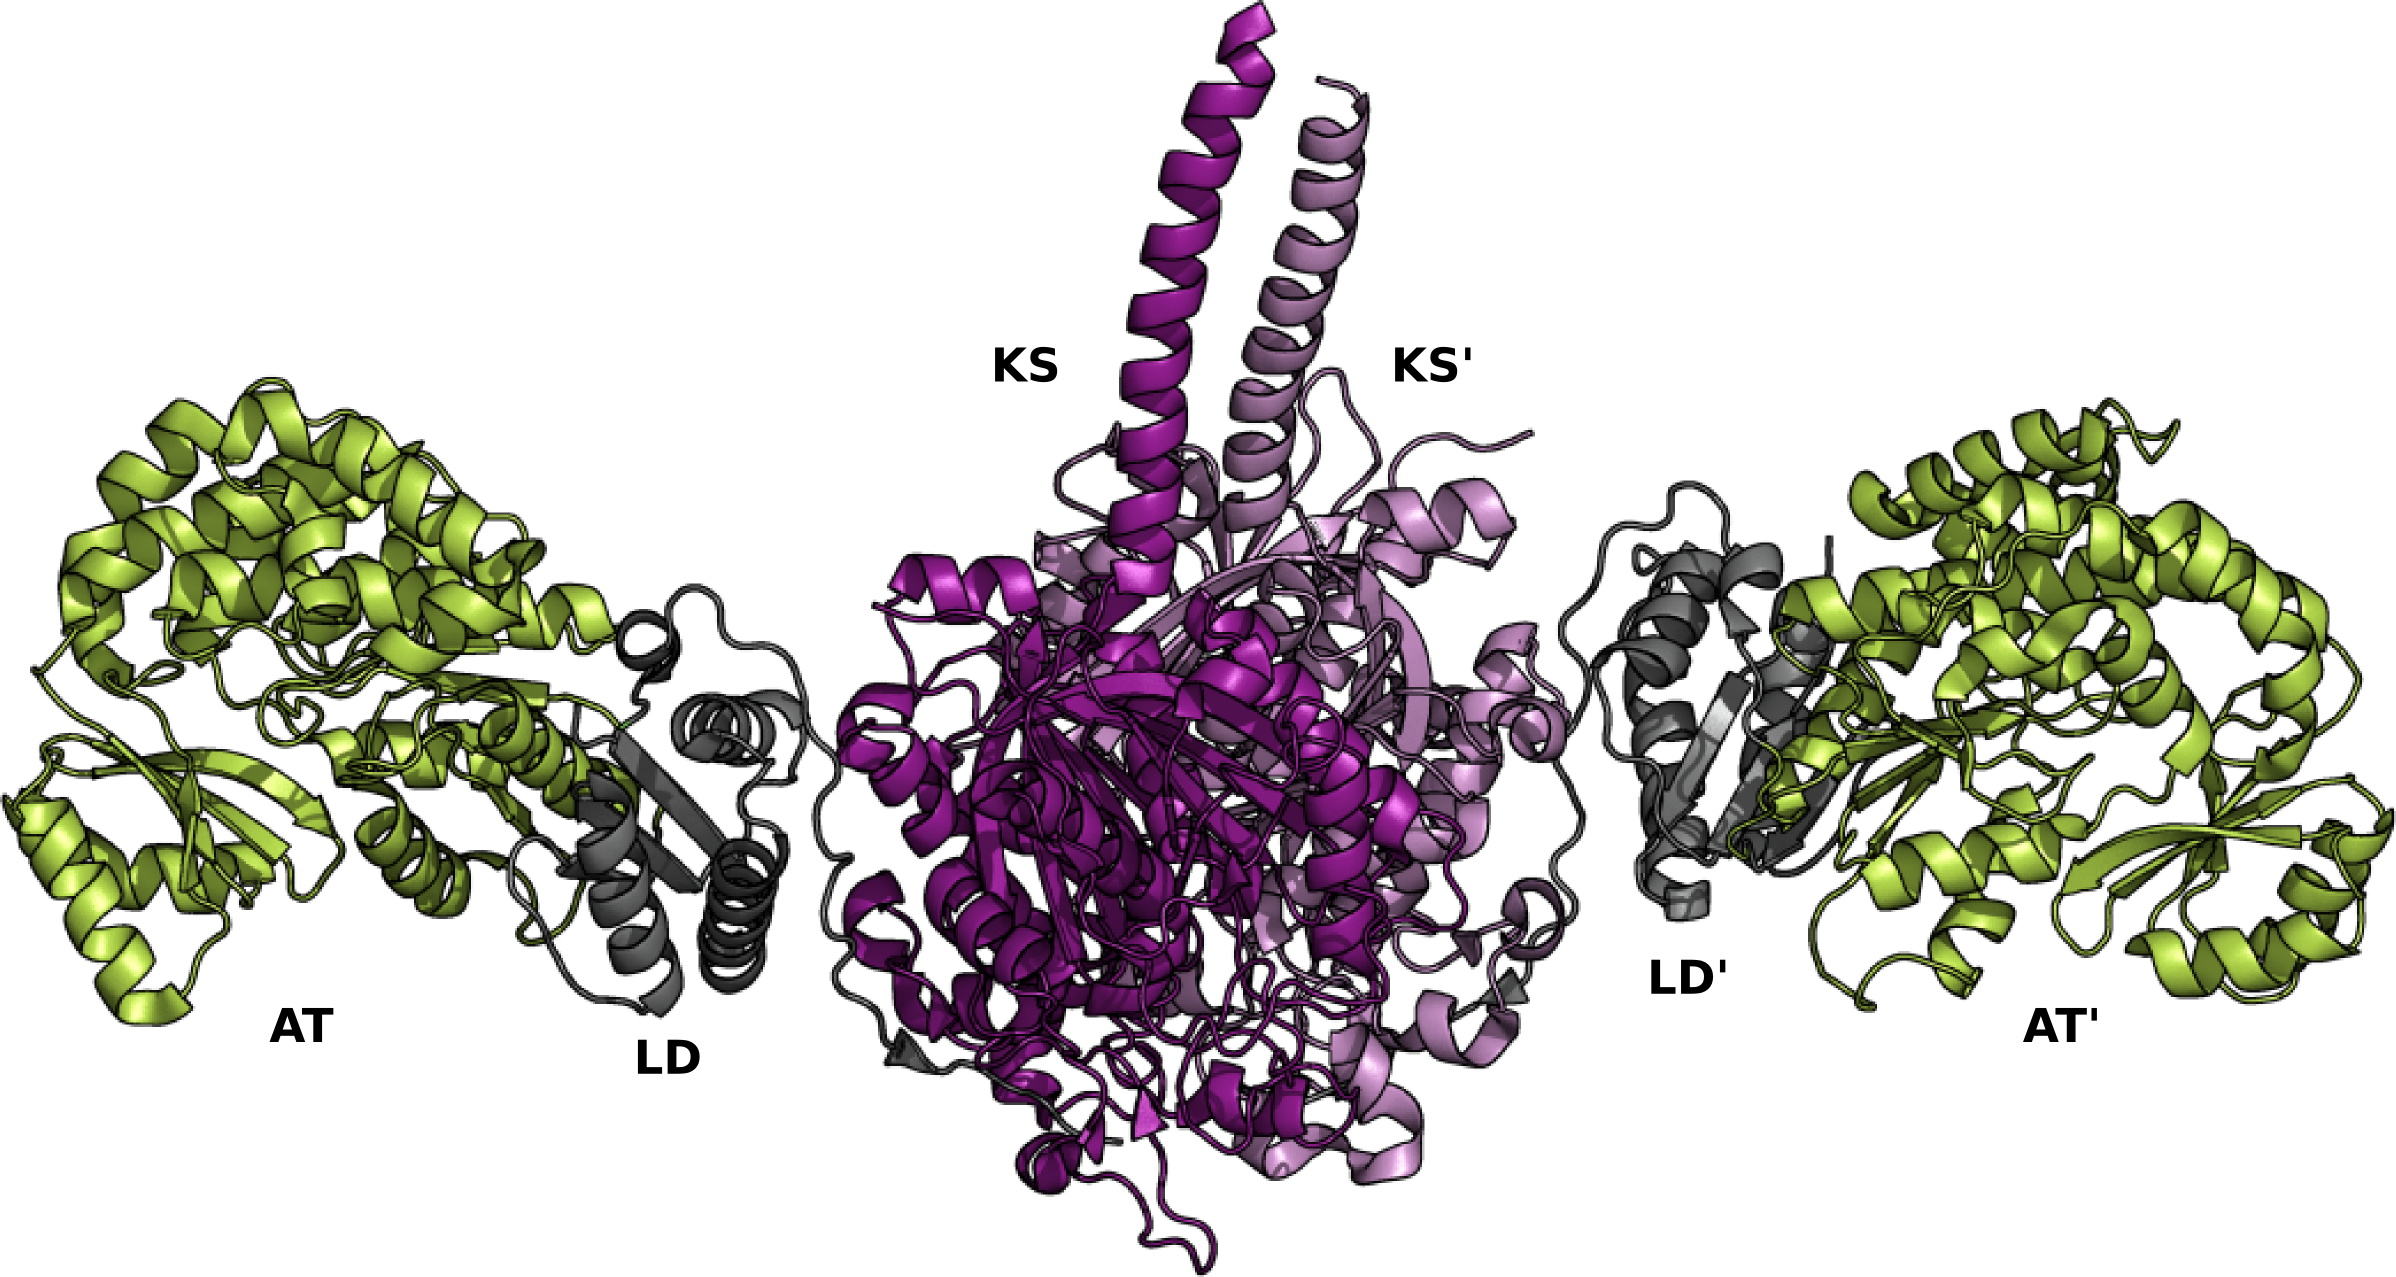
\includegraphics[width=0.95\textwidth, resolution=600, keepaspectratio=true]{graphics/debs2hg4Structure.png}}
			\caption[X-ray structure of the KS-AT homodimer from the DEBS (PDB ID 2HG4) system rendered as cartoon]{X-ray structure of the KS-AT homodimer from the DEBS (PDB ID 2HG4) system rendered as cartoon. Ketosynthase (KS) dimers are coloured in two different shades of purple, linker domains (LD) are coloured in grey and acyltransferase (AT) domains are coloured in lemon yellow.}
			\label{fig:debs2hg4tructure}
			\end{figure}					
		
		Apart from the two full length domain structures of the KS and AT domain the solved structure also had three linker regions. The N-terminal helical linker region, the linker region/domain between the KS and AT domains and the C-terminal linker which was thought to connect the AT and the KR domains. The KS domains form the dimer at the two fold axis and cover an area of 2,828 $ \AA{}^{2} $ at the interface. The KS domain fold was similar to their bacterial type II FAS counterpart and superimposed well with the \textit{E. coli} KS I domain. The N-terminal linker forms a helical dimer which protrudes outwards towards the solvent and does not make any contact with the rest of the protein complex. These linkers were thought to be involved in the inter modular interaction between the N-terminal linker of the KS domains with the C-terminal linker of the ACP from the previous module.  The two helices make hydrophobic contacts and a salt bridge between them. The well defined KS to AT linker region was formed by three $ \beta $-strands sandwiched between three $ \alpha $-helices from one side and two alpha helices from the other side contributed by the AT domains and the AT-KR linker forming an $ \alpha\beta\alpha $ fold. The C-terminus of the AT domain folds back towards the KS-AT linker and extends a further 30 aa extend across the surface of the KS, which presumably forms the linker between the AT and the KR, making 8 hydrogen bonds with the KS domain and 5 hydrogen bonds with KS-AT linker. Such a fold was not previously reported in the PDB. 
		
		Similar to the KS domains, AT domains also had the similar fold to that of the bacterial type II AT domains and superimposed well with the \textit{E. coli} AT domain, with the RMS deviation of 1.59 \AA{}. This structure also revealed an $\approx$80 \AA{} distance between the active site C199 and the S642 in the KS and AT domains respectively which suggested an extensive movement of the ACP domains in substrate channelling that would otherwise not be possible just by the phosphopantetheine arm of $\approx$20 \AA{}. 
		
		The active site of the KS domains also matched well with their bacterial type II homologues where it centres around the active site Cysteine reaching towards the dimer interface. The active site cleft was formed by the contribution of the residues from both the subunits and was connected via a tunnel to the outer opening at the surface of the KS domain. The residues lining the tunnel were highly conserved among the KS's homologue with the primary role of supporting the phosphopantetheine arm. Another interesting observation made through the KS-AT homodimer structure was the flexible loop region (residue 153-161) at the dimer interface which forms the part of the active site. This loop region is a helix in the type II KSs. It was hypothesized that this loop might be responsible for the KS specificity and helps in accommodating substrates of different size. This observation agreed well with the previous observations that the KS 5 can accommodate substrates of larger size than the native ligand \parencite{Tang2006}.
		
		The second structure solved by Khosla and colleagues was the 190kD KS-AT homodimer from the DEBS module 3 (PDB ID 2QO3, \textcite{Tang2007}). The overall fold of this strcutre was similar to the previously determined KS 5 structure however, it lacked the N-terminal linker region. The KS3 domain overlapped with the KS5 domain with an RMS deviation of 0.85 \AA{} for 386 backbone C$_{\alpha}$ atoms. One obvious difference was observed between the two KSs in the region from residue 71 to 91 (number according to KS3). This loop region on the surface in KS3 was longer as compared to the equivalent region in KS5. Sequence alignment with the other KSs from the DEBS system revealed that all the other KSs in the DEBS system were longer than KS5 by 12 residues in this region. 
		
		The KS-AT linker/domain in the KS3-AT3 structure also superimposed well with the KS5-AT5 linker region with an RMSD of 1.54 \AA{}. \textcite{Tang2007} also observed the difference in the active site lining residues in the KS3 and KS5 active sites. KS5 active site had fewer bulkier residues than KS3 active site, presumably to accommodate a larger substrate. They also found a conformational difference between a loop at the dimer interface from the residue 153 to 158 in the KS3 structure and residue 149 to 154 in the KS5 structure, the region that is a helix in type II KSs as explained above. Thus this loop region shows the importance not only in differentiating between the KS type I and type II but also exhibit differences between the same type from one KS to another. % on the basis of the nature of substrate. 		
		
		In 2014, for the first time, a complete modular structure for a PKS module was determined by \textcite{Dutta2014} for module 5 (PikAIII) in the pikromycin cluster from \textit{Streptomyces venezuelae}. The PikAIII consists of KS, AT, KR and ACP domains, the structure was determined by single particle electron microscopy (cryo-EM) at 7.5 to 9.5 \AA \ resolution. The cryo-EM maps were able to identify the secondary structures, which were used for the rigid body fitting of X-ray structures of the KS, AT, KR, and ACP domains from the DEBS system (Figure \ref{fig:emPksStructure}).

			\setlength\fboxsep{5pt}
 			\setlength\fboxrule{1.5pt}
			\begin{figure} []
			\centering
			\fbox{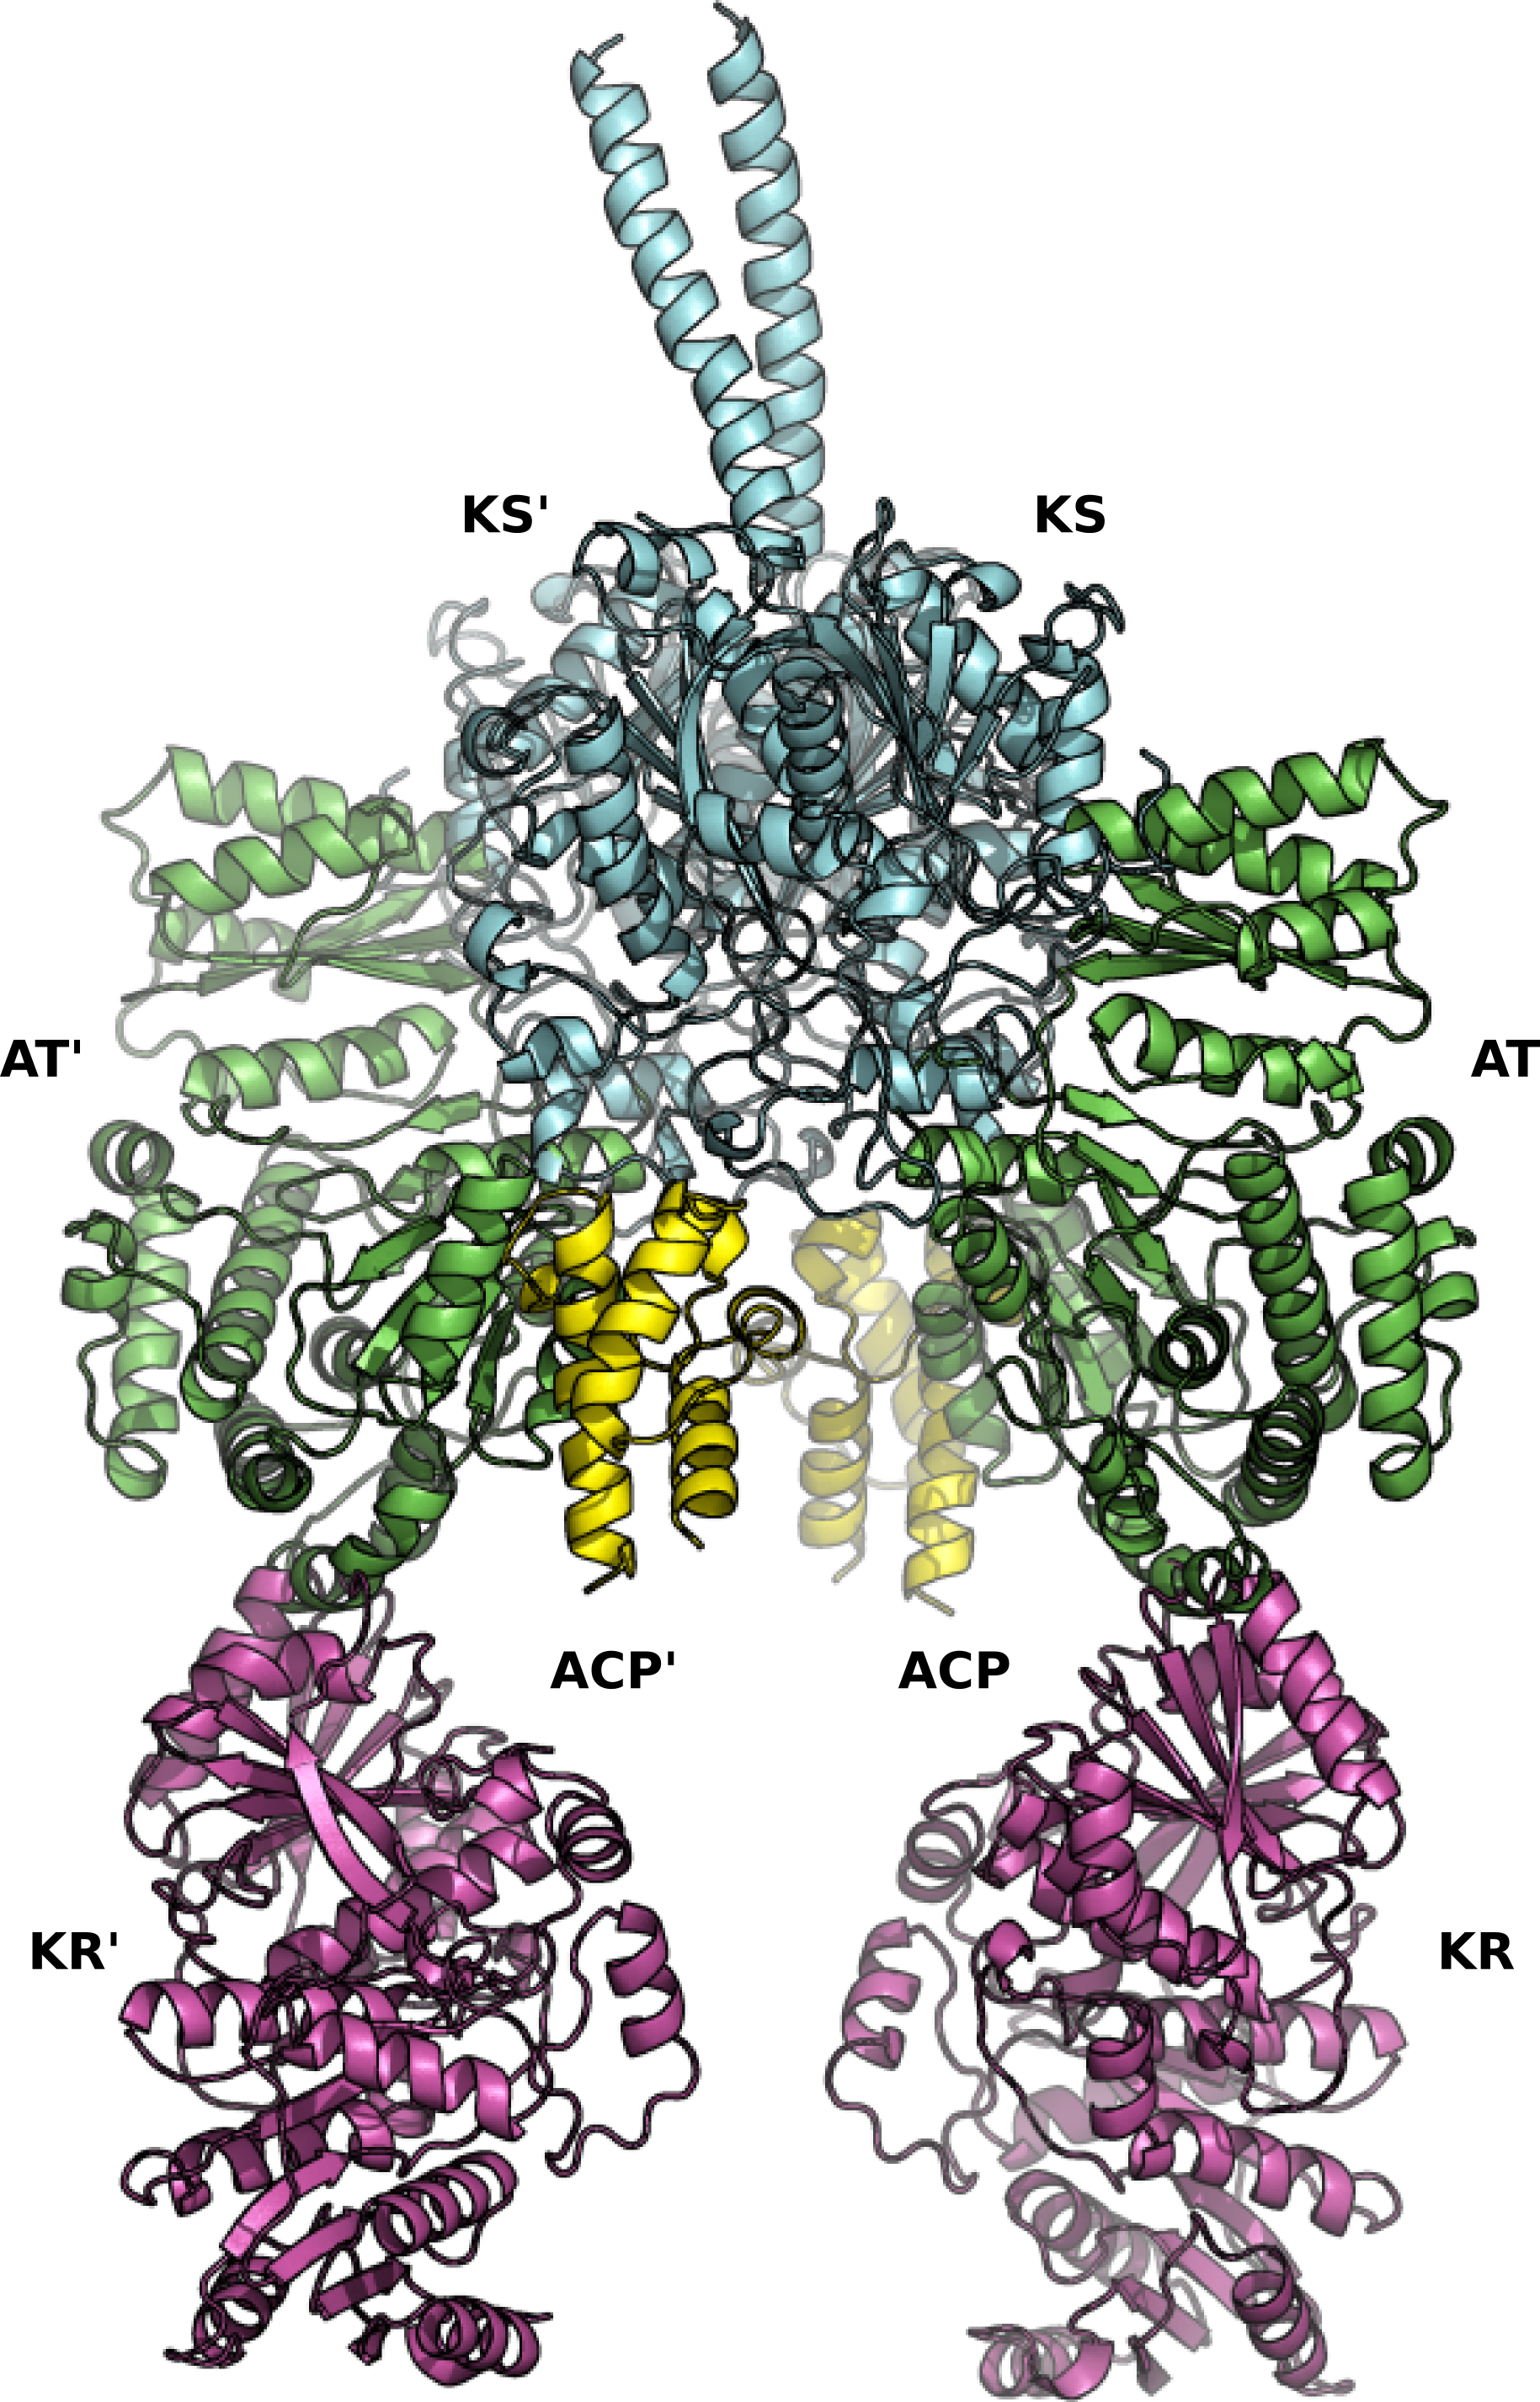
\includegraphics[width=0.80\textwidth, resolution=600, keepaspectratio=true]{graphics/emPksStructure.png}}
			\caption[EM structure of module 5 (PikAIII) from pikromycin cluster]{EM structure of module 5 (PikAIII) from pikromycin cluster. Ketosynthase (KS) dimers are coloured in cyan, acyl transferase (AT) domains are coloured in green, ketoreductase (KR) domains are coloured in magenta and acyl carrier protein (ACP) domains are coloured in yellow \parencite{Dutta2014}.}
			\label{fig:emPksStructure}
			\end{figure}					
					
		The EM structure revealed a striking difference between the PikAIII PKS module and the mammalian FAS structure which was till now considered to be the scaffold for the PKS modules as well. The PikAIII structure revealed a single reaction chamber utilized by that module's ACP to reach all the catalytic domains within the module, whereas the ACP from the previous module delivers the polyketide intermediated through a separate entrance outside the reaction chamber. The PikAIII symmetrical dimer folds into an arch shaped structure with KSs forming the dimer interface at the dome with the ATs hanging on either side of the KS dimer rotated at $ \approx $120\textdegree from their relative positions in mammalian FAS and also DEBS KS-AT dimer structures. The AT domains were also found to form an extensive interface with the KSs as compared to their counterparts in the mammalian FAS and DEBS KS-AT structures. The KR domains are lowered towards the base of the arch attached to the AT domains with the active sites of the AT and KR domains facing towards the reaction chamber. The ACPs were found either at the top, just below the KSs in between the two ATs, or at the base of the arch sandwiched between the two KRs. No evidence was detected for the two ACPs to be in different positions at the same time for example one near the ATs and the other near the KRs. 
		
		The cryo-EM maps also revealed that the linkers between the KRs and ACPs are long enough to reach both the KSs in the dimer. In another work from the same group, \textcite{Whicher2014} have shown a structural rearrangement of the KS-AT domains upon substrate binding in the PikAIII. In the parent paper,   \textcite{Dutta2014} have also shown that dimer formation of the PikAIII is not completely dependent on KS dimerization but is partly contributed by the post ACP dimerization helices. The presence or absence of the ACP domains was also found to  influence the orientation of the KR domains. In a PikAIII $ \Delta $ ACP5 strain, the KR domains were found to be rotated at $ \approx $165\textdegree about the axis of the arch legs. Upon expressing ACP4 from the previous module into the PikAIII $ \Delta $ ACP5 strain the ACP4 was found to be interacting at the N-terminal docking domain of the module 5 KSs, completely away from the reaction chamber where ACP5 would be found. This evidence established the involvement of a separate entrance for the acyl chain transfer on the KSs from an upstream module than utilizing the same reaction chamber involved in the chain elongation and \bet-carbon processing. In another unexpected observation KSs were found to have a second entrance to the active site for the entry of the extender units during elongation reaction. This second entrance was previously not reported either in the FAS or PKS structures. 
		
		\subsection{An example of re-engineering PKSs}
		\label{sec: reengineer}
		A number of groups have made contributions to our current understanding of PKS pathways and how to re-engineer them \parencite{Weissman2005, Challis2008, Piel2010, Kwon2012}, with the macrolide systems being particularly popular systems for study \parencite{Park2010}. Much work has been focused on the type I PKSs. For example, Khosla's group have extensively manipulated and modelled the DEBS system \parencite{Khosla2007}. In their work using a number of chimeric constructs of ACPs, crystal structure determination and computational protein-protein docking revealed how an ACP has specificity for the chain elongation in the DEBS pathway \parencite{Kapur2010}. How the same ACP specifically passes the processed substrate onto the next module \parencite{Kapur2010, Kapur2012}, and why a PKS dimer might be required for function.
		
		Chimeras of ACP3 and ACP6 from deoxyerythronolide B synthase, the ACPs from modules 3 and 6 of the synthetic pathway, indicate that the loop between helix I and helix II were critical during the elongation process of synthesis. Computer docking of the ACP onto the crystal structure of the KS5-AT5 homodimer indicated two residues in the loop that appeared critical for electrostatic complementarity (D44 and R45). Further modelling showed electrostatic complementarity between the KS-AT didomain in each module and the equivalent residues in their cognate ACP, ACP3 (R44, R45), ACP4 (R44, K45), ACP5 (D44, R45) and ACP6 (D44, Q45). Mutations R44A/R45A in ACP3 confirmed the importance of the residues at these positions. The authors noted that these key residues of the ACP interact with the linker (docking domain) between the KS and AT modules, as well as the AT module, and thus this mechanism cannot be the same for PKSs that have the AT acting in trans unless it docks in a similar orientation to the cis AT.
		
		In contrast to the elongation mechanism, for the transfer of the substrate from an ACP to the KS on the next module they found a different mechanism, one that relied on the $ 1^{st} $ ten residues in helix I of the ACP. They also concluded that the PKS domains are made up of subdomains and they have a distinct role in mediating interdomain interaction. These experiments also support the idea of homodimeric architecture of multimodular PKSs. This work emphasizes the benefit of computational modelling working together with well-designed experiments to elucidate the engineering principles underlying the PKS.
		
		From understanding the principle behind the ACP-KS recognition in the polyketide chain elongation and translocation steps, an obvious question arises. Is there a way that this unidirectional ratchet flow of the pathway can be modified? Khosla's group identified a charge complementarity mechanism during chain elongation at the position 23 on the ACP at the KS-AT interaction interface. They found that the opposite charge on KS-AT linker of the following module attracts the preceding ACP, whereas the similar charge on the KS-AT linker of the parent module repels it, thus allowing the reaction to always move forward. Exploiting this mechanism they re-programmed module 3 of the DEBs system to carry out an iterative step of chain elongation. In an experiment they swapped the helix I of ACP3 with the helix I of ACP2, as the helix I is responsible for the chain elongation step. This swapping did not allow the ACP3 to transfer the chain to the module 4 instead it falls back to the KS3 in the module 3 for one more round of chain elongation. The reaction stopped after one round of iterative chain elongation for reasons unknown. However, it could be a limitation of the KS active site to accommodate the larger substrate.
		
	\section{NRPS}
	\label{sec:NRPS}
	Nonribosomal peptide syntetases (NRPSs) are also highly prevalent in secondary metabolite biosynthesis and often synthesize compounds in conjunction with PKSs. The NRPS and PKS systems have similar modular structures and thus NRPSs warrant some discussion here. Nonribosomal peptides are the product of the sequential addition of amino acid monomers catalyzed by NRPSs, involving the domains similar in function to that of PKS system. The amino acid monomers are selected and activated by an adenylation (A) domain which transfers to a thiolation domain or a peptide carrier protein (T or PCP), peptide bond formation is catalyzed by a condensation (C) domain. The PCP has a phosphopantetheine prosthetic group that facilitates the transfer of growing peptide chain/monomers to the various active sites and function analogously to an ACP with a similar four helix bundle structure. The adenylation (A) domain, condensation (C) domain and thiolation or peptide carrier protein (PCP) form the minimal set of domains required to carry out the NRP biosynthesis. In both, the modular PKS and NRPS system the individual domains are linked together by a polypeptide linker region which has also been found to be responsible for functional communication within the domains.
	
	\section{Mupirocin}
	\label{sec:Mup}
	Mupirocin is a polyketide antibiotic used as a topical drug against MRSA and various other  Gram positive bacteria, to treat bacterial skin and hospital acquired infections \parencite{Fuller1971}. Mupirocin is produced by \textit{Pseudomonas fluorescens} NCIMB 10586 and consists of four different pseudomonic acids (PAs) A,B,C and D. PA A, B, C, D contributes 90\%, 8\%, \textless2\% and \textless2\% respectively to the mixture. PAs are made up of monic acid esterified to 9-hydroxynonanoic acid (Figure \ref{fig:mupirocin}). Mupirocin acts by inhibiting bacterial isoleucine tRNA synthetase \nomenclature{IleRS}{Isoleucine tRNA synthetase} thus inhibiting protein production resulting in the cell death \parencite{Hughes1978}.
	
	\setlength\fboxsep{5pt}
	\setlength\fboxrule{1.5pt}
	\begin{figure} []
	\centering
	\fbox{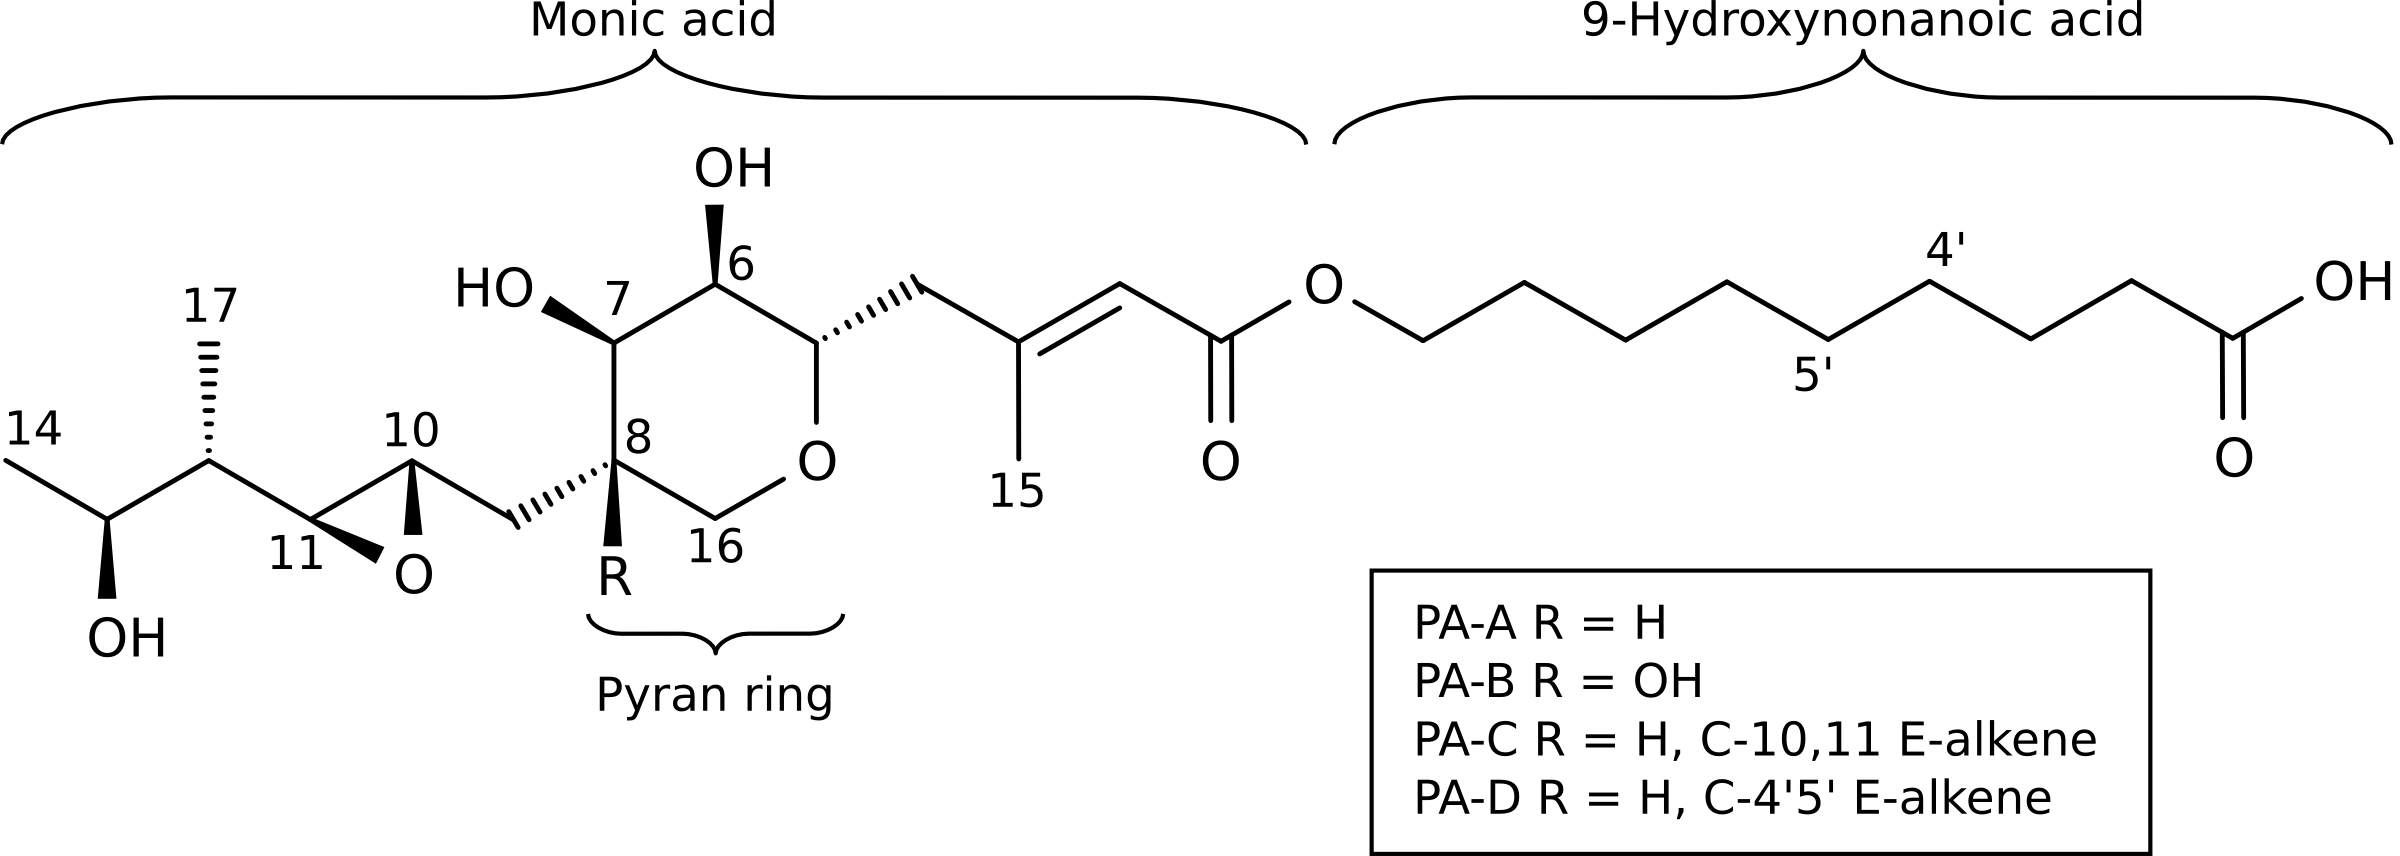
\includegraphics[width=0.8\textwidth, resolution=600, keepaspectratio=true]{graphics/mupirocin.png}}
	\caption[Mupirocin structure]{Mupirocin structure}
	\label{fig:mupirocin}
	\end{figure}
	
		\subsection{Mupirocin Drawbacks}
		\label{sec:MupDrawbacks}
		Mupirocin has proved to be more potent on bacterial IleRS than on the corresponding eukaryotic enzyme, which is highly desirable for any pharmaceutical product. Weak affinity for the eukaryotic IleRS minimises the chances of eukaryotic toxicity and side effects of the drug. Thus, the pseudomonic acids have excellent structures and biological activity as pharmaceutical compounds. However, mupirocin can only be used as a tropical drug as it gets disintegrated inside the body by the hydrolysis of the ester bond between monic and 9-hydoxynonanoic acid (Figure \ref{fig:mupirocin}). It also loses its activity at higher pH, thus preventing it from being used as a systemic drug.
		
		Recent studies \parencite{Patel2009, Thomas2010} have also shown increasing occurrences of mupirocin resistance in \textit{S. aureus}. This resistance can be of low level as well as high level. In low level Mupirocin resistance a single amino acid mutation has been observed in the Rossmann fold region of IleRS, which normally binds to the ATP or else to the 9-hydroxynonanoic acid of Mupirocin. Hence the single amino acid change prevents Mupirocin from inhibiting its target. High level resistance usually results from the presence of eukaryotic like IleRS. This can be acquired either through horizontal gene transfer or through a plasmid containing the mupA gene. The \textit{P. fluorescens} strain, which produces mupirocin, has two different IleRS producing genes of which one is similar to eukaryotic IleRS. This eukaryotic similar IleRS enables \textit{P. fluorescens} to keep on synthesising proteins even at high concentration of Mupirocin. Low-level resistance is not of present concern but the high-level resistance in clinical strains of \textit{S. aureus} acquired through the expression of the mupA gene is alarming. Many of the plasmids containing these genes can conjugate which may cause clonal expansion of the resistant strains.
		
		Therefore with increasing levels of Mupirocin resistance and its limitation for systemic use, there is a need to develop new analogues which may overcome the limitations of Mupirocin. However, before we reach up to the level of producing new analogues we need to understand better the underlying pathway.
		
		\subsection{Mupirocin Biosynthesis}
		\label{sec:MupBiosynthesis}
		The mupirocin biosynthetic cluster (\textit{mup}) consists of a 75kb region encoding 35 ORFs. Figure 1.5 explains the mup cluster and the probable pathway as proposed by Thomas and co- workers \parencite{Thomas2010, Gurney2011}. The \textit{mup} cluster encodes six designated MMPs (Mupirocin multifunctional proteins; \textit{mmpA} to \textit{mmpF}) out of which five encode for polyketide synthases. The non-PKS domain is MmpC, encoding two acyltransferase domains, which is a characteristic of a trans AT system. The proposed biosynthesic pathway initiates in a typical Type I PKS manner where MmpD holds the first starter unit and produces a C$ _{12} $ unit, with MmpA extending this to  C$_{17} $, with further tailoring enzymes producing monic acid. MmpD and MmpA consist of four and three modules respectively each containing a KS and ACP domain. MmpD also consists of KR, DH and MT domains while MmpA only has one KR domain. The first module in MmpD has a non-functional DH and the first module in MmpA is proposed to be involved with the transfer of the growing polyketide chain from MmpD to MmpA. Mupirocin biosynthesis starts with an activated acetyl as a starter unit and uses malonyl-CoA as an extender unit. C$_{16} $ and  C$_{17} $ carbons in the monic acid unit are derived from S-adenosyl methionine (SAM).

		\setlength\fboxsep{5pt}
		\setlength\fboxrule{1.5pt}
		\begin{sidewaysfigure} []
		\centering
		\fbox{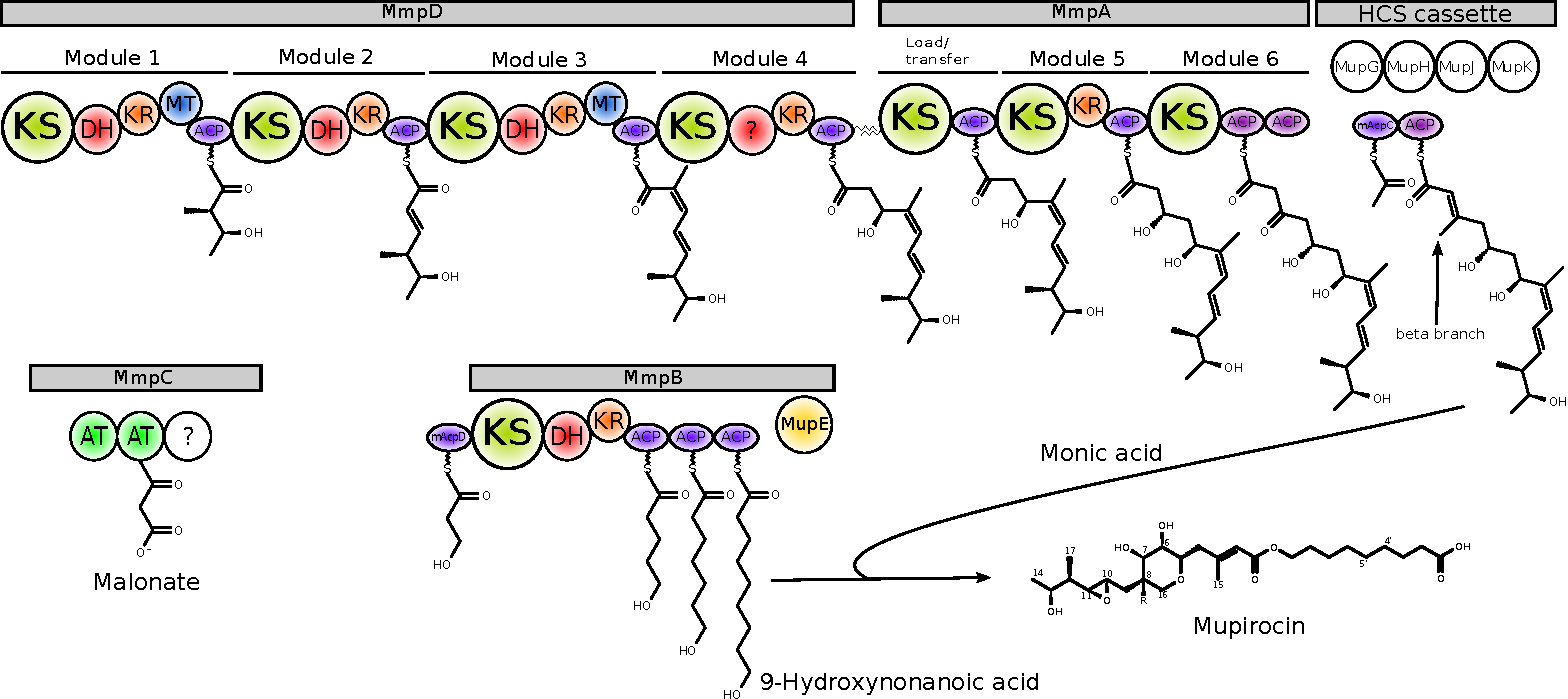
\includegraphics[width=\textwidth, resolution=600, keepaspectratio=true]{graphics/muppathway.pdf}}
		\caption[Mupirocin biosynthesis pathway]{Mupirocin biosynthesis pathway. Figure adapted from \parencite{Thomas2010}.}
		\label{fig:muppathway}
		\end{sidewaysfigure}
					
		The C$_{15} $ carbon is hypothesised to be incorporated by the HMG-CoA synthases activity of MupH in the HCS cassette (MupG, MupH, MupJ and MupK). Knocking out any of the HCS genes stalls the pathway at the end of MmpA and results in the accumulation of intermediate mupirocin H. \parencite{Wu2007}. The HCS cassette has at least four enzymatic functions: an ACP, a hydroxymethyl glutaryl-CoA synthase, a decarboxylase and one or more dehydratases from the crotonase superfamily, in some cases supplemented with other functions. HCS cassettes variously introduce e.g. \bet-methyl, cyclopropane and vinyl chloride moieties, depending on the system they are found in and the exact nature of the cassette. HCS cassettes are found to act on the type I modules, which lack KR, DH or ER domains but which  tend to have tandemly repeated ACPs. Given the variety of functions that the HCS cassette can perform, artificially including them in a PKS cluster provides a powerful tool for the synthesis of novel compounds. To achieve this we need to understand what allows the enzymes of the cassette to know at what point in the pathway they are supposed to work, in particular how a system such as myxovirescin uses two HCS cassettes to produce two specific $ \beta $ modifications in the same system.
		
		\textit{MupC, mupF, mupO, mupU, mupV} and \textit{macp}E provides the correct oxidation state around the pyran ring and mutating any of these genes would result in the accumulation of pseudomonic acid B. Whereas MupT and MupW are hypothesised to be involved in the activation of methyl group C$_{8} $  in order to create the pyran ring.
		
		Finally, MmpB is proposed to synthesise 9-hydroxynonanoic acid starting from 3-hydroxy-propionate via three condensations with malonate iterated three times in the same PKS.  3-hydroxypropionate starter unit is hypothesized to be produced jointly by mAcpD, MupS and MupQ. It is also not understood whether 3-hydroxy-propionate is first attached to mAcpD and then elongated to produce 9-hydroxynonanoic acid or is first esterified to monic acid and then elongated further.
		
		The mupirocin biosynthesis pathway has an ACP doublet (ACPmupA3a/b in MmpA) and an ACP triplet (ACP5, 6 and 7 in MmpB) which is thought to hold multiple substrates for high throughput in rate limiting steps. Apart from the six orfs, which code for the Mmps, the rest of the orfs encode for discrete polypeptides.
		
	\section{Bioinformatics approaches in PKS research}
	\label{sec:BioinfoPKS}
	Research into PKS pathways has been carried out in two major areas. Firstly to identify and experimentally characterize new polyketide natural products and secondly, to develop a synthetic biology tool box for the design and synthesis of novel “natural” products by the re-engineering of naturally occurring polyketide biosynthetic machinery, both of which might provide the basis for novel drugs. Bioinformatics analysis of PKS clusters has played a major role in guiding recent experiments via a variety of tools, examples are PKSDB \parencite{Yadav2003} a database of PKS domains developed a decade ago, which was one of the first tools available, SBSPKS \parencite{Anand2010} and antiSMASH \parencite{Medema2011}, which are recent advanced sequence analysis tools guided by protein structure analysis.
	
	Most work in the field has focused on the core PKS functions, particularly type I PKSs, thus there is still little known about the mechanisms of the tailoring enzymes acting in trans. Such tailoring enzymes are an essential part of any PKS system since they provide additional chemical diversity to the polyketide chain. An ability to predict the function of tailoring enzymes and their compatibility with other PKS modules would provide much additional functionality to the synthetic biology tool box. \textit{Trans}-AT systems are less well studied and since software tools are primarily targeted at \textit{cis}-AT systems they tend to completely fail or have limited capabilities in predicting \textit{trans}-AT systems.
%	
	PKSDB/SEARCHPKS and NRPS-PKS were the first available webservers for identifying PKS/NRPS domains in an unknown sequence as well as relating PKS/NRPS sequences to their corresponding secondary metabolites; recent reviews \parencite{Jenke-Kodama2009, Bachmann2009} give a detailed discussion on the utility of the PKSDB and the NRPS-PKS databases. Following similar lines, resources like ASMPKS \parencite{Tae2007}, ClustScan \parencite{Starcevic2008}, CLUSEAN \parencite{Weber2009}, NP.searcher \parencite{Li2009}, NRPSpredictor \parencite{Rottig2011}, NRPSsp \parencite{Prieto2012} and antiSMASH \parencite{Medema2011} have been developed for the discovery of secondary metabolites through genome analysis. All these servers primarily utilize sequence information either for domain identification or to correlate the various PKS domains to their corresponding metabolic products. However, many of them also utilize structural information for predicting the most likely starter and extender units picked by the acyl transferase domains, and SBSPKS models the 3D structure of PKS modules. Table  \ref{tab:pks_res} gives a summary of the resources available for PKS/NRPS pathway analysis with a detailed description in Section \ref{sec:comptools} of Appendix IV.
%		
\newpage		
		\begin{singlespace}
		\begin{small}
		\begin{longtabu}[tbp]{p{2.5cm} p{2cm} p{2cm} p{2cm} p{2cm} p{2.5cm}}
		\caption{Resources available for secondary metabolite prediction.}
		\\ \hline\hline\hline
		 \bf{Resources} & \bf{Clusters/ types} & \bf{Prediction tools} & \bf{Domain for which specifity is predicted} & \bf{Backend or Training data source} & \bf{Hyperlink} \\ \hline\hline\hline
		SEARCHPKS, PKSDB (database) & PKS & BLAST & AT & PKSDB & \url{http://www.nii.res.in/searchpks.html} \\ \hline
		NRPS-PKS (database) & NRPS, PKS & BLAST & AT, A	& PKSDB, NRPSDB, ITERDB, CHSDB & \url{http://www.nii.res.in/nrps-pks.html} \\ \hline
		ASMPKS & PKS & GLIMMER, BLAST & AT & PKSDB, More & \url{http://gate.smallsoft.co.kr:8008/~hstae/asmpks/genome.pl} \\ \hline 
		NRPSpredictor, NRPSpredictor2 & NRPS & SVM, TSVM & A & Training data amalgamated from various sources &	\url{http://nrps.informatik.uni-tuebingen.de/Controller?cmd=SubmitJob} \\ \hline 
		CLUSTSCAN, CompGen (homologous recombination module) & PKS, NRPS, PKS-NRPS hybrid & HMM	& KR, AT & Pfam, Specialized & \url{http://bioserv.pbf.hr/cms/}, \url{http://bioserv.pbf.hr/cms/index.php?page=compgen} \\ \hline
		SBSPKS & NRPS, PKS & BLAST, 3D structure modelling & AT, A & PKSDB, NRPSDB, ITERDB, CHSDB & \url{http://www.nii.ac.in/~pksdb/sbspks/master.html} \\ \hline
		NORINE (database) & NRPS products, monomers & & & & \url{http://bioinfo.lifl.fr/norine/} \\ \hline
		CLUSEAN (Perl module framework)	& NRPS, PKS & BLAST, HMM & A & NCBI NR, Pfam, Specialized & \url{http://redmine.secondarymetabolites.org/projects/clusean} \\ \hline
		antiSMASH (metaserver \& standalone) & NRPS, PKS, terpenes, aminoglycosides, amino-coumarins, indolocarbazoles, lantibiotics, bacteriocins, nucleosides, β-lactams, butyrolactones, siderophores, melanins and others & NCBI BLAST+, HMMer, Muscle, Glimmer, FastTree, TreeGraph & AT, A, KR & Amalgamated from various previously published works	& \url{http://antismash.secondarymetabolites.org/} \\ \hline\hline\hline
		\label{tab:pks_res}
		\end{longtabu}
		\end{small}
		\end{singlespace}

	\section{Research objectives and thesis outline}
	\label{sec:researchobjectives}
	The mupirocin biosynthesis pathway provides a model system for understanding \textit{trans}-AT PKSs, and contributing to our understanding of the way proteins and substrate recognition events are regulated. In the present work the analysis was mainly focused on the structural modelling of the protein complexes involved in the mupirocin synthesis via the tools of structural bioinformatics supplemented with information from experiments. The findings in this thesis will be a prototype for the modelling of large macromolecular complexes in prokaryotic systems and the structural models produced will enhance our understanding of the synthetic pathways allowing us to re-engineer them with greater success. 
	
	The overall thesis is divided into four results chapters Chapter 3 to 6, which discuss the results of three major projects in their respective chapters and two minor projects compiled in one chapter. Chapter 2 describes the methods used in the different projects in detail. The last chapter of the thesis summarizes and discusses the entire thesis. 
	
	The project discussed in Chapter 3, aimed to elucidate the mode of interaction between ACP-mupA3ab:MupH complex, which are involved in beta branching, proposing key interacting residues for mutagenesis experiments. Structural models and properties of MupH the HMG-CoA synthase homologue in HCS cassette were predicted using various bioinformatics tools. ACP sequences from characterised PKS pathways were also classified into beta and non-beta branching type using hidden Markov model analysis. Mutagenesis experiments carried out by Prof. Thomas' group on the predicted ACP:MupH interface supports the predicted complex and residues responsible for the specificity of the interaction. Some of the findings of this project are already published in \textcite{Haines2013}.
	
	Based on the hypothesis generated in the first project, further lab experiments were carried out as described in Chapter 4. The aim was to complement the \bet-branching-ACPs in the mupirocin cluster with the \bet-branching-ACP(s) from the kalimantacin cluster. It was hypothesized that the \bet-branching ACP(s) from the kalimantacin cluster would not work with MupH but will work with BatC (MupH equivalent form kalimantacin cluster). The aim was also to identify the key residues at the interface of the \bet-branching ACPs from the \textit{mup} cluster and BatC which can be modified to work efficiently with BatC.
	
	As the experiments and molecular dynamics (MD) simulations carried out on FAS ACPs \parencite{Chan2008} have shown the formation of a hydrophobic tunnel which sequesters the fatty acid chain, the third project was to see if a similar mechanism might exist in the PKS ACPs. Molecular dynamics simulations of the ACPs from module 2 and 3 of MmpA in the mupirocin cluster were carried out in explicit solvent with a time scale of 50 ns to 1 $ \mu $s. Several macroscopic properties were calculated by analysing the MD simulation trajectories, a sequestering of the substrate to the ACP surface was seen but the atomic details are different from what was seen in the FAS system. 
	
	Chapter 6 presents the results of two independent projects, the first project aimed to find out the means of recognition specificity of the KS-mupA2 towards the predicted $ \alpha $-OH substituted substrate and the results suggest a specific recognition motif that may stall substrate progression until it has been hydroxylated. The second project aimed to investigate the significance of movements of loops on the MupH surface that were seen in the simulations presented in Chapter 4. Simulations suggested the loops may leave easy access to the active site until the substrate is bound.
	

	

\nomenclature{Mup}{Mupirocin cluster}
\nomenclature{Mmp}{Mupirocin multi functional proteins}
\nomenclature{MD}{Molecular dynamics}
\nomenclature{6-MSA}{6-methyl-salicylic acid}
\nomenclature{HCS}{3-hydroxy-3-methyl glutryl-CoA synthase cassette}
\nomenclature{HMG-CoA}{3-hydroxy-3-methyl glutryl-CoA}
\nomenclature{MS}{Mass spectrometry}
\nomenclature{bp}{Basepair}
\nomenclature{DEBS}{6-deoxyerythronolide B synthase}
\nomenclature{MAT}{Malonyl transferase}
\nomenclature{MT}{Methyl transferase}
\nomenclature{SNAC}{Sodium 8-((2-hydroxybenzoyl)amino)octanoate}
\nomenclature{SDR}{Short chain dehydrogenases/reductases}
\nomenclature{NADPH}{Nicotinamide adenine dinucleotide phosphate}
\nomenclature{MDR}{Medium chain dehydrogenase reductases}
\nomenclature{PPT}{Phosphopantetheinyl transferase}
\nomenclature{MRSA}{Methicillin-resistant \textit{S. aureus}}
\nomenclature{INSDC}{International Nucleotide Sequence Database Collaboration}
\nomenclature{CDS}{coding sequences}
\nomenclature{PSI-BLAST}{Position Specific Iterative - Basic Local Alignment Search Tool}
\nomenclature{PSSM}{Position specific scoring matrix}
\nomenclature{PHI-BLAST}{Pattern Hit Initiated - Basic Local Alignment Search Tool}
\nomenclature{HMM}{Hidden Markov model}
\nomenclature{SASA}{solvent accessible surface area}
\nomenclature{EDTA}{Ethylenediaminetetraacetic acid}
\nomenclature{TAE}{Tris Acetate EDTA}
\nomenclature{TTC}{Triphenyl tetrazolium chloride}
\nomenclature{AIR}{Ambiguous interaction restraints}
\nomenclature{MSA}{Multiple sequence alignment}